%%%%%%%%%%%%%%%%%%%%%%%%%%%%%%%%%%%%%%%%%%%%%%%%%%%%%%%%%%%%%%%
%% OXFORD THESIS TEMPLATE

% Use this template to produce a standard thesis that meets the Oxford University requirements for DPhil submission
%
% Originally by Keith A. Gillow (gillow@maths.ox.ac.uk), 1997
% Modified by Sam Evans (sam@samuelevansresearch.org), 2007
% Modified by John McManigle (john@oxfordechoes.com), 2015
% Modified by Ulrik Lyngs (ulrik.lyngs@cs.ox.ac.uk), 2018, for use with R Markdown
%
% Ulrik Lyngs, 25 Nov 2018: Following John McManigle, broad permissions are granted to use, modify, and distribute this software
% as specified in the MIT License included in this distribution's LICENSE file.
%
% John tried to comment this file extensively, so read through it to see how to use the various options.  Remember
% that in LaTeX, any line starting with a % is NOT executed.  Several places below, you have a choice of which line to use
% out of multiple options (eg draft vs final, for PDF vs for binding, etc.)  When you pick one, add a % to the beginning of
% the lines you don't want.


%%%%% CHOOSE PAGE LAYOUT
% The most common choices should be below.  You can also do other things, like replacing "a4paper" with "letterpaper", etc.

% This one will format for two-sided binding (ie left and right pages have mirror margins; blank pages inserted where needed):
%\documentclass[a4paper,twoside]{templates/ociamthesis}
% This one will format for one-sided binding (ie left margin > right margin; no extra blank pages):
%\documentclass[a4paper]{ociamthesis}
% This one will format for PDF output (ie equal margins, no extra blank pages):
%\documentclass[a4paper,nobind]{templates/ociamthesis}
%UL 2 Dec 2018: pass this in from YAML
\documentclass[a4paper, nobind]{templates/ociamthesis}

% UL 5 January 2021 - add packages used by kableExtra
\usepackage{booktabs}
\usepackage{longtable}
\usepackage{array}
\usepackage{multirow}
\usepackage{wrapfig}
\usepackage{colortbl}
\usepackage{pdflscape}
\usepackage{tabu}
\usepackage{threeparttable}
\usepackage{threeparttablex}
\usepackage[normalem]{ulem}
\usepackage{makecell}
\usepackage[colorlinks=false,pdfpagelabels,hidelinks=true]{hyperref}
\usepackage{float}
\usepackage{amsmath}
\usepackage[default]{sourcesanspro}
\usepackage[T1]{fontenc}
\usepackage[utf8]{inputenc}

%Options for knitr::kable
%options(knitr.kable.NA = "")

%UL set section header spacing
\usepackage{titlesec}
% 
\titlespacing\subsubsection{0pt}{24pt plus 4pt minus 2pt}{0pt plus 2pt minus 2pt}

% UL 30 Nov 2018 pandoc puts lists in 'tightlist' command when no space between bullet points in Rmd file
\providecommand{\tightlist}{%
  \setlength{\itemsep}{0pt}\setlength{\parskip}{0pt}}
 
% UL 1 Dec 2018, fix to include code in shaded environments
\usepackage{color}
\usepackage{fancyvrb}
\newcommand{\VerbBar}{|}
\newcommand{\VERB}{\Verb[commandchars=\\\{\}]}
\DefineVerbatimEnvironment{Highlighting}{Verbatim}{commandchars=\\\{\}}
% Add ',fontsize=\small' for more characters per line
\usepackage{framed}
\definecolor{shadecolor}{RGB}{248,248,248}
\newenvironment{Shaded}{\begin{snugshade}}{\end{snugshade}}
\newcommand{\AlertTok}[1]{\textcolor[rgb]{0.94,0.16,0.16}{#1}}
\newcommand{\AnnotationTok}[1]{\textcolor[rgb]{0.56,0.35,0.01}{\textbf{\textit{#1}}}}
\newcommand{\AttributeTok}[1]{\textcolor[rgb]{0.77,0.63,0.00}{#1}}
\newcommand{\BaseNTok}[1]{\textcolor[rgb]{0.00,0.00,0.81}{#1}}
\newcommand{\BuiltInTok}[1]{#1}
\newcommand{\CharTok}[1]{\textcolor[rgb]{0.31,0.60,0.02}{#1}}
\newcommand{\CommentTok}[1]{\textcolor[rgb]{0.56,0.35,0.01}{\textit{#1}}}
\newcommand{\CommentVarTok}[1]{\textcolor[rgb]{0.56,0.35,0.01}{\textbf{\textit{#1}}}}
\newcommand{\ConstantTok}[1]{\textcolor[rgb]{0.00,0.00,0.00}{#1}}
\newcommand{\ControlFlowTok}[1]{\textcolor[rgb]{0.13,0.29,0.53}{\textbf{#1}}}
\newcommand{\DataTypeTok}[1]{\textcolor[rgb]{0.13,0.29,0.53}{#1}}
\newcommand{\DecValTok}[1]{\textcolor[rgb]{0.00,0.00,0.81}{#1}}
\newcommand{\DocumentationTok}[1]{\textcolor[rgb]{0.56,0.35,0.01}{\textbf{\textit{#1}}}}
\newcommand{\ErrorTok}[1]{\textcolor[rgb]{0.64,0.00,0.00}{\textbf{#1}}}
\newcommand{\ExtensionTok}[1]{#1}
\newcommand{\FloatTok}[1]{\textcolor[rgb]{0.00,0.00,0.81}{#1}}
\newcommand{\FunctionTok}[1]{\textcolor[rgb]{0.00,0.00,0.00}{#1}}
\newcommand{\ImportTok}[1]{#1}
\newcommand{\InformationTok}[1]{\textcolor[rgb]{0.56,0.35,0.01}{\textbf{\textit{#1}}}}
\newcommand{\KeywordTok}[1]{\textcolor[rgb]{0.13,0.29,0.53}{\textbf{#1}}}
\newcommand{\NormalTok}[1]{#1}
\newcommand{\OperatorTok}[1]{\textcolor[rgb]{0.81,0.36,0.00}{\textbf{#1}}}
\newcommand{\OtherTok}[1]{\textcolor[rgb]{0.56,0.35,0.01}{#1}}
\newcommand{\PreprocessorTok}[1]{\textcolor[rgb]{0.56,0.35,0.01}{\textit{#1}}}
\newcommand{\RegionMarkerTok}[1]{#1}
\newcommand{\SpecialCharTok}[1]{\textcolor[rgb]{0.00,0.00,0.00}{#1}}
\newcommand{\SpecialStringTok}[1]{\textcolor[rgb]{0.31,0.60,0.02}{#1}}
\newcommand{\StringTok}[1]{\textcolor[rgb]{0.31,0.60,0.02}{#1}}
\newcommand{\VariableTok}[1]{\textcolor[rgb]{0.00,0.00,0.00}{#1}}
\newcommand{\VerbatimStringTok}[1]{\textcolor[rgb]{0.31,0.60,0.02}{#1}}
\newcommand{\WarningTok}[1]{\textcolor[rgb]{0.56,0.35,0.01}{\textbf{\textit{#1}}}}

%UL set white space before and after code blocks
\renewenvironment{Shaded}
{
  \vspace{10pt}%
  \begin{snugshade}%
}{%
  \end{snugshade}%
  \vspace{8pt}%
}

%UL set whitespace around verbatim environments
\usepackage{etoolbox}
\makeatletter
\preto{\@verbatim}{\topsep=0pt \partopsep=0pt }
\makeatother

%UL 26 Mar 2019, enable strikethrough
\usepackage[normalem]{ulem}

%UL use soul package for correction highlighting
\usepackage{color, soul}
\usepackage{xcolor}
\definecolor{correctioncolor}{HTML}{CCCCFF}
\sethlcolor{correctioncolor}
\newcommand{\ctext}[3][RGB]{%
  \begingroup
  \definecolor{hlcolor}{#1}{#2}\sethlcolor{hlcolor}%
  \hl{#3}%
  \endgroup
}
\soulregister\ref7
\soulregister\cite7
\soulregister\autocite7
\soulregister\textcite7
\soulregister\pageref7

%%%%%%% PAGE HEADERS AND FOOTERS %%%%%%%%%
\usepackage{fancyhdr}
\setlength{\headheight}{15pt}
\fancyhf{} % clear the header and footers
\pagestyle{fancy}
\renewcommand{\chaptermark}[1]{\markboth{\thechapter. #1}{\thechapter. #1}}
\renewcommand{\sectionmark}[1]{\markright{\thesection. #1}} 
\renewcommand{\headrulewidth}{0pt}

\fancyhead[LO]{\emph{\leftmark}} 
\fancyhead[RE]{\emph{\rightmark}} 

% UL page number position 
\fancyfoot[C]{\emph{\thepage}} %regular pages
\fancypagestyle{plain}{\fancyhf{}\fancyfoot[C]{\emph{\thepage}}} %chapter pages

% JEM fix header on cleared pages for openright
\def\cleardoublepage{\clearpage\if@twoside \ifodd\c@page\else
   \hbox{}
   \fancyfoot[C]{}
   \newpage
   \if@twocolumn\hbox{}\newpage
   \fi
   \fancyhead[LO]{\emph{\leftmark}} 
   \fancyhead[RE]{\emph{\rightmark}} 
   \fi\fi}


%%%%% SELECT YOUR DRAFT OPTIONS
% This adds a "DRAFT" footer to every normal page.  (The first page of each chapter is not a "normal" page.)

% This highlights (in blue) corrections marked with (for words) \mccorrect{blah} or (for whole
% paragraphs) \begin{mccorrection} . . . \end{mccorrection}.  This can be useful for sending a PDF of
% your corrected thesis to your examiners for review.  Turn it off, and the blue disappears.
\correctionstrue

%%%%% BIBLIOGRAPHY SETUP
% Note that your bibliography will require some tweaking depending on your department, preferred format, etc.
% If you've not used LaTeX before, I recommend reading a little about biblatex/biber and getting started with it.
% If you're already a LaTeX pro and are used to natbib or something, modify as necessary.
% Either way, you'll have to choose and configure an appropriate bibliography format...


\usepackage[style=authoryear, sorting=nyt, backend=biber, maxcitenames=2, useprefix, doi=true, isbn=false, uniquename=false]{biblatex}
\newcommand*{\bibtitle}{References}

\addbibresource{references.bib}


% This makes the bibliography left-aligned (not 'justified') and slightly smaller font.
\renewcommand*{\bibfont}{\raggedright\small}


% Uncomment this if you want equation numbers per section (2.3.12), instead of per chapter (2.18):
%\numberwithin{equation}{subsection}


%%%%% THESIS / TITLE PAGE INFORMATION
% Everybody needs to complete the following:
\title{Empirical Evaluation of the Possible\\
Impacts of the Transformation of\\
Microfinance Institutions in Africa}
\author{John King'athia Karuitha, Student No 855810}
\candidateno{123456}
\supervisor{Professor Kalu Ojah}
\college{Graduate School of Business Administration}

% Master's candidates who require the alternate title page (with candidate number and word count)
% must also un-comment and complete the following three lines:

% Uncomment the following line if your degree also includes exams (eg most masters):
%\renewcommand{\submittedtext}{Submitted in partial completion of the}
% Your full degree name.  (But remember that DPhils aren't "in" anything.  They're just DPhils.)
\degree{}
% Term and year of submission, or date if your board requires (eg most masters)
\degreedate{April 30, 2021}


%%%%% YOUR OWN PERSONAL MACROS
% This is a good place to dump your own LaTeX macros as they come up.

% To make text superscripts shortcuts
	\renewcommand{\th}{\textsuperscript{th}} % ex: I won 4\th place
	\newcommand{\nd}{\textsuperscript{nd}}
	\renewcommand{\st}{\textsuperscript{st}}
	\newcommand{\rd}{\textsuperscript{rd}}
	\newcommand{\blandscape}{\begin{landscape}}
  \newcommand{\elandscape}{\end{landscape}}

%%%%% THE ACTUAL DOCUMENT STARTS HERE
\begin{document}

%%%%% CHOOSE YOUR LINE SPACING HERE
% This is the official option.  Use it for your submission copy and library copy:
\setlength{\textbaselineskip}{22pt plus2pt}
% This is closer spacing (about 1.5-spaced) that you might prefer for your personal copies:
%\setlength{\textbaselineskip}{18pt plus2pt minus1pt}

% You can set the spacing here for the roman-numbered pages (acknowledgements, table of contents, etc.)
\setlength{\frontmatterbaselineskip}{17pt plus1pt minus1pt}

% UL: You can set the line and paragraph spacing here for the separate abstract page to be handed in to Examination schools
\setlength{\abstractseparatelineskip}{13pt plus1pt minus1pt}
\setlength{\abstractseparateparskip}{0pt plus 1pt}

% UL: You can set the general paragraph spacing here - I've set it to 2pt (was 0) so
% it's less claustrophobic
\setlength{\parskip}{2pt plus 1pt}

%
% Oxford University logo on title page
%
\def\crest{{
\includegraphics{templates/wits.jpg}}}
\renewcommand{\university}{University of the Witwatersrand, Johannesburg}
\renewcommand{\submittedtext}{A thesis submitted in fulfillment for the degree of Doctor of Philosophy in Finance}


% Leave this line alone; it gets things started for the real document.
\setlength{\baselineskip}{\textbaselineskip}


%%%%% CHOOSE YOUR SECTION NUMBERING DEPTH HERE
% You have two choices.  First, how far down are sections numbered?  (Below that, they're named but
% don't get numbers.)  Second, what level of section appears in the table of contents?  These don't have
% to match: you can have numbered sections that don't show up in the ToC, or unnumbered sections that
% do.  Throughout, 0 = chapter; 1 = section; 2 = subsection; 3 = subsubsection, 4 = paragraph...

% The level that gets a number:
\setcounter{secnumdepth}{4}
% The level that shows up in the ToC:
\setcounter{tocdepth}{4}


%%%%% ABSTRACT SEPARATE
% This is used to create the separate, one-page abstract that you are required to hand into the Exam
% Schools.  You can comment it out to generate a PDF for printing or whatnot.

% JEM: Pages are roman numbered from here, though page numbers are invisible until ToC.  This is in
% keeping with most typesetting conventions.
\begin{romanpages}

% Title page is created here
\maketitle

%%%%% DEDICATION -- If you'd like one, un-comment the following.
\begin{dedication}
  For my parents Justus King'athia and Veronicah Wanjiku; My daughter Veronicah Wanjiku; My siblings Margaret Njeri, Martha Wangari, Ann Nyaguthii, Caroline Wothaya, and Thomas Kimondo.
\end{dedication}

%%%%% ACKNOWLEDGEMENTS -- Nothing to do here except comment out if you don't want it.
\begin{acknowledgements}
 	This is where you will normally thank your advisor, colleagues, family and friends, as well as funding and institutional support. In our case, we will give our praises to the people who developed the ideas and tools that allow us to push open science a little step forward by writing plain-text, transparent, and reproducible theses in R Markdown.

  We must be grateful to John Gruber for inventing the original version of Markdown, to John MacFarlane for creating Pandoc (\url{http://pandoc.org}) which converts Markdown to a large number of output formats, and to Yihui Xie for creating \texttt{knitr} which introduced R Markdown as a way of embedding code in Markdown documents, and \texttt{bookdown} which added tools for technical and longer-form writing.

  Special thanks to \href{http://chester.rbind.io}{Chester Ismay}, who created the \texttt{thesisdown} package that helped many a PhD student write their theses in R Markdown. And a very special thanks to John McManigle, whose adaption of Sam Evans' adaptation of Keith Gillow's original maths template for writing an Oxford University DPhil thesis in LaTeX provided the template that I in turn adapted for R Markdown.

  Finally, profuse thanks to JJ Allaire, the founder and CEO of \href{http://rstudio.com}{RStudio}, and Hadley Wickham, the mastermind of the tidyverse without whom we'd all just given up and done data science in Python instead. Thanks for making data science easier, more accessible, and more fun for us all.

  \begin{flushright}
  John King'athia Karuitha \\
  Wits Business School, Johannesburg \\
  April 30, 2021
  \end{flushright}
\end{acknowledgements}


%%%%% ABSTRACT -- Nothing to do here except comment out if you don't want it.
\begin{abstract}
	This \emph{R Markdown} template is for writing an Oxford University thesis. The template is built using Yihui Xie's \texttt{bookdown} package, with heavy inspiration from Chester Ismay's \texttt{thesisdown} and the \texttt{OxThesis} \LaTeX~template (most recently adapted by John McManigle).

 This template's sample content include illustrations of how to write a thesis in R Markdown, and largely follows the structure from \href{https://ulyngs.github.io/rmarkdown-workshop-2019/}{this R Markdown workshop}.

 Congratulations for taking a step further into the lands of open, reproducible science by writing your thesis using a tool that allows you to transparently include tables and dynamically generated plots directly from the underlying data. Hip hooray!
\end{abstract}

%%%%% DECLARATION -- Nothing to do here except comment out if you don't want it.
\begin{declaration}
	\vspace{45mm}

 This is my original work and has not been presented before for a degree in this or any other University.

 \vspace{25mm}

 Name: John King'athia Karuitha \hfill~Signature: \ldots \ldots \ldots \ldots \ldots \ldots \ldots

 \vspace{3mm}

 Student Number: 855810 \hfill~Date: \today

 \vspace{10mm}

 ORCID: 0000-0002-8204-7034
\end{declaration}

%%%%% MINI TABLES
% This lays the groundwork for per-chapter, mini tables of contents.  Comment the following line
% (and remove \minitoc from the chapter files) if you don't want this.  Un-comment either of the
% next two lines if you want a per-chapter list of figures or tables.
  \dominitoc % include a mini table of contents

% This aligns the bottom of the text of each page.  It generally makes things look better.
\flushbottom

% This is where the whole-document ToC appears:
\tableofcontents

\listoffigures
	\mtcaddchapter
  	% \mtcaddchapter is needed when adding a non-chapter (but chapter-like) entity to avoid confusing minitoc

% Uncomment to generate a list of tables:
\listoftables
  \mtcaddchapter
%%%%% LIST OF ABBREVIATIONS
% This example includes a list of abbreviations.  Look at text/abbreviations.tex to see how that file is
% formatted.  The template can handle any kind of list though, so this might be a good place for a
% glossary, etc.
% First parameter can be changed eg to "Glossary" or something.
% Second parameter is the max length of bold terms.
\begin{mclistof}{List of Abbreviations}{3.2cm}

\item[CGAP] Consultative Group to Assist the Poor.

\item[DEA] Data Envelopment Analysis.

\item[DMFI] Deposit Taking Microfinance Institution.

\item[EAP] East Asia and the Pacific.

\item[ECA] East and Central Asia.

\item[FinTech] Financial Technology.

\item[FSB] Financial Stability Board.

\item[FSPs] Financial Services Providers.

\item[GNI] Gross National Income.

\item[IFC] International Finance Corporation.

\item[IMF] International Monetary Fund.

\item[IPOs] Initial Public Offers.

\item[KIVA] KIVA Microfund.

\item[KREP] Kenya Rural Enterprise program.

\item[LAC] Latin America and the Caribbean.

\item[MENA] Middle East and North Africa.

\item[MF] Microfinance.

\item[MFI(s)] Microfinance Institution(s).

\item[MIS] Management Information Systems.

\item[MIX] Microfinance Information Exchange.

\item[NBFIs] Non-Bank Financial Institutions.

\item[NDMFI] Non-Deposit Taking Microfinance Institution.

\item[NGO] Non-Governmental Organisation.

\item[OIBM] Opportunity International Bank of Malawi.

\item[OLS] Ordinary Least Squares.

\item[OL-SASL] Opportunity International Savings and Loans LTD.

\item[OSS] Operational Self-Sufficiency.

\item[RCT] Randomized Control Trials.

\item[RFI] Regulated Financial Institution.

\item[SAPs] Structural Adjustment Programs.

\item[SET] Social Exchange Theory.

\item[SFA] Stochastic Frontier Analysis.

\item[SHGs] Self-Help Groups.

\item[SMEs] Small and Medium Enterprises.

\item[SSA] Sub-Saharan Africa.

\item[USAID] United States Agency for International Development.

\end{mclistof} 


% The Roman pages, like the Roman Empire, must come to its inevitable close.
\end{romanpages}

%%%%% CHAPTERS
% Add or remove any chapters you'd like here, by file name (excluding '.tex'):
\flushbottom

% all your chapters and appendices will appear here
\begin{savequote}
``Asking for investors to come is the wrong direction completely.
\ldots{} If you are inviting investment from the market, they are
looking for their return. That is the wrong message. Micro-credit should
not be presented to investors as a ground for making a lot of money out
of the poor people -- that is a shame.''
\qauthor{--- Prof.~Muhammad Yunus.}\end{savequote}



\hypertarget{rmd-basics}{%
\chapter{Introduction}\label{rmd-basics}}

\minitoc 

\hypertarget{background-to-the-study}{%
\section{Background to the Study}\label{background-to-the-study}}

\noindent Advocates of Microfinance institutions (MFIs) hail the industry for availing financial services to the poor and the financially excluded. Data from 2015, for example, shows that MFIs availed \$92.4 billion to 116.6 million borrowers and accepted \$58.9 billion from 98.4 million depositors \autocite{market2014global}. Supporters of Microfinance (MF) further associate it with improved household welfare \autocite{meador2017food,you2013role}, increased purchasing power and a higher employment rate \autocite{raihan2017macro,lopatta2016microfinance}. Also, MF supporters contend that it leads to improved gender parity \autocite{mafukata2017reciprocal,zhang2017microfinance}, and enables families to cope with the effects of climate change \autocite{fenton2017role} among other benefits \footnote{The quotation comes from an interview of Professor Muhammad Yunus. The video is available at \url{https://nextbillion.net/an-interview-with-muhammad-yunus/}}.

Other researchers, however, have uncovered mixed outcomes from Microfinance (MF) interventions. For example, \textcite{ganle2015microcredit} found that while some women indeed get empowered as a result of access to credit, most have little control over the subsequent spending while a significant proportion suffers harassment from MF agents' for failing to repay the loans. \textcite{van2012impact} also arrive at a similar conclusion.

On the other extreme, some scholars dispute the benefits of MF altogether. For instance, some researchers posit that MF does not boost employment and education among the rural poor \autocite{bauchet2013micro}. Other researchers link micro-credit to increased child labour \autocite{hazarika2008household}, increased gender inequalities in access to finance \autocite{zulfiqar2017does}, and reduced entrepreneurial spirit among the poor \autocite{field2013does}. The apprehension around the high-interest rates charged by MFIs and inappropriate lending practices that fail to account for the social, cultural, and economic context of the target clients is also gaining prominence \autocite{chester2016one}. Taken together, the case against MF paints a bleak future of MF. Some studies recommend a re-examination of the MF business model and call for better regulation of the industry \autocite{johnson2013microfinance,ghosh2013microfinance}. Without reforms, conclude \textcite{chester2016one}, ``the MF industry could not only ruin the lives of many borrowers but also ruin itself.''

Despite these contradicting views, MFIs continue to attract interest from governments, state agencies, donor organisations, philanthropists and increasingly commercial providers of capital. Initially, MFIs ran on the non-governmental organisation (NGO) model relying chiefly on donors to finance their operations \autocite{d2017ngos}. The NGO oriented model has been emphasising the social mission of MFIs- that is, availing financial services to the poor and the financially excluded \autocite{ashta2012compartamos}. The model played down the profit motive \texttt{(ashta,\ 2013)}.

However, in the last two decades, some MFIs have been transforming their institutional structure from NGOs to commercial entities \autocite{d2017ngos}. This study seeks to evaluate the possible impacts of the transformation of MFIs on their financial sustainability and outreach to the financially excluded. Transformation is a process where an MFI converts from a donor-funded NGO to a regulated financial institution (RFI) that derives its capital primarily from commercial sources. The rationale for the transformation is that it would not only enable MFIs to access commercial sources of capital but also lead to improved financial sustainability, efficiency and social performance \autocite{louis2013financial}.

Other benefits of the transformation include improved customer service, a more extensive range of products, and enhanced control and governance\autocite{srnec2008transformation}. Consumers and other stakeholders would also reap the benefits of the regulation of MFIs both directly \textcite{meagher2006microfinance}, and indirectly \autocite{hartarska2007regulated}. Nevertheless, the process of transformation is complicated and dependent on the country-specific regulatory framework. Thus, although most research delineates a point in time when an MFI ceases to be an NGO and becomes a commercial entity, there are essential preparations before the transformation that are often overlooked \autocite{d2017ngos}.

The transformation of MFIs leads to a change in their capital structure and hence, governance. As research in corporate finance indicates, there is a link between the capital structure of corporations and their financial performance. For example, family-owned businesses that have lower leverage exhibit higher profitability \autocite{hamid2015capital} in line with the pecking order theory of capital structure. Other studies indicate that leverage is positively related to performance \autocite{fosu2013capital,berger2006capital}, including that of MFIs \autocite{kar2012does} in line with the agency theory. The effects of capital structure on financial performance may vary across industries, regions, and even depending on the performance metric chosen.

However, MFIs have a double bottom line. Transformed MFIs strive to perform well financially as well as socially. Turning a profit enables MFIs to be sustainable going concerns. Social performance, on the other hand, is the source of legitimacy for MFIs, and the critical reason for receiving donations and subsidies. MFIs should offer financial services to the section of the population neglected by the mainstream financial institutions. The existence of a social mission in addition to financial goals makes it harder to evaluate the effects of capital structure on MFI performance compared to purely commercial firms.

There is an extensive body of research on the effects of the transformation of MFIs. Much of this research has compared the performance of MFIs before and after the conversion. There is a consensus that the conversion of MFIs has the potential to affect both the financial and social performance of the transformed MFIs \autocite{chahine2010social,mersland2010microfinance}. However, there is disagreement regarding the direction and magnitude of the effects of transformation \autocite{mersland2010microfinance,d2017ngos}.

Similarly, the few studies that examine the effects of the resultant capital structures of the transformed MFIs on their performance have uncovered mixed results. For instance, \textcite{bogan2012capital} established that the use of grant capital by MFIs led to decreased sustainability and operational self-sufficiency. \textcite{hoque2011commercialization} and \textcite{kar2012does} uncover a negative relationship between leverage and outreach, whereas \textcite{kyereboah2007determinants} finds the opposite using data from Ghana. This study examines the sources of capital for transformed MFIs in Africa and the extent that new capital structures impact on financial inclusion.

For MFIs that have transformed, researchers have yet to establish the factors that influence their level of sustainability and outreach. Much of the research examines financial and social performance separately instead of being the two sides of the same coin. Moreover, although a substantial number of MFIs have transformed, some still operate as NGOs. Little research that questions why some MFIs transform while others retain the NGO model. If financial sustainability for MFIs is so desirable, then it is not apparent why some MFIs would stick to an NGO, not-for-profit model that is not sustainable.

In light of the highlighted deficiencies, this study has the broad objective of evaluating the possible impacts of the institutional transformation of Microfinance institutions in Africa. The impacts include how such transformation influences sustainability and financial inclusion by MFIs in Africa. The study utlises a sample dataset comprising 775 MFIs from 40 countries in Africa available. The data is available from the Microfinance Information Exchange (MIX) and the MIX market database of the World Bank.

\hypertarget{ngos-to-banks-rationale-for-transformationing-mfis}{%
\section{NGOs to Banks: Rationale for Transformationing MFIs}\label{ngos-to-banks-rationale-for-transformationing-mfis}}

\noindent Critics of the NGO based model of MFIs cited its unsustainability and blamed it for crowding out alternative providers of MF services \autocite{kota2007microfinance}. Moreover, donors could not be relied upon to fund MFIs indefinitely. Also, dependence on donor funding left the MFIs exposed to global macroeconomic shocks \autocite{d2017ngos}, which spread across countries through the financial system \autocite{schnabl2012international}. For instance, the global financial crisis led to a decline in development assistance and capital flows to developing countries which, in turn, affected MFI financing \autocite{leach2012global,wagner2013vulnerability}.

Thus, in the absence of alternative sources of finance, MFIs are likely to experience funding shortages in crisis periods \autocite{constantinou2011financial}. Additionally, researchers have uncovered a link between the state of bilateral political relationships between countries and the flow of funds to MFIs \autocite{garmaise2013cheap}. Consequently, a diplomatic or trade row could also affect the flow of funding to MFIs, especially in the characteristically vulnerable developing countries. Thus, the NGO model is not only unsustainable but also susceptible to both political and economic dynamics.

On this backdrop was a realisation that availing financial services to the poor could be pursued as a profit-based value proposition \autocite{rhyne1999microfinance}. The introduction of the profit element meant that MFIs could carry out their services without relying extensively on donations and subsidies \autocite{duvendack2015mis}. In the long run, the sustainability arising from the transformation of MFIs would enable them to expand access to financial services to the poor and the financially excluded \autocite{brown2012microfinance,sarma2011ngo}. However, given that the central focus of MF was on the poor, researchers began to question the compatibility of the pro-poor agenda of MFIs with the profit-oriented school of thought. At the heart of the debate, which continues to date, is that commercialisation of MFIs could result in mission drift \footnote{Mission drift occurs when, upon the conversion from the NGO to the commercial model, the MFIs place more emphasis on attaining the financial objectives. This leads to a reduced focus on the social objectives of MFI of alleviating poverty by availing financial services to the poorest of the poor and the financially excluded segments of the society.} away from serving the poor in pursuit of profits \autocite{im2015profits,mia2017mission}.

Literature is abundant on the question of whether the transformation of MFIs causes mission drift. Some studies take the position that the transformation results in mission drift \autocite{mia2017mission,wagenaar2012institutional,lopatta2017sustainable,roberts2013endogeneity}. Other scholars find the transformation to be beneficial or at least not causing mission drift \autocite{im2015profits,lutzenkirchen2012microfinance,quayes2012depth,mersland2010microfinance}. Another strand of related research uncovers both positive and negative results from the transformation\autocite{kar2012does,caudill2009microfinance}. There is also lots of research on the effects of the conversion on social versus financial outcomes and efficiency \autocite{bogan2012capital,kar2012does,tchuigoua2014institutional,khachatryan2017performance}. However, little research has probed the questions raised in this proposed study. The next section is an overview of the transformation of MFIs globally and in Africa.

\hypertarget{overview-of-the-transformation-of-mfis}{%
\section{Overview of the Transformation of MFIs}\label{overview-of-the-transformation-of-mfis}}

\noindent In 1992, PRODEM, an MFI in Bolivia converted into Bancosol, a commercial bank. This change marked the beginning of the transformation of MFIs to commercial entities. Since then, numerous MFIs have transformed (Table 1.1.) . Note that most of the initial MFIs transformed into commercial banks or finance companies, apart from Card Rural Bank, which changed to a rural bank and Banco ADEMI which turned into a commercial development bank. This trend has been consistent to this day. Beyond the MFIs highlighted in Table 1.1, other MFIs that have transformed outside Africa include BRAC (Bangladesh) and ACLEDA (Cambodia), among others.

\begin{table}

\caption{\label{tab:unnamed-chunk-3}Sample of Transformed MFIs}
\centering
\fontsize{8}{10}\selectfont
\begin{tabu} to \linewidth {>{\raggedright}X>{\raggedright}X>{\raggedright}X>{\raggedright}X>{\raggedright}X}
\toprule
NGO\_name & New\_name & New\_structure & Country & Year\\
\midrule
PRODEM & BANCOSOL & Commercial Bank & Bolivia & 1992\\
CORPOSOL & FINANSOL & Commercial Finance Company & Colombia & 1993\\
AMPES & Financiera Calpia & Finance Company & El Salvador & 1995\\
PRO CREDITO & Caja Los Andes & Finance Company & Bolivia & 1995\\
CARD & CARD Rural Bank & Rural Bank & The Philippines & 1997\\
\addlinespace
ADEMI & Banco-ADEMI & Commercial Development Bank & Dominican Republic & 1998\\
ACP & MIBANCO & Commercial Bank & Peru & 1998\\
K-REP & K-REP Bank & Commercial Bank & Kenya & 1999\\
\bottomrule
\multicolumn{5}{l}{\rule{0pt}{1em}\textit{Source: }}\\
\multicolumn{5}{l}{\rule{0pt}{1em}Campion and White (1999)}\\
\end{tabu}
\end{table}

In Africa, many MFIs have changed to commercial entities from the year 2000 and beyond. In Uganda, for instance, the Bank of Uganda granted an operating license to Uganda Microfinance Union (UMU), three years after starting off the road to the transformation. In Kenya, several MFIs have transformed into commercial entities, including Faulu (2010) and the Kenya Women Finance Trust (2010). OIBM in Malawi (2002), PRIDE (2009) in Tanzania and OI-SASL (2013) in Ghana, has also transformed into commercial entities.

The examination of the transformation of the MF industry should sensibly start with the review of the changing landscape in the national financial sectors. Typical characteristics of financial sectors in most countries include Intense competition, increased innovation, and rapid technological changes. Consequently, the MF services space is no longer the preserve of MFIs. The industry has attracted mainstream commercial banks, MF-oriented commercial banks, credit unions, building societies, and insurance companies. Financial technology (FinTech) firms have also come in (individually or in partnership with mainstream financial institutions) by offering mobile \footnote{An example of this is M-Shwari, a mobile based platform operated by Safaricom and the Commercial Bank of Africa. It allows customers to save and borrow money using their mobile phones. The savings also attract interest.}, internet-based \footnote{Kiva Microfunds (commonly referred to as kiva.org) is an example of an internet-based MF services provider. Operating in more than 80 countries, the platform aims at offering microloans to end poverty. Other examples include Branch (branch.co) and Tala (tala.co).} MF service, and peer-to-peer/crowdlending \footnote{Peer to peer lending, also called crowdlending is a system where loan applicants are connected to investors with cash to lend through an online platform. Note that the platform providers do not take deposits or lend out their money but merely link borrowers to prospective lenders. Cumplo and prosper.com are among the prominent examples of these kinds of MF services providers.} (Table 1.2). Although some researchers have argued that the digital divide could limit the effectiveness of FinTech based MFIs outfits \autocite{yartey2017subaltern,fd2017}, the prevalence of low-cost smartphones indicates that digital MF could be the future of the industry \autocite{yum2012wisdom}. To sum up this point, the changing MF landscape means that MF providers have to streamline their operations to improve their efficiency and to maintain relevance in the market.

Furthermore, although MF was initially targeted at the poorest of the poor, predominantly living in remote rural villages where mainstream banks could not reach, MFIs now target all the financially excluded individuals. Thus, MFIs (and their competitors) do offer MF services in urban areas, and even operate in developed countries {[}kota2007microfinance{]}. This paradigm shift has had several implications. For example, there has been a rise of microfinance-oriented commercial banks that were never MFIs initially. In other cases, some commercial banks have acquired MFIs, and thus incorporated into the mainstream commercial banking portfolio. In some other instances, there have also been mergers between an MFI and a commercial bank \footnote{Equity Bank in Kenya is an example of a microfinance oriented commercial bank. MFIs such as CONFIE in Nicaragua and Genesis in Guatemala arose from mergers between an MFI and a commercial bank.}.

Moreover, there have been mergers between MFIs. In the most extreme cases, MFIs have converted entirely into commercial banks and have been duly regulated under banking laws. This rapidly shifting landscape may also inform the need for MFIs to transform to efficiently compete in a market that is gaining traction amongst players from mainstream financial industries.

\begin{table}

\caption{\label{tab:unnamed-chunk-4}Sample of Internet and Mobile MF Providers}
\centering
\fontsize{8}{10}\selectfont
\begin{tabu} to \linewidth {>{\raggedright}X>{\raggedright}X>{\raggedright}X}
\toprule
MF\_Provider & Country & Platform\\
\midrule
KIVA Microfund & Global & The Internet\\
Stonehenge Telkom & Global & The Internet/ Mobile\\
M-Shwari & Kenya & Mobile\\
AYE Microfinance & India & The Internet/ Mobile\\
CUMPLO & Chile & The Internet (Peer to peer)\\
\addlinespace
Prosper.com & USA & The Internet (Peer to peer)\\
Popfunding.com & South Korea & The Internet (Peer to peer)\\
\bottomrule
\multicolumn{3}{l}{\rule{0pt}{1em}\textit{Source: }}\\
\multicolumn{3}{l}{\rule{0pt}{1em}Authors' Compilation from the Literature}\\
\end{tabu}
\end{table}

The transformation of MFIs is not without its challenges. In one particularly extreme case, the conversion of MFIs to for-profit entities was declared unconstitutional in Kosovo \autocite{hasani2013ustav} \footnote{The Kosovar Civil Society Foundation (KCSF), FOL Movement, Kosovo Democratic Institute (KDI) and 55 NGOs filed a suit challenging the legality of the conversion of Microfinance NGOs into joint stock companies. In 2013, the conversion was declared unconstitutional in the Republic. The full judgement can be accessed from the following site, \url{http://www.gjk-ks.org/repository/docs/KO97_12_AGJ_ANG.pdf}}. Also, three additional categories of problems arise in the process of converting MFIs into for-profit legal corporations: the integration into the formal financial system, ownership, and governance, and organisational development \autocite{campion1999institutional}. The integration of the transformed MFIs into the formal financial system raises several challenges. For example, the political and economic environment determines the timing of successful transformations. Thus, the economic and political climate is an essential factor to consider \autocite{kenya2012transforming}.

Transformation also implies setting up a board that oversees the running of the organisation. The board typically sets the mission and vision of the organisation as well as its investment strategy. Thus, an ineffective board could hinder the implementation of transformation \autocite{campion1999institutional} and even the performance of an MFI post-transformation. Lastly, issues such as the organisational culture and human resource development are critical to a successful transition. For most MFIs that have moved from the NGO model, the management has to act to alter the culture of the organisation to cater for a more commercial, and thus, a more customer-centric orientation \autocite{christen2001commercialization}. These adjustments have resulted in substantial costs of training and mentorship.

\hypertarget{motivation-for-the-study}{%
\section{Motivation for the study}\label{motivation-for-the-study}}

\noindent Different schools of thought hold differing views regarding the potential consequences of the transformation of MFIs. The sustainability perspective \footnote{The sustainability approach to the provision of microfinance is also called the financial systems approach. The approach takes the position that the integration of MF with the mainstream financial sector is the only way to ensure that MF could achieve large scale outreach without continued donor dependency \autocite{rhyne1999microfinance}. Microfinance enters the marketplace, New York, USAID.} considers the transformation as desirable for MFIs to attain financial self-sufficiency. On the other hand, the welfare standpoint sees the transformation as conflicting with the social mission of MFIs. The win-win approach attempts to reconcile both the welfare and the sustainability perspectives by bringing together the potential benefits from both schools of thought \autocite{kodongo2013individual}. The debate between the proponents of these three schools of thought has dominated the research on the institutional transformation in MFIs.

A broad range of research has documented the institutional change in the MF industry (prominent first examples include,\autocite{ledgerwood1998microfinance,ledgerwood2006transforming}. The subsequent research examined the effects of the change on the trade-off between financial sustainability and social performance. A remarkable pioneering example of research in this area is that of \textcite{frank2008stemming}, who found that transformation led to a higher client outreach, higher growth in the loan portfolio, and higher product diversification. More importantly, they established that conversion allowed more women customers to access services, although the overall percentage of women receiving the services declined. Subsequent studies support their view, for example, \autocites[ ]{hartarska2012governance,bos2015practice}{d2017ngos}.

A substantial extension of studies on the transformation of MFIs has examined the financing structures in the transformed MFIs. However, there are mixed outcomes from the research, and hence there is no consensus on the direction and magnitude of the effects of the transformation on financial and social performance. For instance, \autocite{bogan2012capital} examined the relationship between capital structure and MFI efficiency and sustainability. The study uncovers a link between capital structure, MFI size, and financial performance. Specifically, there is a negative relationship between the use of grants and financial performance. These results are close to the outcomes of the research by \autocite{hudon2011efficiency}. They also found a positive relationship between grant financing at low levels and financial performance, which turns negative beyond a certain threshold, in line with \autocite{d2017ngos}.

A related study by \textcite{kar2012does} found no relationship between debt financing and breadth of outreach and women participation as loan clients and recommended research along this line about equity financing. Subsequent research has not resolved this stalemate \autocite{hoque2011commercialization,kyereboah2007determinants,khachatryan2017performance,d2017ngos}. The mixed outcomes from previous studies motivate the focus on the effects of capital structure on the performance of MFIs in this research.

Much of the existing strand of research on MFI transformation stems from the perceived possibility of mission drift by MFIs that have undergone the change from the NGO based model to the commercial model. The primary manifestation of the transformation has been the domination of debt, deposits, and equity in the capital structure of the transformed MFIs (The Microfinance Information Exchange, 2017). Figure 1.1 shows the funding structure of 1330 MFIs across the globe that avail their data to the MIX pooled database. The regional disparity in the financing structure is particularly striking. In Latin America and the Caribbean (LAC), Eastern Europe and Central Asia (ECA), East Asia and the Pacific (EAP), and Africa, MFI source their capital mainly from deposits. In contrast, MFIs in South Asia get most of the capital from borrowings. In North Africa and the Middle East, debt and equity are equally likely to be a source of funding for MFIs.

Except for the MENA region, equity consistently consists of less than 25\% of the funding of MFIs, with the figure being lowest in Africa (18\%), LAC (18\%), and ECA (16\%). Debt is a chief source of funding compared to equity with four of the six regions having debt accounting for more than 25\% of the total funding. The exception is Africa and LAC, where borrowings account for 11\% and 18\% of the total funding. Notable also is the unusually small proportion of deposits to total capital observed in the MENA region. The regional disparity in financing patterns for MFIs provokes several questions. Why is there such a regional disparity in capital structures among MFIs?

Moreover, in the African setting, do such regional disparities exist? If the disparities exist, then what explains the disparities? This study seeks the determinants of the observed financing structures aming transformed MFIs to inform policy-making not only for the MF sector but also targeting the entire capital market. This study addresses this open issue from the capital structure perspective regarding the financing of hybrid organizations.

The examination of the capital structure of MFIs is necessary because the transformation of MFIs implies that both the proportion and the importance of donor sector funding would be declining in most MFIs. The increasing importance of commercial funding the commercial interest perspective should be the foundation from which researchers examine whether or not transformed MFIs are achieving financial sustainability and social mission. It is only when such research establishes how the business orientation affects the social mission of MFIs that the need for corrective action gets flagged timeously.

\begin{figure}
\centering
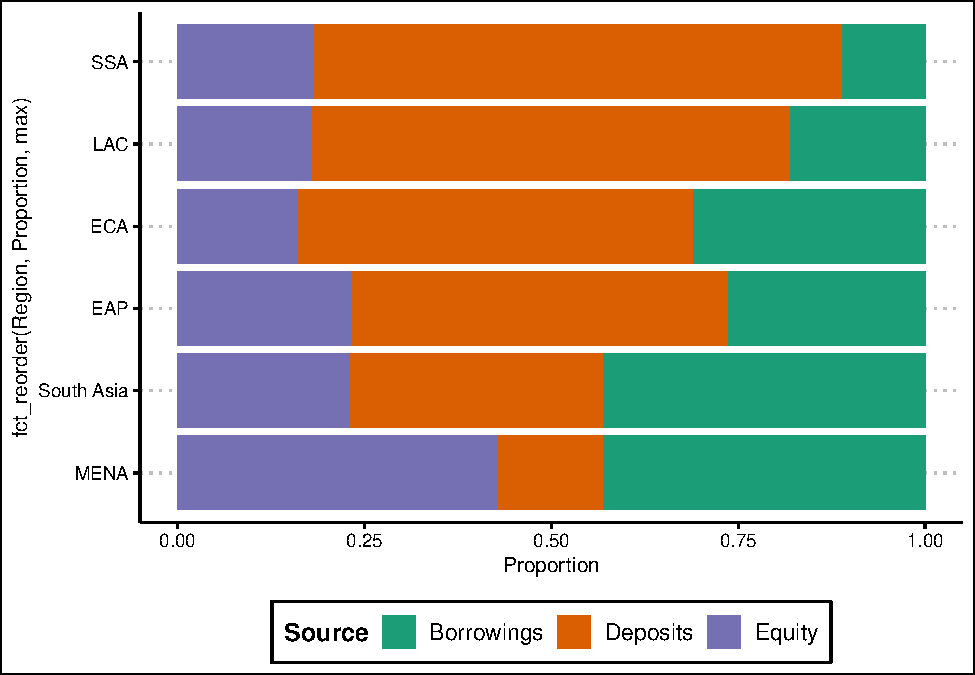
\includegraphics{_main_files/figure-latex/unnamed-chunk-5-1.pdf}
\caption{\label{fig:unnamed-chunk-5}Funding structure of MFIs Across the Globe by Region (2015)}
\end{figure}

Although the transformation of NGOs has its merits, most MFIs have still not transformed\autocite{d2017ngos}. Therefore, a key output of the proposed study will be the motives behind some MFIs transforming while other MFIs retain the NGO model. The current literature has been overly concerned with the transformed MFIs and not addressed this issue. Even among the transformed MFIs, researchers have not uncovered the drivers of the decision by MFIs to transform and the necessary preconditions for transformation. The existing research takes for granted that MFIs transform to be sustainable. Given the benefits of transformation touted in the numerous studies, then most MFIs should have already transformed.

Moreover, as \textcite{morduch2019challenges} argues, if there is no trade-off between financial performance and social performance of transformed MFIs, then NGOs would not exist. However, this is not the case. It appears, therefore that some additional factors influence the decision by MFI to either transform or retain the NGO model. As noted, there is no conclusive evidence on the effects of MFI transformation on their performance. These contradicting results could be because of numerous unknown reasons. It is in order, therefore, to establish the factors that influence the sustainability and outreach of transformed MFIs. Similarly, establishing the factors that moderate the relationship between capital structure on the one hand and the financial performance and social performance of MFIs in Africa will be a novel contribution to the research.

Recent literature also suggests that the performance of MFIs is dependent on the broader macroeconomic conditions as well \textcite{ahlin2011does}, and is country-specific \autocite{d2017ngos}. Thus, in the analysis of the institutional transformation of MFIs, cross-country and regional differences must be factored in. However, most studies have not considered the cross country and regional variations. Failure to consider regional disparities means that the extant research fails to capture local contextual peculiarities.

These regional differences motivate the choice of MFIs in Africa as the unit of analysis. By focusing on Africa, the study will isolate the regional and country heterogeneity of the effects of transformation, an issue that could have affected the results of research based on pooled global datasets. Thus, the output of the study will be unique to Africa and therefore more actionable. To sum up this section, the proposed study significantly extends the existing literature on MFI transformation. The next section outlines the purpose statement.

\hypertarget{purpose-statement}{%
\section{Purpose Statement}\label{purpose-statement}}

\noindent The primary aim of this proposed research is to evaluate how the the transformation of MFIs in Africa impacts their financial and social performance.

\hypertarget{research-questions}{%
\section{Research Questions}\label{research-questions}}

\noindent The study specifically seeks answers to the following research questions.

\begin{enumerate}
\def\labelenumi{\arabic{enumi}.}
\tightlist
\item
  Why do some MFIs in Africa transform into the commercial model while others retain the NGO Model?
\item
  To what extent has the institutional transformation of MFIs in Africa affected financial inclusion?
\item
  After transformation, what factors explain the joint level of sustainability and outreach by MFIs in Africa?
\item
  What are the factors that influence the choice of financing sources by transformed MFIs in Africa?
\item
  How is capital structure related to the performance of transformed MFIs in Africa?
\end{enumerate}

\hypertarget{significance-of-the-study}{%
\section{Significance of the Study}\label{significance-of-the-study}}

\noindent In pursuing the stated objectives, this study will fill a theoretical deficiency in the capital structure of quasi-commercial organisations that have a social dimension of value. The context of shareholder and debtholder primacy was the foundation of the development of capital structure theories. Arguments from this genesis of capital structure theories have failed to factor in corporations with extra dimensions of value, such as the achievement of social goals. As a case in point, \texttt{Modigliani\ and\ Miller} capital structure theory may not be entirely applicable to MFIs where value also has a social facet. In the Modigliani and Miller capital structure theory, the value of a firm is the sum of equity and debt components in the capital structure of a corporation. The value of a company is an increasing function of the debt proportion of capital structure up to the point where the costs of financial distress outweigh the benefits of the interest tax shield.In the process, the study will also fill an empirical deficit on the relationships between capital structure on the one hand, and financial performance, social performance, and efficiency of transformed MFIs in Africa. The empirical output has implications on policy direction relating to MFIs in Africa.

The study also has a variety of policy implications. These policy implications are related to the research objectives. For instance, what are the factors that drive MFIs to transform or fail to transform? The answer to this question would inform the crafting of policy if transformation is indeed desirable. Moreover, what are the drivers of financial inclusion, outreach, and sustainability of MFIs after the transformation? Lastly, what are the determinants of the choice of financing sources? It is worth noting that if the drive for institutional transformation is to achieve the desired effects, then the change in the MFI funding structures must not compromise the achievement of social objectives. If the conversion of MFIs negatively affects social performance, there would be no way to justify the transformation of MFIs. If indeed the transformation of MFIs was meant to improve their sustainability, this must not be to the detriment of social performance.

Also, if the transition results a decline in social performance, then the transformation could be treated as the transition point of transformed MFIs into the mainstream banking system \autocite{kent2013bankers}. It is crucial therefore to investigate the outcomes of the change to inform the design of a framework that would not expose the poor and financially excluded to the same level of exclusion by the financial system that MFIs ought to address. Doing this would be tantamount to allowing MFIs to use the underprivileged as a ladder to climb into the mainstream system, and abandoning them shortly after, which raises ethical questions.

Similarly, the identification of factors that influence the choice of financing structures has implications for the design of policies aimed at the capital market. For the same reasons, the identification of factors that influence the social performance of transformed MFIs will also be useful, not just for policy design, but also for managerial decision making. Also, the calibration of a mix of debt and equity for transformed MFIs that optimises financial and social performance will inform both policy-making and managerial decision making.

Finally, the efficiency of MFIs is a significant determinant of both the financial and social performance of MFIs. According to the efficiency theory, the positive relationship between concentration and profitability is indicative of the tendency of firms that are efficient to be successful and hence dominant in their industries \autocite{lipczynski2005industrial}. Efficiency gains could result from economies of scale and cost-saving schemes initiated by the management. Enhanced efficiency by MFIs is, therefore desirable. However, the efficiency of MFIs should encompass both financial and social dimensions. The entry of commercial sources of capital may affect the both the financial and social efficiency of MFIs in line with agency theory. It is therefore vital to establish the relationship between capital structure and efficiency to inform both the management and stakeholders of the dynamics in the MFI sector regarding effectiveness in the new era of commercial funding.

\hypertarget{outline-of-the-study}{%
\section{Outline of the Study}\label{outline-of-the-study}}

\noindent The remainder of the study will be structured as follows. Chapter two locates microfinance in the financial intermediation space and traces the genesis and evolution of the transformation. Chapter three lays out the theoretical framework of the study, focusing on the agency theory and profit incentives, capital structure theory, and the institutional theory. The subsequent five chapters each delves into one research question, laying out the methodologies applied and the results. The last chapter concludes.

\hypertarget{cites-and-refs}{%
\chapter{Financial Intermediation and the Transformation of Microfinance Institutions: A synthesis}\label{cites-and-refs}}

\chaptermark{Transformation of Microfinance: A Synthesis}

\minitoc 

\hypertarget{introduction}{%
\section{Introduction}\label{introduction}}

\noindent This chapter provides contextual information that lays the foundation for the review of the empirical literature on the transformation of MFIs. The chapter starts by introducing financial intermediation and then locates microfinance in the financial intermediation space. The section subsequently presents an overview of the evolution of microfinance and the drift towards the conversion of MFIs from the NGO model to the commercial model. Next, the chapter presents the extent of the transformation of MFIs in selected African countries, including the manifestation of the transformation of MFIs. The section concludes by outlining the challenges that MFIs face in the transformation process.

\hypertarget{need-for-financial-intermediation}{%
\section{Need for Financial Intermediation}\label{need-for-financial-intermediation}}

\noindent Financial intermediaries play a central role in the economy (Kodres, 2017). They contribute to economic development by transforming the maturity and liquidity of assets, providing leverage, and transferring credit risk (Uddin et al., 2014, Valickova et al., 2015, Gajjala and Gajjala, 2016). By channelling excess funds from the individuals and institutions to those that have deficit savings the intermediaries resolve the problem of information asymmetry between lenders and borrowers and cut costs associated with the duplicated screening of potential borrowers (Greenbaum et al., 2015).

Typical services provided by financial intermediaries include brokerage and qualitative asset transformation \footnote{Examples of brokerage services include transaction services (e.g.~deposits and cash transfer), financial advice, screening, origination, and funding (loan issuance). On the other hand, qualitative asset transformation involves monitoring, guaranteeing, liquidity creation and the management expertise associated with these activities. See GREENBAUM, S. I., THAKOR, A. V. \& BOOT, A. 2015. Contemporary financial intermediation, London, Academic Press. for more details of the services offered by financial intermediaries.} (Greenbaum et al., 2015, Gobat, 2017). Financial intermediation allows individuals to make long-term consumption and investment decisions and overcome liquidity constraints associated with the uncertainty of income streams (Greenbaum et al., 2015). In doing so, financial intermediaries allow for the efficient allocation of capital that improves total factor productivity (International Monetary Fund (IMF), 2017) which contributes to economic growth (Chang et al., 2017). Also, financial intermediaries create money and act as conduits for the transmission of monetary policy (Greenbaum et al., 2015). In turn, financial intermediaries generate revenue primarily from the spread between lending and deposit rates, the sale of securities and fees from customer services (Cosci et al., 2015).

Commercial banks are among the most prominent financial intermediaries. However, there exists a wide array of alternative financial intermediaries which offer services like those of commercial banks, yet they are not commercial banks. The Financial Stability Board (FSB) classified such institutions as shadow banks \footnote{FSB definition of shadow banking is ``the credit intermediation involving entities (fully or partially) outside the regular banking system.''} (Financial Stability Board, 2017) . Examples of shadow banks include credit unions, mutual funds, broker-dealers that finance their assets using repos, insurance companies, finance companies, and MFIs. Central banks do not regulate most shadow banks. For this reason, most shadow banks cannot, for example, get emergency loans from the central bank. Also, deposit insurance does not cover most deposits of shadow banks (Kodres, 2017).

By their very nature and scale, shadow banks were not a priority for regulators and policymakers until after the 2007 global financial crisis triggered by defaults in the shadow banking system. It was after the crisis that researchers and policymakers realised that the shadow banking sector could be endogenously destabilising, especially with the interconnectedness of the modern global financial system (FSB, 2017). Shadow banks have since been subject to increased regulatory oversight (Adrian and Narain, 2017).
Despite the benefits conferred by the access to and use of financial services, financial intermediation also has its drawbacks. For instance, the profit margin enjoyed by the intermediary has the net effect of increasing the cost of borrowing and reducing the rate of interest on deposits. Consequently, disintermediation, the reliance by large borrowers on direct rather than indirect finance, is gaining popularity (Greenbaum et al., 2015).

Furthermore, the mainstream financial intermediaries like commercial banks face hurdles in availing financial services to the poor and the financially excluded (including the business ventures these parties pursue \footnote{Research indicates that small businesses ran by the poor (mostly agricultural-based microenterprises), and SMEs, experience financial exclusion, especially lack of access to credit to finance their operations as well as access to savings products.}). At the base of the pyramid, information opaqueness of the clientele poses a monumental challenge against the provisioning of financial services. For instance, deprived rural dwellers often lack credit histories, a result of being geographically isolated, and financially excluded for prolonged periods (Alimukhamedova et al., 2015).

Also, individuals in this market segment often lack collateral to secure credit (Brière and Szafarz, 2015). Besides, the tiny amounts of cash transacted at the bottom of the pyramid result in substantial diseconomies of scale (Abate et al., 2014, Cobb et al., 2016). Moreover, the products and services offered by mainstream banks often do not meet the immediate needs of the poor (Gajjala and Gajjala, 2016). Lastly, difficulties in contract enforcement, especially in low-income countries, exacerbate the situation (Klapper and Singer, 2014). Thus, at the bottom of the pyramid, the problem of information asymmetry, lack of tangible assets, and the small scale of operations manifest more acutely.

In the same vein, indigent and financially excluded clients exhibit low levels of literacy and a high incidence of extreme poverty. Consequently, the level of financial illiteracy at the base of the pyramid is similarly high that it hinders the utilisation of financial services, even when they are available (Engström and McKelvie, 2017). Thus, until the advent of microfinance, most of the Microfinance (MF) market segment was not catered for by the mainstream financial intermediaries. Researchers still find that most of the persons in this segment suffer from financial exclusion (Kota, 2007).

Before the entry of microfinance, informal financing arrangements, like direct financing between family members and friends, family and community merry-go-rounds, self-help groups (SHGs), neighbourhood retail traders and shylocks often filled the void (Klapper and Singer, 2014). These informal mechanisms and alternative formal financial intermediaries like Microfinance Institutions (MFIs) and other shadow banking institutions remain the significant players in offering financial services to the poor and the financially excluded (Klapper and Singer, 2014). In this context, the next section highlights the rise of MF, a significant part of the shadow banking system committed to availing financial services to the poor and the financially excluded.

\hypertarget{rise-of-microfinance}{%
\section{Rise of Microfinance}\label{rise-of-microfinance}}

\noindent As already noted, the social and economic empowerment of the poor and the financially excluded, particularly among women and rural dwellers are central to the validation of microfinance (Engström and McKelvie, 2017). The broader view remains that poverty reduction is not only desirable but also has positive externalities. It is in with this hindsight that, in awarding the Nobel Peace Prize to Mohammed Yunus and the Grameen Bank, the Nobel Committee cited the link between poverty reduction and peace (``Announcement of the 2006 Nobel Peace Prize,'' 2006).

It is paramount to distinguish between MF as a concept, and in reference to the providers of MF services. As a concept, MF refers to the provision of financial services to the financially excluded sections of the population. A large body of institutions and individuals provide the services, including but not limited to MFIs, public and private commercial banks, NGOs, civil society organisations of public interest (OSCIPs). Other providers include international development organisations, commercial retailers, post offices, credit unions, and informal money lenders (Ledgerwood and White, 2006, Marconatto et al., 2016). Nevertheless, the provision of MF has received both support and condemnation from researchers and policymakers.

Despite the reservations about MF, researchers, and policymakers deemed it a useful tool to avail financial services to individuals previously excluded from the financial system (D'Espallier et al., 2017b). Moreover, given the limitations of the formal banking system, advocates of financial inclusion pushed for microfinance as the viable alternative to efficiently reach the poor and the financially excluded (Chester et al., 2016). Unlike mainstream financial institutions, MFIs reach the poor through innovative approaches such as group lending, regular repayment schedules, progressive lending (dynamic incentives), and collateral substitutes (Bhuiyan et al., 2016). MFIs also focus more on women and people living in rural areas (Ghosh, 2013).

The model followed by the modern microfinance business is attributable to Mohammad Yunus and Grameen Bank operating in Bangladesh from the mid-1970s (Ghosh, 2013). After the Yunus and Grameen Bank microfinance model gained traction, the number of MFIs operating has exploded across the globe. Table 2.1 gives the current estimated size of the microfinance market based on data from the MIX pooled database. However, not all MFIs avail their data to the database, and hence the data is an under-representation of the scale of the industry.

Initially, researchers and policymakers hailed MF as the magical apparatus to resolve the problems of development and poverty (Ghosh, 2013). Researchers have associated MF with increased investment by pre-existing business ventures (Newman et al., 2017) and a reduction in gender inequalities (Shahriar and Garg, 2017, Newman et al., 2017, Mafukata et al., 2017, Zhang and Posso, 2017). Further, there is a direct relationship between MF and household welfare (Meador and Fritz, 2017, You, 2013), purchasing power and employment rate (Lopatta and Tchikov, 2016, Raihan et al., 2017). Also, MF supporters contend that it enables families to cope with the effects of climate change (Fenton et al., 2017) and also deal with the shocks arising from natural disasters (Calis et al., 2017).

Furthermore, researchers have found that access to microcredit leads to higher business start-ups while increasing the profitability of existing businesses (Klapper and Singer, 2014). Other social indicators that have a positive relationship with MF include the savings rate among the poor, health, child mortality, education, and financial inclusion (Shahriar and Garg, 2017, O'Malley and Burke, 2017). At the macro-level, researchers have found an inverse relationship between the size of the MF in a country and poverty levels (Ahlin et al., 2011). Also, research indicates that MF significantly influences economic development by directly increasing the purchasing power of beneficiaries and indirectly via improved capital accumulation and increased employment rate (Lopatta and Tchikov, 2016, Raihan et al., 2017). Given these findings, it was not a surprise that the UN declared 2005 the international year of microcredit followed by the award of the Nobel Peace Prize to Muhammad Yunus and the Grameen Bank in 2006.

\newpage

\begin{landscape}\begin{table}
\centering\begingroup\fontsize{8}{10}\selectfont

\begin{tabular}{lrrrrrrrrr}
\toprule
Region & FSPs & Borrowers\_000 & \%\_Borrowers & Gross\_Loans\_000 & \%\_Gross\_Loan & Depositors & \%\_Depositors & Desposits\_USDMillions & \%\_Deposits\\
\midrule
Africa & 193 & 5778 & 0.05 & 8490 & 0.09 & 17298 & 0.18 & 9212 & 0.16\\
EAP & 136 & 16258 & 0.14 & 15064 & 0.16 & 16118 & 0.16 & 7687 & 0.13\\
ECA & 136 & 3083 & 0.03 & 9900 & 0.11 & 5091 & 0.05 & 7664 & 0.13\\
LAC & 345 & 22495 & 0.19 & 38843 & 0.42 & 23709 & 0.24 & 27293 & 0.46\\
MENA & 27 & 2148 & 0.02 & 1353 & 0.01 & 465 & 0.00 & 251 & 0.00\\
\addlinespace
South Asia & 196 & 66929 & 0.57 & 18794 & 0.20 & 35109 & 0.36 & 6886 & 0.12\\
Grand Total & 1033 & 116691 & 1.00 & 92443 & 1.00 & 98420 & 1.00 & 58994 & 1.00\\
\bottomrule
\end{tabular}
\endgroup{}
\end{table}
\end{landscape}

\newpage

However, some researchers view MF as a double-edged sword that is beneficial to individuals and society but also has some unintended consequences (Ganle et al., 2015, Van Rooyen et al., 2012). For example, Ganle et al.~(2015) and Van Rooyen et al.~(2012) found that while some women indeed get empowered as a result of access to credit, most have little control over the subsequent spending. A significant proportion suffers harassment from MF agents' for failing to repay the loans. These coercive loan recovery practices ignited the ``no pago'' protests movement in Nicaragua \footnote{In mid-2008, a movement called ``movimiento no pago'' (Spanish for ``a movement for non-payment of loans'') led by over-indebted farmers in Nicaragua protested MFIs operating in the area. The protests were triggered by the arrest of MFI debtors in default. The movement gained political support, including from the president of Nicaragua, Daniel Ortega. In the end, laws were passed that favored the indebted, including the fixing of interest rates at 16\% and an extension of loan recovery periods.} and led to several incidences of suicide by MF loanees in Andhra Pradesh , India \footnote{In 2010, the government of the state of Andhra Pradesh, India, passed an ordinance to protect borrowers from harassment from MFI agents. This came in the backdrop of suicides committed by some indebted MFI clients, protests by MF borrowers, and reports of increasing violence targeted at MFIs. The Andhra Pradesh Microfinance Institutions (Regulation of Money Lending) Ordinance, 2010 requires all MFIs to register with the state government, specify the areas they operate in, the rate of interest and their system of operation and loan recovery. The law also set stiff penalties for coercive loan recovery, prohibited multiple loans to the same borrower, and capped interest chargeable not to exceed the principle loan amount GHOSH, J. 2013. Microfinance and the challenge of financial inclusion for development. Cambridge Journal of Economics, 37, 1203-1219.} (Bastiaensen et al., 2013, Wright et al., 2016). These MF crises resulted in intervention by authorities in both countries, lifting the veil on the dark side of MF. Similarly, although MF does allow women to raise their income levels, in some instances, it has also led to an increase in domestic conflict (Salia et al., 2017).

Furthermore, Newman et al.~(2017) uncovered an insignificant link between MF and improvements in consumption, although spending on business-related investment does rise. Shahriar and Garg (2017) also find that the relationship between MF and both business size and profitability only holds in the long run, calling into question the benefits of the short-term loans offered by MFIs. Research has concluded that MF does not often reach the poorest, as they get crowded out by the better-off clients (Abeysekera et al., 2014). Sir Fazle of BRAC, an MF operating in Bangladesh, attributes the failure by the poorest to borrow on stigmatisation by the society, where ``fellow villagers viewed them (the poor) as hopeless cases''(Zulfiqar, 2017b).

Likewise, Aguilera et al.~(2017) posit that in the short term, some clients of MF benefit more than others. For example, compared to men, women customers of MF get lower profits from their MF funded businesses. On the same line, older women generate fewer profits compared to younger women. Furthermore, Akotey and Adjasi (2016) conclude that the benefits of microcredit are enhanced or sustained only when coupled with microinsurance. Thus, as Onyuma and Shem (2005) note, microcredit alone cannot cure the ills associated with financial exclusion and poverty. The implication is that MF should look beyond microcredit by offering other financial products. Recent developments in MF have seen the introduction of savings products, microinsurance, pension products and cash transfer services (Chandrasekhar and Anantharaman, 2015).

However, there is also a substantial body of research that disputes the benefits of MF (Bateman, 2010a, Bauchet and Morduch, 2013). For instance, the opponents of MF contend that it does not fund genuinely entrepreneurial activity but instead focuses on small retail operations that neither allows the poor to escape poverty nor even have a significant effect on economic growth (Aguilera et al., 2017). MF leads to a glut in the market for similar products by the poor that causes default and overindebtedness. Moreover, the enterprises funded through MF often do not develop linkages with the formal economy, thus inhibiting the development of synergies in productive activities which further limits innovation and productivity improvements (Ghosh, 2013). Furthermore, some researchers posit that MF does not boost employment and education among the rural poor (Bauchet and Morduch, 2013). Others link micro-credit to increased child labour (Hazarika and Sarangi, 2008), increased gender inequalities in access to finance (Zulfiqar, 2017a), and reduced entrepreneurial spirit among the poor (Field et al., 2013).

Still, some researchers are chiefly concerned with the high-interest rates charged by MFIs and inappropriate lending practices that fail to account for the social, cultural, and economic context of the target clients (Chester et al., 2016). The basis of the lending practices of modern MF is the logic of western capitalism that stresses individual wealth accumulation. By contrast, poor communities emphasise economic processes (not outcomes), shared roles, survival, and varied economic activities which acts as a collective safety net (Chester et al., 2016).

Researchers have thus argued an over-emphasis on individual achievement, and the advent of group lending is likely to set back social cohesion as members segregate themselves into groups, directly or indirectly monitor each other and impose sanctions on loan defaulters (Chester et al., 2016). Moreover, the logic of western capitalism that forms the basis of MF degrades community ownership and control over assets. Finally, researchers have argued that the narrow definition of MF may be detrimental to the broader development agenda in poor communities, including the provision of physical infrastructure, security, education and health services (Ghosh, 2013).

Furthermore, some researchers claim that the high-interest rates charged by MFIs are unaffordable by clients, and only serve to trap them in a debt cycle (Wright et al., 2016). Researchers have likened the high-interest rates charged by MF to a poverty penalty, raising ethical concerns (Chang et al., 2017). Moreover, a substantial number of MF clients get credit from several MFIs. The subsequent confiscation of assets further lowers social status (Paprocki, 2016).

Microcredit was meant to promote the welfare of the poor by funding entrepreneurial activity. However, some researchers have pointed out that it is not reasonable to presume that all poor people desire to or have the capacity to engage in such activity. As Ghosh (2013) asserts, some MF clients pretend they want credit to fund microenterprises but use the cash for subsistence, health care, and school fees. Some even use the loans to buy durable goods like televisions. Scholars assert that it is simplistic to assume that the lack of access to capital is the primary reason behind limiting the engagement of poor people in entrepreneurial activity. As Kimmitt and Munoz (2017) note, capital is a necessary but not sufficient condition for innovation and the uptake of entrepreneurial economic activity, even among the poor. There are additional resources that are complementary to money such as human capital, social capital, and effective institutions that are lacking in most impoverished communities.

Moreover, even in cases where all these preconditions are present, they may not be enough to trigger structural changes necessary for the reduction of poverty --- the environment where these institutions operate matters. Thus, the evaluation of the success or failure of MF must take into account the context of the situation, such as political freedom, economic facilities, social opportunities, transparency guarantees, protective security (Sen, 2014), and even cultural norms (Shahriar and Garg, 2017). It is against this backdrop that some studies recommended a reexamination of the MF business model and called for better regulation of the industry (Johnson, 2013, Ghosh, 2013). Without reforms, conclude Chester et al.~(2016), ``the MF industry could not only ruin the lives of many borrowers but could also ruin itself.''

The debate surrounding the contradictory results arising from MF interventions has preoccupied researchers in MF for a prolonged period. Researchers have pointed to the weaknesses in the numerous methods used to evaluate the performance of MFIs (Awaworyi Churchill and Nuhu, 2016), institutional factors (Kimmitt and Munoz, 2017), and diverse cultural norms (Shahriar and Garg, 2017) for the discrepancies.

\hypertarget{bankrolling-mf-the-place-of-subsidies-and-grants}{%
\section{Bankrolling MF: The Place of Subsidies and Grants}\label{bankrolling-mf-the-place-of-subsidies-and-grants}}

\noindent Before the advent of transformation, most MFIs relied on donor grants and subsidies to finance their operations. Grants are private funds from individuals and corporations, whereas subsidies are funds provided by the government to organisations that benefit the public. Although data is hard to come by, some studies estimate that only 23\% of MFIs across the globe operate without subsidies and grants (D'Espallier et al., 2013).

Consultative Group to Assist the Poor (CGAP) (2017) estimates that both public and private donors provided US\$ 2.9 Billion in funding to MFIs in 2013. In comparison, the funds raised by MFI through the sale of debt and equity instruments, and guarantees amounted to US\$ 13.8 Billion, US\$ 3.7 Billion and US\$ 1.4 Billion, respectively. Different funding agencies tend to use various instruments to support MF activities. Bilateral agencies and foundations, for example, mostly use grants as opposed to development finance institutions that typically use debt, only using equity and guarantees sparingly. Multilateral agencies mainly give loans to governments and grants to MFIs for technical assistance. Government mostly offer subsidies to MFIs (Consultative Group to Assist the Poor (CGAP), 2017).

The provision of the grants and subsidies allowed MFIs to reach the poor without the pressure to generate profits to sustain their operations (D'Espallier et al., 2013). Likewise, subsidies are useful for setting up start-ups and risky ventures where alternative funds are not available (Bogan, 2012). The subsidies and grants thus played a significant role in the setting up of the MF industry when the mainstream financial intermediaries did not consider it a viable business venture and commercial funding were unavailable.

As Hudon (2010) note, the presence of subsidies and grants allows the MFIs to charge lower interest rates. However, other researchers posit that MFIs could still manage to charge low-interest rates if they manage their expenses better, even in the absence of subsidies. Further, given that some grants and subsidies support capacity building of MFI staff, the presence of subsidies could indicate better management and operational practices, which have implications on both social and financial performance of the MFIs. On the contrary, some scholars argue that subsidies may encourage lax management leading to inefficiencies (Ghosh, 2013).

Researchers also argue that subsidies and grants serve to repress the rationing role played by interest rates (Hudon, 2010). Interest rates are not only a source of revenue for financial intermediaries but also ensure that only viable projects access financing. It means that a project must generate a rate of return to service the interest payments and make sufficient returns for the investors. The presence of subsidies and grants means that MFIs may fund poor quality projects which reduces social welfare in the aggregate. As Kota (2007) argues, the subsidised MFIs also crowd out the efficient financial intermediaries. In this respect, Ghosh (2013) and Bayai and Ikhide (2016) call for the design of smart subsidies that do not distort the market but rather serve to strengthen the institutions.

Furthermore, the presence of subsidies in MFIs may push out informal credit suppliers. Although the discussion around informal money lenders is mainly adverse, they still form a significant source of credit for poor households (Klapper and Singer, 2014). The conversation around offering financial services to the poor should then be about how MF can serve to supplement, rather than completely replace the informal financial sector. Instead, the western driven research discourse around MF and poverty dwells on the need to replace the inefficient informal financial systems with an efficient, formal system modelled on western capitalist thinking. The direction taken by researchers fails to reflect on the social-cultural inclinations of the members of poor communities (Chester et al., 2016) and rules out the existence of alternate ``systems of exchange'' beyond the price-driven model dominant in economics and finance literature (Biggart and Delbridge, 2004).

Lastly, subsidies diminish incentives by MFIs to develop and offer new products. If financing from subsidies is guaranteed, then MFIs lack the motivation to diversify their revenue sources. Indeed, before transformation, most MFIs offered only microcredit (Cozarenco et al., 2016) although legal restrictions did not allow MFIs to provide some products, for instance, savings. After the transformation, the range of the services provided by MFIs expanded. The expansion of the services provided by MFIs post-transformation is, to some extent, the evidence against the reliance on subsidies and grants by MFIs.

\hypertarget{alternatives-and-complements-to-mf}{%
\section{Alternatives and Complements to MF}\label{alternatives-and-complements-to-mf}}

\noindent Based on the criticism of microfinance, the financial system has witnessed the development and adoption of new strategies to reach the poor. However, these new approaches are not exactly meant to replace MF, but rather to complement it by bridging its shortcomings. A prominent case is the use of mobile money which has proved to be a useful tool for expanding financial inclusion. In Kenya, for example, M-Pesa, M-Kopa, and M-Shwari have contributed positively to financial inclusion by allowing the poor to pay bills, save, transfer and receive money conveniently at a relatively low cost (Klapper and Singer, 2014, Ndung'u et al., 2017). Numerous financial institutions and Fintech companies across the globe have since developed and adopted the mobile money platform. MFIs have espoused mobile money and web technologies to reach their clients (Griffoli, 2017, Ouma et al., 2017).

``Graduation'' program is an alternative scheme where indigent persons are provided with an asset, for example, cattle and offered training in livestock management \footnote{A graduation program could also involve providing a poor person with seeds, fertilizer, crop insurance and training in plant husbandry. The resources are provided on loan to be repaid at an agreed rate of interest. The One Acre Fund, an NGO based in Eastern Africa, has experimented with this model.} . Results from random controlled trials (RCT) indicate that such ``graduation'' programs are more successful than the provision of microcredit alone. According to Bishop and Rodríguez (2017), graduation programs result in more wealth and raises the demand for food and other durable goods among the poor people participating in the program. However, the programs are not only expensive but also hard to implement in urban settings where agricultural activity is limited. Furthermore, such wealth generating programs, make products such as savings and insurance even more useful to clients (Cozarenco et al., 2016).

Finally, governments and other organisations in several developing countries give conditional cash transfers to individuals who meet specific criteria (Rawlings and Rubio, 2005, Tadesse and Zewdie, 2019). For example, a scholarship program operational in Cambodia make cash transfers to households contingent upon the enrollment of children in school (Ferreira et al., 2017). In Kenya, there is a program that awards specified cash awards to citizens above 70 years of age living in poverty (Sandra and Juan, 2017). However, in addition to implementation challenges, conditional cash transfers are affected significantly by political leadership, program administration and even natural disasters (Rodgers, 2014). Moreover, conditional cash transfers have an incentive effect on individuals; where non-poor individuals change their behaviour to receive benefits meant for the poor (Brown et al., 2017). Also, there is mixed evidence regarding the efficacy of cash transfer programs (Sandra and Juan, 2017).

\hypertarget{mf-to-financial-inclusion-the-paradigm-shift}{%
\section{MF to Financial Inclusion: The Paradigm Shift}\label{mf-to-financial-inclusion-the-paradigm-shift}}

\noindent Recent developments have seen researchers and policymakers start to rethink the central place of MF in achieving financial inclusion (Cobb et al., 2016). The new financial inclusion paradigm recognises that MF is just one element of a broader set of strategies for financial sector development. They call for the development of long-term policies that would enable the players in the financial system beyond MF to avail their services to the poor and the financially excluded (Ghosh, 2013). Thus, although MF has made a valuable contribution to financial inclusion, these researchers argue that a multifaceted approach involving all the alternative providers of financial services could achieve better results (Taylor, 2012). In this respect, almost all financial intermediaries, including commercial banks, have to some extent developed products that suit the needs of the indigent and other financially excluded individuals (Johnson, 2013, Ndung'u et al., 2017).

Recommendations to achieve financial inclusion include the development of policies to keep interest rates low and keeping in check to destabilising capital flows (Lund and Harle, 2017). Also useful are legal, fiscal and monetary mechanisms to influence the flow of credit to the poor and the financially excluded. These researchers contend that the achievement of these objectives would require some form of subsidies and grants (Ghosh, 2013).

The financial inclusion paradigm has resulted in heightened competitive pressure among financial intermediaries. Increased competition is forcing MFIs to pay attention to the minimisation of operational costs to boost efficiency. In this respect, MFIs are seeking economies of scale (by netting in more customers) and economies of scope (by rolling out more products beyond microcredit), and leveraging on mobile and web technology and agents in place of brick and mortar branches (Muriu, 2016). Overall, the competitive pressure, the rise of the neoliberal political-economic paradigm, legal requirements and pressure from donors has resulted in some MFIs transforming from NGOs to commercial entities (Muriu, 2016, Kar, 2016). The transformation of MFIs is changing the financial intermediation landscape, even for the indigent clients. The conversion of MFIs is detailed next.

\hypertarget{transformation-of-mfis}{%
\section{Transformation of MFIs}\label{transformation-of-mfis}}

\noindent At the initial stages of MF development, most MFIs operated as NGOs, raising capital mainly from the public and private donations. However, starting in 1992, some MFIs have converted to commercial entities sourcing funds in the capital market and emphasising profitability and sustainability, simultaneously with the pursuit of their social mission of serving the poor. Bateman (2010) traces the momentum for the transformation of MFIs from NGOs to commercial entities to the rise of neo-liberalism in the mid-1970s. Core to the neo-liberal paradigm was the need for all institutions operating in the economy to be financially self-sustainable. Thus, economic liberalisation, commercialisation, and privatisation of public enterprises characterised the neo-liberalism wave.

In developing countries where most of the formal MFIs operate, the IMF and the World Bank induced structural adjustment programs (SAPs) were the significant indicators of the global reach of neo-liberalism. SAPs were designed to allow the economies of target countries to be more market-oriented (Easterly, 2003). Similarly, the World Bank, USAID, and other donor agencies pushed for the transformation of MFIs with the aim of expanding MFI outreach without the need for subsidisation (Ghosh, 2013). For MFIs, the adjustments meant that the interest rates charged were to be determined by market forces in place of the below-market, subsidy-supported rates (Bateman, 2010a). Similarly, MFIs that undertook the transformation worked to increase the client base to lower the fixed cost per client and offered incentives to senior managers, including significant ownership stakes in the MFIs (Lauer, 2008). In some other countries, for example, Georgia , legal changes forced MFIs to transform into commercial entities \footnote{Legislation enacted in Georgia required that all NGOs cease engaging in MF activities by December 31, 2007 LAUER, K. 2008. Transforming NGO MFIs: Critical ownership issues to consider, New York, Consultative group to assist the poor (CGAP)}.

With neo-liberalism, most of the donor organisations that channelled funding to MFIs also pushed for the commercialisation of the MFIs. To date, a substantial number of MFIs have converted to commercial entities. Notable though is that most MFIs have survived the neo-liberal onslaught and still operate as NGOs (D'Espallier, Goedecke, Hudon, \& Mersland, 2017). The shift from the NGO model to the commercial model has several implications. First, researchers point out that the profit motive has the potential to shift the focus of MFI's away from their social mission of serving the poor and the financially excluded to the emphasis on financial returns. ``Mission drift'' is the term used to describe this potential change in business model focus (Mersland \& Strøm, 2010).

Similarly, the departure from predominant reliance on donor funding to commercial funding has implications from the agency theory perspective. In this respect, agency conflicts may manifest between shareholders on the one hand, and the management, debt-holders, private and public donors on the other, and this influences the performance of the MFI (Fama, 1980). Also, agency conflicts have the potential to affect the funding structure and performance of MFIs (Berger and Bonaccorsi di Patti, 2006, Le and Phan, 2017). Consequently, researchers have raised questions regarding how well MFIs have balanced financial self-sufficiency and the pursuit of social goals after the shift to the new business model. It is upon this basis that the world bank launched an equity fund to support MFIs to meet the costs of the transformation and to safeguard their social mission (Frank et al., 2008).

\hypertarget{schools-of-thought-on-the-transformation-of-mfis}{%
\section{Schools of Thought on the Transformation of MFIs}\label{schools-of-thought-on-the-transformation-of-mfis}}

\noindent As noted, state agencies, donor agencies, and philanthropists were the most significant sources of funding for MFIs (Ledgerwood, 1998, Ledgerwood and White, 2006). The initial thrust for MF arose from the desire to lift the billions of people that languished in poverty, mostly in third world countries. Availing credit to the poor was and is still seen as an essential first step towards breaking the vicious cycle of poverty. However, some researchers contest this view (Bateman, 2010a, Adams and Vogel, 2016, Onyuma and Shem, 2005). Thus, MFIs were established solely to tackle human misery that arose from the scourge of poverty.

In the circumstances that motivated the establishment of the first MFIs like Grameen, the profit motive was ethically incompatible with the MF agenda (Ghosh, 2013, La Torre, 2006) due to the ethical concern around the ``financialization'' of poverty (Mader, 2016). Yunus had emphasised the need for MFIs to maintain low interest rates, in contrast with the usurious rates charged by moneylenders in rural Bangladesh that Grameen Bank and other MFIs were supposed to replace (Bateman, 2010a). Consequently, MFIs set the interest rate below the market rate. Accordingly, MFIs operated as NGOs, focusing more on their social mission of serving the poor and the financially excluded than the generation of profits. The welfare approach to the provision of MF underpinned this model.

Proponents of the welfare approach argued that MFIs could attain their social mission without being financially self-sufficient (Kodongo and Kendi, 2013a). The welfare approach further holds that the social purpose of MFIs is paramount and incompatible with financial sustainability. To the researchers who subscribe to this school, financial viability (commercial orientation) and an emphasis on the social mission (development positioning) of MFIs are different approaches that have different aims and motives (Toindepi, 2016). They cite ample body of empirical studies that uncover a decline in social performance by MFIs that have to pursue both the profit motive and the social mission (i.e., transformed) in support of their view. Bos and Millone (2015) and Mia and Lee (2017), for instance, find that capital market funding is subject to mission drift, the evidence against the feasibility of the institutional transformation of MFIs.

Over time, however, some researchers and policymakers began to question the feasibility of the welfare approach. Their primary concern was that the reliance by MFIs on donor funding, though socially desirable, was not a viable strategy. The result was the institutional sustainability school, an antithesis of the welfare school. The new school championed the financial self-sufficiency of MFIs, a stand that raised ethical concerns (Mersland and Strøm, 2010). Despite the attacks from the moral standpoint, researchers pointed out that sustainability confers advantages to MFIs that outweighs the potential drawbacks.
First, sustainability allows MFIs to be able to source capital from the financial markets and hence improve control and governance, and customer service (see section 1.3). Likewise, the diversity in funding sources permits the extension of financial services to a broader group that would not be possible under the limited financing available to NGOs. Moreover, the diversity of capital sources cushioned the MFIs from global economic shocks and political uncertainties that affect the flow of donor funds (Garmaise and Natividad, 2013, D'Espallier et al., 2017b). Indeed, some research is supportive of the sustainability school. For example, Tchakoute-Tchuigoua (2010) found that private driven MFIs perform better financially when performance is measured using portfolio quality. They further documented that for-profit MFIs are more socially efficient as compared to their NGO counterparts. Besides, there is also evidence that transformed MFIs score better regarding general outreach, growth in loan portfolio, outreach to women, and the range of products evolved (Frank et al., 2008).

However, there are other studies which have found that the two paradigms can coexist without significant loss of social functionality (Mersland and Strøm, 2009, Mersland and Strøm, 2010). This compromise view, called the win-win approach, is an attempt to reconcile the social mission school and the institutional sustainability approach. This school asserts that it is possible to balance sustainability with the attainment of social goals (Kodongo and Kendi, 2013a). A prominent study in support of this paradigm is Louis et al.~(2013) who uncover a positive relationship between social efficiency and financial performance, using data of 650 MFIs across the globe. Similar results from a study based on 31 MFIs in Africa, and applying the Generalized Structural Equation Models, found a direct positive effect (and an indirect adverse effect) running from viability to depth of outreach (Ayele, 2015).

Despite the different schools, the MFI transformation movement appears to have taken a firm footing in the MF industry. Thus, the discussion around the merits and demerits of transformation, though necessary, may not be addressing the new reality. To resolve the challenges posed by the commercialisation of MFIs, the output from studies that examine the effects of the novel MFI organisational structures on the social versus financial performance comparison of MFIs would be useful. Such studies would also offer solutions and policy direction that will guide the future path of this vital sector. The next section highlights the current state of the MF industry in Africa, including the extent of the conversion of MFIs in Africa from NGOs to commercial entities.

\hypertarget{microfinance-in-africa-and-the-extent-of-the-transformation-of-mfis}{%
\section{Microfinance in Africa and the Extent of the Transformation of MFIs}\label{microfinance-in-africa-and-the-extent-of-the-transformation-of-mfis}}

\noindent The financial sector in Africa is still relatively shallow by global standards and trails the world in size, financial sustainability, and outreach (Azad et al., 2016). African countries saw a five-fold increase in financial access, a 40\% increase in GDP per capita and an explosion of mobile money (Klapper and Singer, 2014, Beck and Cull, 2014). Still, less than one in five individuals in the continent have access to financial services, although there are significant regional disparities (International Monetary Fund (IMF), 2017, Beck and Cull, 2014). Microfinance and the informal financial sector have played a crucial role in availing financial services to the poor and the financially excluded (Klapper and Singer, 2014, Engström and McKelvie, 2017).

In Africa, several MFIs have converted to commercial entities, the first being K-REP in Kenya in 1999. However, most MFIs in Africa still operate as NGOs, or a hybrid of NGO and commercial model, meaning that donations form a substantial part of the capital of MFIs (Bayai and Ikhide, 2016). The next section provides an outline of the MF industry in Africa and also a synopsis of the extent of the transformation of MFIs in selected African countries.

\hypertarget{microfinance-in-africa-an-overview}{%
\subsection{Microfinance in Africa: An Overview}\label{microfinance-in-africa-an-overview}}

\noindent Given its geographical size, cultural diversity, varied colonial heritage, and differing levels of social-economic development, microfinance in Africa is hardly homogeneous. The cross-country and regional differences manifest both in the nature and levels of development of the MF industry across the continent. For instance, the MF industry in North Africa is closer to that of countries in the Middle East given the shared language and religion. Thus, although the countries in North Africa are members of the African Union, the Microfinance Information Exchange (MIX) categorises North Africa together with the Middle East (as the MENA region). The discussion on microfinance that follows mainly dwells on the Sub-Sahara African (SSA) countries. Where available, though, data from North Africa are also incorporated. Overall, the data are just an estimate given the large informal financial market in Africa (Klapper and Singer, 2014).

Undoubtedly, the most extensive MF market in Africa is Nigeria both regarding borrowers and depositors. By 2015, Nigeria had 1,698,800 borrowers and a gross loan portfolio of US\$ 542,500,000. However, Kenya had the highest gross loan portfolio of US\$3,290,400,000 against 374,000 borrowers indicating a higher average loan size. Figure 2.1 (Panel A) below is a visualisation of the relative size of MFIs in Africa.

True to its purpose, Microfinance in Africa lends primarily to Microenterprises, SMEs, and households. Figure 2.2, panels C shows that the bulk of the loans by count goes to microenterprises (84.6\%) and household financing (11.5\%). SMEs hold 3.5\% of the loans, whereas large corporations have a negligible 0.4\% of the loans. Note that these statistics are counts of individual loans granted, not monetary worth. What is in dispute is whether MFIs in Africa and indeed the world over, reach the poorest of the poor. Thus, although most of the lending goes to microenterprises, it is not clear whether the poorest and the financially excluded own these microenterprises (Beck and Cull, 2014). Moreover, even where the welfare of the poor and the financially excluded has improved, it is not clear whether such improvements are a result of MF interventions (Awaworyi Churchill and Nuhu, 2016).

\newpage
\begin{landscape}

\begin{figure}
\centering
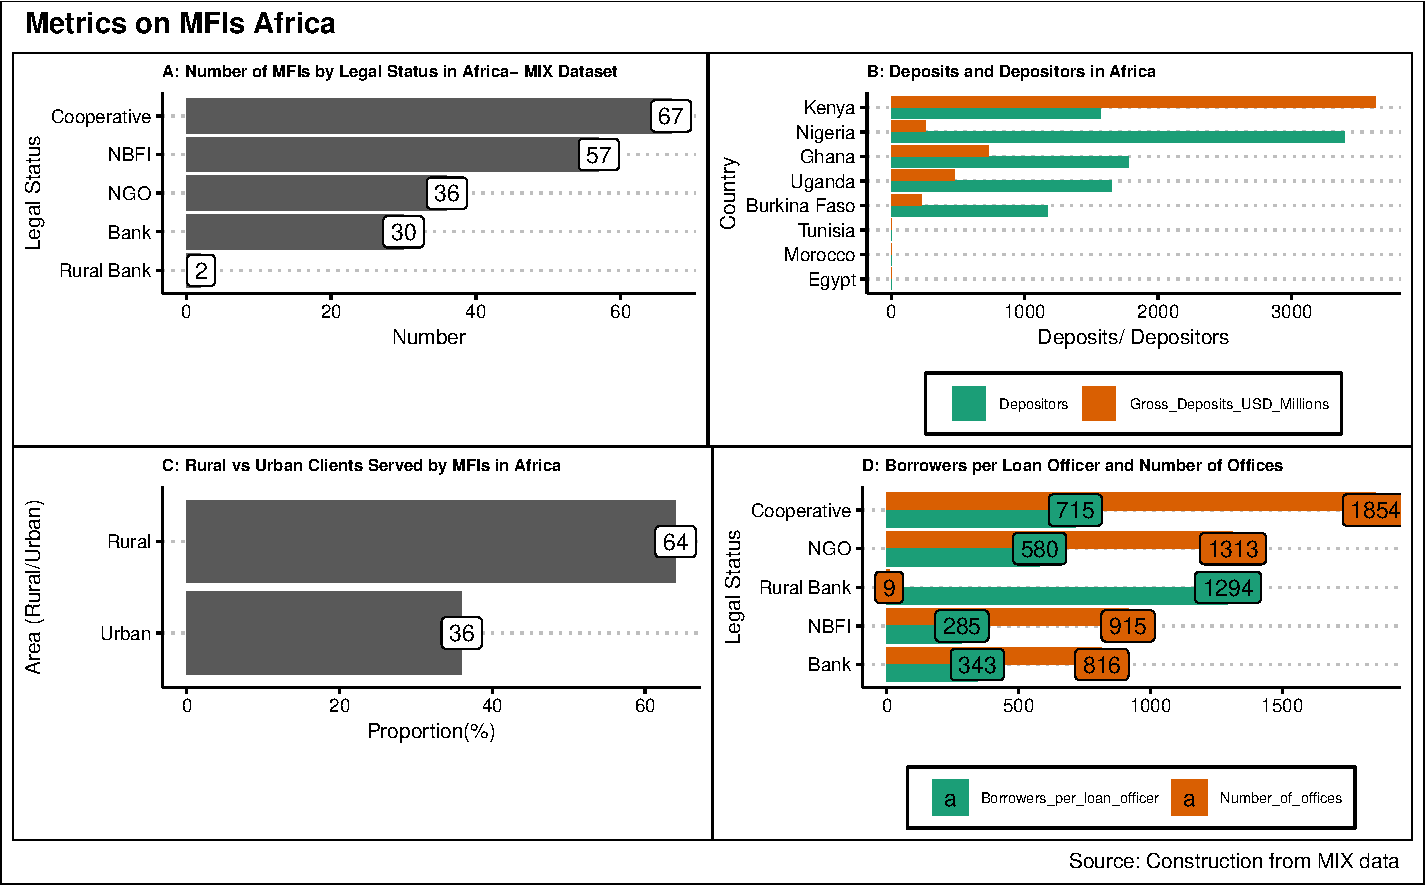
\includegraphics{_main_files/figure-latex/unnamed-chunk-8-1.pdf}
\caption{\label{fig:unnamed-chunk-8}Metrics on MFIs Africa}
\end{figure}

\newpage

\begin{figure}
\centering
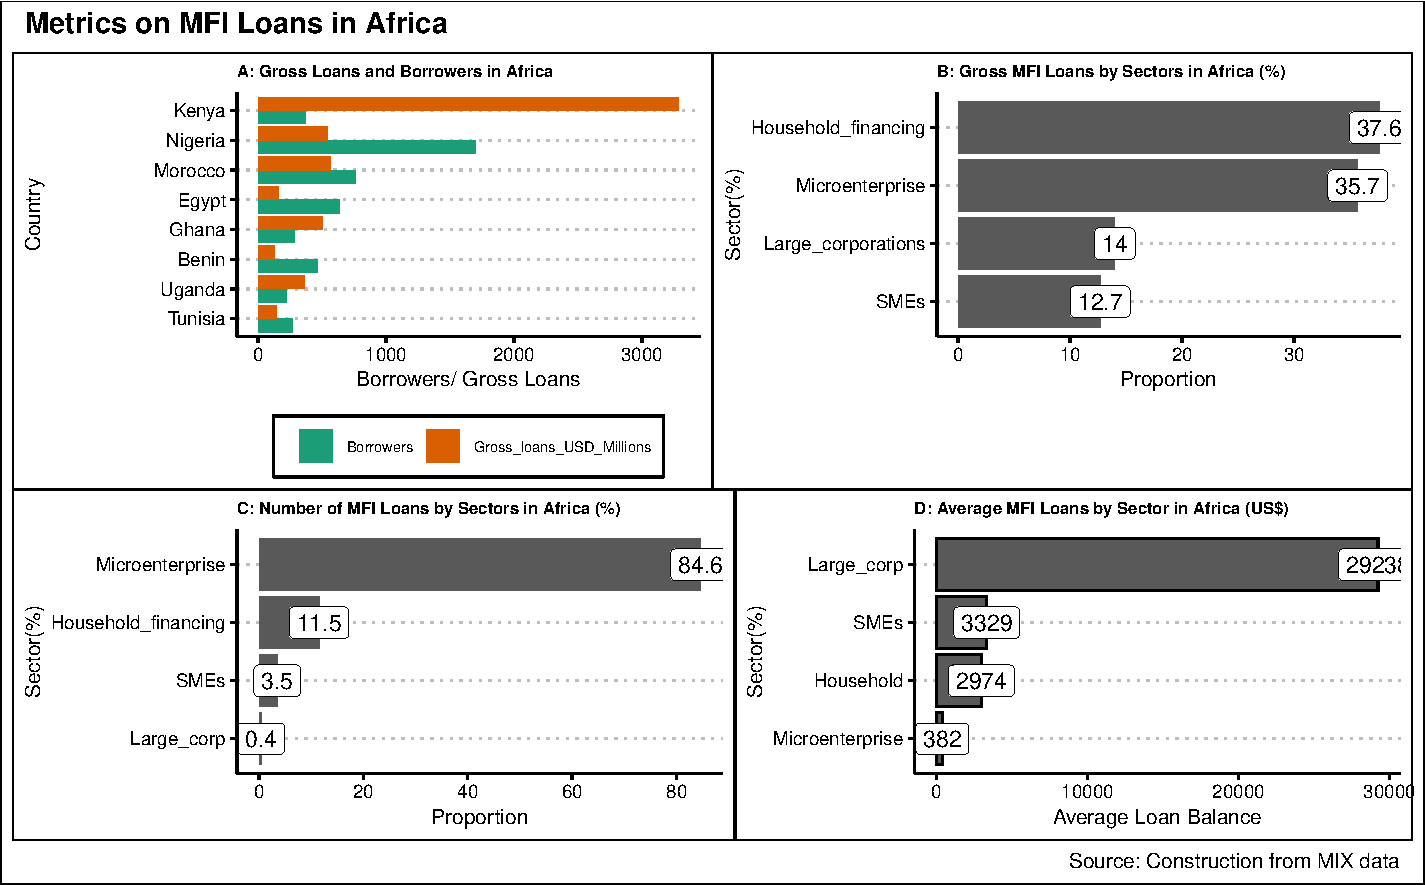
\includegraphics{_main_files/figure-latex/unnamed-chunk-9-1.pdf}
\caption{\label{fig:unnamed-chunk-9}Metrics on MFI Loans in Africa}
\end{figure}

\end{landscape}
\newpage

To illustrate the difficulty that researchers face in evaluating the impact of MFIs on the poorest segments of the society, consider the following two cases. Pitt and Khandker (1998) applied the Randomized Control Trials (RCTs) and found that group-based lending benefits the poor. However, when Roodman and Morduch (2014) replicated the study by applying a robust linear estimator and dropping outliers, they found that the results do not hold. Ghosh (2013) also replicated an evaluation report by USAID of the Self-Employed Women's Empowerment (SEWA) based in India and found most of the positive evaluations not to hold after factoring in individual characteristics of the participants. It is thus difficult to arrive at a firm conclusion that MF positively impacts on the poor given the methodological weaknesses inherent in MF impact evaluation methods (Awaworyi Churchill and Nuhu, 2016).

For the total gross loan portfolio, a similar picture emerges, although the distribution is not as extreme as that of the loan counts above. Figure 2.2 panel B illustrates that household financing and microenterprises hold the highest shares of the gross loan portfolios at 37.6\% and 35.7\%. The share of the gross loan portfolio held by large corporations and SMEs rises to 14\% and 12.7\%, respectively. Thus, although microenterprises and households produce the highest number of borrowers, the average loan amount lent to microenterprises and households is much smaller compared to SMEs and large corporations. The distribution may be an indicator or confirmation that indeed MFIs may not reach the poorest given that large enterprises receive only 0.4 \% of the loans by count but which amounts to 14\% of the gross loan portfolio.

Figure 2.2 panel D shows the average loan balances held by microenterprises, households, SMEs and large enterprises. Although large enterprises hold 0.4\% of the loans granted by count, the average loan size is 77 times larger than that of a microenterprise.
Similarly, SMEs, with 3.5\% of loans by count, have an average loan size that is nine times larger than that of a microenterprise. Thus, many microenterprises and households borrow relatively smaller amounts compared to SMEs and large enterprises. Again, it is not clear whether the loans do reach individuals at the very bottom of the pyramid where households subsist on less than a dollar a day.

\hypertarget{transformation-of-mfis-in-selected-africa-countries}{%
\subsection{Transformation of MFIs in Selected Africa Countries}\label{transformation-of-mfis-in-selected-africa-countries}}

\noindent This section highlights the extent of the transformation of MFIs in Africa. The section draws on the available data from the MIX pooled database and the IMF 2017 Financial Access Survey database. The study draws a sample of 2 countries from each of Africa's five regions based on the number of MFIs submitting data to the MIX pooled database (at least 5). Next, the relative sizes of the gross loan portfolio and deposits form the basis of the selection. However, the study also includes Ethiopia \footnote{In Eastern Africa, three (3) countries are examined. The addition of Ethiopia is based on the fact that it is among the African countries with the lowest level of capital market development, and notably lacking a stock market THE OFFICIAL MONETARY AND FINANCIAL INSTITUTIONS FORUM 2017. Barclays Africa Group Financial Markets Index 2017. Johannesburg: Barclays Africa Group Limited.. However, Ethiopia also has an extensive MF sector with substantial state involvement AYELE, G. T. 2015. Microfinance Institutions in Ethiopia, Kenya and Uganda: Loan Outreach to the Poor and the Quest for Financial Viability. African Development Review, 27, 117-129.. It is the view of the researcher that Ethiopia would be a useful addition to the study} in the Eastern African region. Table 2.3 shows the summary statistics relating to MFIs in the selected countries. Note that for Southern Africa, only South Africa meets the criteria. Botswana, Namibia, Lesotho, and Swaziland have no MFIs submitting data to the MIX pooled database.

\newpage
\begin{landscape}

\begin{table}

\caption{\label{tab:unnamed-chunk-10}Regional Statistics for MFIs, Gross Loan Portfolio, and Deposits (2015)}
\centering
\fontsize{8}{10}\selectfont
\begin{tabular}[t]{llrrrrrr}
\toprule
Country & Region & FSP.Count & Loan.Officers & No.of.Borrowers..000 & Gross\_Loans\_USD\_Millions & Average\_Loan\_USD & Desposits\_USD\_Millions\\
\midrule
DRC & Central Africa & 8 & 658 & 175 & 130.4 & 547 & 66.1\\
Cameroon & Central Africa & 10 & 1068 & 189 & 344.1 & 1824 & 408.3\\
Ethiopia & Eastern Africa & 3 & 371 & 174 & 34.8 & 200 & 12.6\\
Kenya & Eastern Africa & 11 & 2402 & 374 & 3290.4 & 1232 & 3632.0\\
Uganda & Eastern Africa & 18 & 999 & 223 & 363.3 & 230 & 472.1\\
\addlinespace
Morocco & North Africa & 6 & 3398 & 764 & 566.4 & 742 & 0.0\\
Egypt & North Africa & 4 & 1687 & 640 & 157.6 & 246 & 0.0\\
South Africa & Southern Africa & 1 & 486 & 139 & 20.8 & 150 & 0.0\\
Nigeria & West Africa & 11 & 5580 & 1699 & 542.5 & 319 & 260.3\\
Ghana & West Africa & 10 & 645 & 281 & 507.8 & 1787 & 727.4\\
\bottomrule
\multicolumn{8}{l}{\rule{0pt}{1em}\textit{Source: }}\\
\multicolumn{8}{l}{\rule{0pt}{1em}Microfinance Information Exchange, MIX (2017)}\\
\multicolumn{8}{l}{\rule{0pt}{1em}\textit{Note: }}\\
\multicolumn{8}{l}{\rule{0pt}{1em}\textsuperscript{1} The Global Outreach \& Financial Performance Benchmark Report – 2015 is the chief source of the data}\\
\multicolumn{8}{l}{\rule{0pt}{1em}\textsuperscript{2} However, the MIX database on http://www.themix.org/mixmarket/countries-regions is the source of the number of FSPs.}\\
\multicolumn{8}{l}{\rule{0pt}{1em}\textsuperscript{3} The study uses the African Union classification system on regions of Africa}\\
\end{tabular}
\end{table}

\end{landscape}

\hypertarget{manifestation-of-the-transformation-of-mfis}{%
\section{Manifestation of the Transformation of MFIs}\label{manifestation-of-the-transformation-of-mfis}}

\noindent The transformation of MFIs from NGOs to commercial entities has manifested itself in several ways. These include increased reliance on commercial capital, the advent of regulation, and a broader range of financial services on offer. The next sections describe these manifestations.

\hypertarget{reliance-on-commercial-sources-of-capital}{%
\subsection{Reliance on Commercial Sources of Capital}\label{reliance-on-commercial-sources-of-capital}}

\noindent As already noted, MFIs relied on grants and subsidies to finance their operations. However, starting in the 1990s when MFIs began to convert to formal organisations they began sourcing capital from commercial sources. However, the presence of commercial capital means that MFIs had to also strive for financial returns, given that research indicates that commercial logic drives the private funders.

Commercial capital is accessible to transformed MFIs since they appear more creditworthy. The perception of creditworthiness is especially crucial given that most investors favour the governance, risk management and regulatory oversight associated with transformed MFIs when assessing the risk-return profile of investments (Frank et al., 2008). Consequently, most of the transformed MFIs issued financial assets (debt and equity) and mobilised deposits to raise additional capital. Some MFIs are even securitising their loan portfolios, for example, ICICI (India) in 2003, the first MFI to do so (Dieckmann et al., 2007). A few MFIs have even floated their shares through IPOs, such as SKS in India in 2010 (Chen et al., 2010) and the Mexican MFI Banco Compartamos in 2007 (Ashta and Hudon, 2012). However, some researchers have disparaged the IPOs as a mechanism of self-enrichment by a few at the expense of the poor (Ghosh, 2013).

The transformation was a vital step in accessing commercial capital given that, for example, most jurisdictions do not allow non-regulated entities to collect deposits or sell financial assets (Dieckmann et al., 2007). Availability of commercial capital allowed MFIs to free themselves from capital constraints by allowing MFIs to diversify the sources of capital beyond donor funds. Also, research shows that MFIs which mobilise savings are less vulnerable to adverse market conditions (Frank et al., 2008). Likewise, donor funds are negatively prone to economic downturns and politics (Garmaise and Natividad, 2013). However, the presence of commercial capital implies that the MFIs must generate enough revenue to not only meet their social goals but to guarantee the expected financial return to the providers of capital. The presence of a financial objective and the social mission means that MFIs must optimise a double bottom line (Mersland and Strøm, 2010). MFIs must also manage their cost of capital, and deal with the agency costs arising from the entry of shareholders and bondholders.

Nevertheless, the shift to commercial model is no guarantee that funding from the capital markets will necessarily flow to transformed MFIs, Factors such as a country's legal tradition, creditor rights, and financial sector development are important determinants of the flow of formal external financing to MFIs (Tchakoute-Tchuigoua, 2014). On the other hand, the entry of commercial funding could shift the focus of MFIs away from their social mandate (Casselman and Sama, 2013). Much of the debate on transformation revolves around the effects that this shift has had on the social and financial performance of MFIs.

Bogan (2012) notes that the source of capital could influence sustainability and social mission attainment by MFIs. The roots of the argument are that funding source is directly linked to the level of monitoring and hence may incentivise or discourage efficiency. Other factors such as the regulatory environment influence the capacity of an MFI to attract certain classes of capital. Table 2.4 below highlights the relative merits and demerits of various sources of funding considering the agency theory.
It is vital to note that most of the transformed MFIs operate on a mix of various capital sources. The most common combination is that of debt, deposits, equity, and grants. Given the merits and demerits of each source, it is not clear how the influences associated with each source interact and shape the performance of MFIs, both socially and financially. Most researchers have adopted a dichotomy-based approach to the study of the sources. For example, some studies compare firms with mostly commercial funding vis-à-vis those with grants. In some other studies, researchers based their analysis on the source of funding, public or private.

\begin{landscape}

\begin{table}

\caption{\label{tab:unnamed-chunk-11}Funding Sources and Critique)}
\centering
\fontsize{8}{10}\selectfont
\begin{tabu} to \linewidth {>{\raggedright}X>{\raggedright}X>{\raggedright}X}
\toprule
SOURCE & BENEFITS & CHALLENGES\\
\midrule
Grants & Best for funding startups or risky ventures where alternative funds are unavailable
Donor monitoring improves social efficiency & No financial efficiency incentives\\
- & - & -\\
Quasi-equity & Low cost (Similar to concessional debt) & Accessible to or from mature institutions\\
- & - & -\\
Traditional Equity & Improved efficiency due to management oversight.
MFI taps into the formal capital market, making MFI independent of donors and debt-holders and other external funding & Accessible only by licensed/listed MFIs; Shareholders demands may cause short-term focus, resulting in inefficient practices
May result in mission drift\\
\addlinespace
- & - & -\\
Deposits & Low cost of funding and makes MFI independent of donors and debt-holders and other external funding & Accessible to licensed MFIs;  High costs of product development;  
High costs of product development\\
- & - & -\\
Concessional loans & Low cost of funding
Interest tax shield & Distort markets and reduce incentives to mobilise deposits
Potential financial distress (low)\\
- & - & -\\
\addlinespace
Commercial loans & Monitoring encourages efficiency
Interest tax shield & Potentially high financial distress costs\\
\bottomrule
\multicolumn{3}{l}{\rule{0pt}{1em}\textit{Source: }}\\
\multicolumn{3}{l}{\rule{0pt}{1em}Adapted from Bogan (2012)}\\
\end{tabu}
\end{table}

\end{landscape}

Beyond, monitoring, the regulatory environment may determine the sources of funding. Capital sources such as deposits, public debt, and equity are subject to regulatory approval and oversight. The next section examines the rise of regulation for MFIs.

\hypertarget{regulation}{%
\subsection{Regulation}\label{regulation}}

\noindent The financial markets legislation ``defines the rules, controls, and sanctions which restrict and enable the behaviour of participants in financial markets'' (Marti and Scherer, 2016). Legislation targeted at the MFI sector has risen concomitant with the transition from the NGO model to the commercial model. The regulation is meant to maintain stability in the MF sector (and the economy in case of spillovers), encourage competition, protect depositors and borrowers, and maintain the payment systems (Johnson, 2013). The laws targeted at the MF sector were in response to several negative experiences among MFIs across the globe, and also due to the pressure from MFIs and other interest groups for the development of MFI specific regulations (Campion and White, 1999).
In Bangladesh, for instance, indigent clients lost their savings due to the incompetence and fraud by some MFIs (Paprocki, 2016). In Nicaragua, the ``no pago'' movements raised concerns that MFIs could harm communities by trapping them in unsustainable debt (Bastiaensen et al., 2013). Moreover, cases of suicide by over-indebted MFI clients in India added to the ethical concern around MF practices (Roodman, 2012). Furthermore, a service such as deposit-taking and the entry of commercial funds meant that regulation to protect depositors and other stakeholders from the ownership and governance, management, portfolio, and new industry risks associated with commercially oriented MFIs (Meagher et al., 2006) was necessary. Finally, the 2007 global financial crisis served to illustrate that even the shadow banking system can generate economic shocks that can affect the entire financial system and indeed the economy (Meeks et al., 2017).

In the absence of MFI specific legislation, the initial MFIs that transformed did so under commercial banking laws (Campion and White, 1999, Siwale and Okoye, 2017). However, numerous countries have developed legislation specific to MF. Examples of countries that have MFI specific legislation include Kenya (2006), Bolivia (starting from 1958 to 2002)\footnote{There are several laws that govern MFIs in Bolivia. These include the Law on Banks and Financial Entities (1993), Central Bank of Bolivia Law (1995), Property \& Popular Credit Law (1998), Law for Normative Strengthening \& Financial Supervision (2001), and the Solidary Bond Law (2002). These laws apply to all private financial funds (FFPs), open savings and loan cooperatives (CACs), and commercial banks. CACs are also governed by the General Law for Cooperative Associations (1958) together with Supreme Decree No.~24439 (1996). FFPs are also subject to the Supreme Decree No.~24000 (1995).}, Nepal (1996, 1999, 2002), and Indonesia (1992, 2003) (Meagher et al., 2006). In most of these countries, the provisions in MF laws mostly follow a variant of the CAMELS rating model used in bank supervision or a variant of the model. The rules emphasise minimum capital and capital adequacy requirements, asset quality, management quality, earnings liquidity, and the sensitivity to market risk (Daher and Le Saout, 2013).

However, regulation is costly both socially and financially both to the MFIs and to the regulators. The costs arise mainly due to the involvement of a significant proportion of skilled labour necessary for effective regulatory compliance (Cull et al., 2011). Also, as Marti and Scherer (2016) argue most jurisdictions follow the technocratic approach to the development of financial regulation. Unlike the inclusive approach to legislation, the technocratic approach ignores the affected parties (like the MFI clients), focusing instead on experts and special interest groups. The inclusive approach favours both the means and the ends of financial regulation. Given the contested nature of poverty and financial exclusion, especially the approaches to tackle them, the researchers recommend the inclusive approach.

Finally, research has not found compelling results regarding the benefits of regulation on both the financial and social performance of MFIs. For example, Cull et al.~(2011) demonstrate that regulatory supervision leads to reduced outreach to women and other customers that are costly to reach. Similarly, Siwale and Okoye (2017) do not find evidence that regulation of MFIs helps augment the social mission of MFIs, just as Hartarska and Nadolnyak (2007) find no evidence that regulation positively influences both financial and social performance. The researchers do note, however, that regulation has restored confidence in the MFI sector and served to professionalise the provision of MF services.

\hypertarget{broader-range-of-services-offered-by-mfis}{%
\subsection{Broader Range of Services Offered by MFIs}\label{broader-range-of-services-offered-by-mfis}}

\noindent Commercialisation saw the reduction in donor funding and the push by commercial capital providers for a financial return, in addition to the pursuit of their social mission. Further, the commercialisation also led to increased competition between commercial banks and MFIs at the base of the pyramid. MFIs adapted to the increased competition and demands from the providers of capital by offering additional products tailored to meet the needs of the poor and the financially excluded (Cozarenco et al., 2016). The rollout of the new products was also meant to increase customer loyalty, attract new customers, reduce institutional risks and improve competitiveness (Frankiewicz and Churchill, 2011). Thus, the product range has expanded to include savings products, microinsurance, cash transfer services, pension accounts, leasing, grants, and a range of non-financial services\footnote{The non-financial services offered by MFIs include health education, skills training, and social awareness.}.

The microsavings product is similar to the savings products offered by mainstream commercial banks, credit unions, and building societies. The only significant distinction is the scale of the savings, with MFIs dealing mainly with small savings garnered from the needy individuals. Although the initial assumption was that the poor could not save due to their limited income, research indicates that the indigent clients demand both credit and savings products simultaneously (Afzal et al., 2015). However, the study concludes that the poor are a different lot and thus it is not enough to avail a savings product to them. MFIs must avail the right savings product along with facilitation as the standard savings product offered by commercial banks may not get the poor to save (Chandrasekhar and Anantharaman, 2015).

Money transfer, on the other hand, allows one party in a transaction to move cash to another individual or institution in a scenario where the physical exchange of cash is not possible. For example, M-Pesa is a popular mobile phone-based platform in Kenya that people use to pay utility bills, school fees, and even for government services (Maake et al., 2014). Before the advent of MF, such services usually involved the use of a money order drawn in a post office at substantial cost and inconvenience to the parties involved. The other mechanisms for cash transfer offered by MFIs include checks and bank drafts, electronic fund transfers (EFT), and services based on proprietary networks such as the Western Union and Moneygram (Ouma et al., 2017). Given that MFIs are accessible to the poor, they are in a better position to offer these services at the base of the pyramid.

Microinsurance, or insurance for the poor, is aimed at cushioning the poor against unexpected shocks. The low uptake of the conventional insurance products has led to the push for this model of risk mitigation. Unlike microcredit, microinsurance involves the poor making regular premium payments and cannot quickly be packaged as a group product as has been the case with the microcredit group schemes (Platteau et al., 2017). Also, Armendáriz and Morduch (2010) argue that insurance for the poor is risky given the prevalence in poor communities of infectious diseases and higher susceptibility to natural disasters like droughts and floods. Also, information problems, higher per unit transaction costs of insurance, and difficulties in contract enforcement in poor communities make microinsurance especially perilous and needing to be creatively designed.

Thus, in designing microinsurance products, MFIs must take cognisance of the precarious conditions in which the poor live. To encourage the poor to cover themselves against risks deterrents such as price, quality, trust, and liquidity must be addressed (Platteau et al., 2017, Eling et al., 2014). Table 2.6 illustrates the extremely low uptake of microinsurance in the three regions, with health insurance faring slightly better than agricultural insurance.

\begin{table}

\caption{\label{tab:unnamed-chunk-12}Uptake of Microinsurance}
\centering
\fontsize{8}{10}\selectfont
\begin{tabular}[t]{lll}
\toprule
Region & Agricultural\_Risks(\%) & Health\_Risks(\%)\\
\midrule
Africa & 0.10 & 0.74\\
Latin America & 0.36 & 1.24\\
Asia and Oceania & 0.60 & 0.74\\
\bottomrule
\multicolumn{3}{l}{\rule{0pt}{1em}\textit{Source: }}\\
\multicolumn{3}{l}{\rule{0pt}{1em}Platteau et al. (2017)}\\
\end{tabular}
\end{table}

Another product offered by MFIs is micro-pensions. Any pension scheme aims to provide some steady flow of income from retirement to death. Micro-pensions involve the medium and long-term savings schemes that generate capital which the scheme then invests in a variety of assets. The financial flows from these investments are then used to support the non-working elderly (Frankiewicz and Churchill, 2011). Pensions were devised in the western world during the industrial revolution when formal employment gradually replaced casual and self-employment. The challenge with micro-pensions is that most of the MFI clients are engaged in informal, mostly self-employment. It means, therefore that their cash flow is very uneven. Furthermore, most of the cash that the microentrepreneurs produce is prioritised towards the provision of the bare necessities of life, and not business growth or savings. Lastly, some MFIs are even involved in the distribution and marketing of clients output (Armendáriz and Morduch, 2010).

Although product diversification is beneficial to MFIs, it also poses several challenges. For example, some products may result in financial losses due to low demand or the lack of appropriate delivery channels, as in the case of micro-insurance (Platteau et al., 2017). Also, some products offered by MFIs may affect the uptake of another product, a form of cannibalisation (Elabed and Carter, 2015). Cannibalisation is frequent among the various classes of savings accounts, as the experience by Association for Social Advancement (ASA) in Bangladesh demonstrated (Campion and White, 1999, Meagher et al., 2006). Moreover, the failure of a product is likely to affect the image of the MFI among its clients. Furthermore, the diversity of products may affect the service quality as the staff's attention is spread across more products. Lastly, the primary concern in MFIs is that the product diversification may cause mission drift (Christen and Cook, 2001, Chahine and Tannir, 2010).

\hypertarget{efficiency-financial-performance-and-sustainability}{%
\subsection{Efficiency, Financial Performance, and Sustainability}\label{efficiency-financial-performance-and-sustainability}}

\noindent The entry of shareholders and bondholders in addition to the traditional donors presumably increases the level of monitoring of the management (Stoughton and Zechner, 1998). From the agency theory perspective, monitoring is one of the means of resolving the agency conflicts. Also, bondholders and shareholders are likely to give MFIs an increased commercial orientation, through, for example, the expertise they bring in by way of the board of directors and the management team they hire (Lauer, 2008).
Furthermore, some MFIs have adopted performance-based compensation schemes to address agency conflicts (Bateman, 2010a). Thus, any examination of the transformation of MFIs from lenses of the agency theory points towards improved efficiency and financial performance. Indeed, most studies have found a positive correlation between the injection of commercial capital and the financial performance of MFIs (Louis et al., 2013). For instance, Daher and Le Saout (2013) find that transformed MFIs perform better financially. They note, however, that the better financial performance is inconsistent with social performance.
Moreover, researchers have reservations regarding the improvements in financial performance by transformed MFIs. They point to the tendency of transformed MFIs to increase interest rates, engage in aggressive marketing and loan collection methods and offer incentives to managers based on volumes of loans (Ghosh, 2013). These tendencies may be detrimental to clients, lower portfolio quality, and leads to market saturation (Hoque et al., 2011).

On the other hand, there exists conflicting evidence on the effects of the transformation on social performance (and social efficiency), although increased commercial orientation may point to reduced social emphasis (Cobb et al., 2016, Daher and Le Saout, 2013). Other researchers find mixed outcomes (Abdulai and Tewari, 2017). It is then not clear whether the benefits of the transformation of MFIs accrue only to the providers of capital, clients, or to both parties. The inconsistent research output point to a significant research gap. Awaworyi Churchill and Nuhu (2016) pose an essential question, ``What has failed? Microfinance or evaluation methods?''. The lack of consensus amongst researchers despite the abundance of research in the area indicates the need for more research.

\hypertarget{enhanced-control-and-governance}{%
\subsection{Enhanced Control and Governance}\label{enhanced-control-and-governance}}

\noindent The entry of commercially oriented shareholders and debt holders has the potential to enhance the control and governance of MFIs. First, commercial funders emphasise tightening the systems of internal controls and thus leading to improved management of the MFIs (Mersland and Strøm, 2010, Mersland and Strøm, 2009). Secondly, board representatives of commercial providers of capital are likely to uphold higher professional standards and possess the technical expertise to drive the organisation in the right direction.
Also, the transformed MFI must conform with the local banking regulation, including the setting up of a board committee, management structures, disclosures, and stringent risk management procedures (Frank et al., 2008). Likewise, the transformation also leads to the hiring of experienced human resource personnel that may have a bearing on the performance of the transformed MFI. Some of the research that uncovers a positive association between MFI transformation and improved financial performance attribute part of this improvement to enhanced control and governance. However, some research finds that the governance of MFIs affects neither their financial performance nor the outreach to the poor (Mersland and Strøm, 2009).

2.10.6 Improved Customer Service
\noindent An essential consequence of the commercialisation of MFIs is customer orientation. One example of customer positioning is the development and provision of additional products like micro-insurance and microsavings (Chandrasekhar and Anantharaman, 2015). The new products are geared to meet the customer needs better. To increase customer convenience, most MFIs have adopted technology (Ouma et al., 2017). The fact that MFIs have done away with the one size fits all approach in product design is an illustration of increased customer focus.

Importantly though is that the microfinance space has become more competitive with the entry of commercial banks that offer similar products (Kar, 2016). Also, the presence of shareholders and debtholders keen on a financial return means that the MFIs must strive towards retaining the existing customers and winning over new customers (Ballwieser et al., 2012). It means therefore that the customer experience is a critical differentiator in both the financial and social success of MFIs. Thus, the transformation of MFIs usually involves significant costs in the training of staff in customer care.

\noindent Other Motives for the Transformation of MFIs
According to Christen and Cook (2001), there are several other reasons why MFIs transform into commercial entities. CGAP notes that legislative change may force an MFI to transform. For example, in Ghana, all MFIs are required to register with the Bank of Ghana (Bank of Ghana, 2016). Georgia enacted a law requiring NGOs to cease engaging in MF. Such a legislative requirement provides new institutional requirements for engaging in MF activities. MFIs also transform to gain legitimacy in the eyes of investors, customers, peer financial institutions and other lenders. The legitimacy would allow the transformed MFIs to access funds and raise additional capital with ease. Lastly, some MFIs have explicitly transformed to allow their employees or clients to become owners (Lauer, 2008). The move is designed to increase employee loyalty and minimise agency conflicts between employees and the management.

\hypertarget{challenges-of-transforming-mfis}{%
\section{Challenges of Transforming MFIs}\label{challenges-of-transforming-mfis}}

\noindent The transformation of MFIs from NGOs to commercial entities poses several challenges. First, the transformation is costly- both financially and the in the time consumed (Frank et al., 2008). For instance, transformed MFIs incur higher costs arising from the increased reporting requirements and compliance with regulatory procedures (Meagher et al., 2006). The transformation also leads to increased spending on infrastructure (e.g., physical and logical security infrastructure) and human resources (e.g., lawyers, financial consultants, managers, and MFI personnel). Finally, the new products launched by transformed MFIs require extensive market research and marketing (Campion and White, 1999).

Also, legal and other administrative challenges plague the transformation process. In Kosovo, for example, there was a ruling that declared the transformation of MFIs into shareholder-owned funds unconstitutional (The Constitutional Court of the Republic of Kosovo, 2013). On the other hand, Georgia banned NGOs from offering MF services (Lauer, 2008). In the case of Georgia, the ban meant that the NGOs had to transform, spin-off their MF segments into separate business entities or abandon the MF business altogether.
The administrative challenges arise out of three problems inherent in the conversion of MFIs into commercial stand-alone legal entities: integration into the formal financial system, ownership, and governance, and organisational development (Campion and White, 1999, Lauer, 2008, Mori and Mersland, 2014). The integration of the transformed MFIs into the financial system raises several challenges. First, in most jurisdictions, there were no specific regulations tailored for MFIs. Thus, MFIs transforming had little choice of an appropriate organisational structure (Campion and White, 1999). Most MFIs that transformed had to adopt the commercial banking structure with the attendant regulatory requirements, including the minimum capital. However, with the maturity of the regulatory framework, MFIs can choose from a variety of organisational forms, such as commercial MFIs, rural banks, commercial banks, or a variant of an NBFI. Several jurisdictions have created a legal framework specific to MFIs which has aided the transformation processes for MFIs.

Before transformation, and even after, the move from the NGO setting to a commercial setting is a challenging process for most MFIs. For instance, the MFI must expend resources to develop commercial, organisational culture, acquire additional human resources and organise training programs to orient the existing staff members on the new business model. The development or acquisition and implementation of a management information system (MIS) suited for modern banking are especially pressing and costly procedures (Campion and White, 1999). For most MFIs that have moved from the NGO model, the culture of the organisation employees must be altered to cater for a more commercial, and thus, a more customer-centric culture. These issues relating to organisational development results in substantial costs of training and mentorship (Campion and White, 1999).

Furthermore, the MFI transformation ushers in new equity and bondholders. The new ownership team involves international investors, employee stock ownership programs, and local private investors. The original NGO is usually part of the shareholding, although highly diluted (Périlleux et al., 2012). Most of the new owners require some form of financial return. In the case of K-Rep, identifying potential shareholders and negotiating a shareholder's plan took a substantial amount of time (Mersland, 2009, Servin et al., 2012, Campion and White, 1999).

Moreover, the new ownership structure requires that a board should be set up to oversee the running of the organisation. The board typically sets the mission and vision of the organisation and sets the investment strategy of the organisation. Setting up a useful board to steer an MFI through a transformation process is itself a challenge (Mori and Mersland, 2014). The new governance mechanism and the profit motive may create strains between the different stakeholders in the MFIs.

Also, the political-legal and social-economic environment pose a challenge to the transformation of MFIs, including the timing of the transformation. On the legal side, strict usury laws, tax legislation, and provisioning requirements may limit the financial sustainability of a transformed MFI (Meagher et al., 2006, Johnson, 2013). Like in the case of Georgia and Kosovo highlighted earlier, political-legal interventions may be the ultimate determinant for the decision to transform. As the experience with K-Rep shows, the economic environment has a bearing on the valuation of assets and the speed of license processing by regulators. For instance, the banking crisis in Kenya led to a delay in the licensing of K-Rep by about two years (Campion and White, 1999). The next chapter lays out the conceptual framework of the study.

\hypertarget{tables}{%
\chapter{Possible Impacts of the Transformation of MFIS: A Conceptual Framework}\label{tables}}

\chaptermark{Conceptual Framework on Transformation of Microfinance Institutions}

\minitoc 

\hypertarget{introduction-1}{%
\section{Introduction}\label{introduction-1}}

\noindent This section focuses on outlining a conceptual framework of the possible impacts of the transformation of MFIs globally and particularly in Africa. The chapter first addresses the low level of transformation of MFIs across the globe. Next, the section describes the theoretical basis for the link between MFI transformation and performance, followed by the techniques for measuring the financial and social performance of MFIs. Subsequently, the section provides a critical review of the empirical literature on the effects of the transformation of MFIs, and the relationship between ownership structure, organisational structure, and efficiency of the transformed MFIs, on the one hand, and their financial and social performance, on the other. The section concludes by examining the determinants of the performance of transformed MFIs.

\hypertarget{drivers-roadblocks-to-mfi-transformation}{%
\section{Drivers/ Roadblocks to MFI Transformation}\label{drivers-roadblocks-to-mfi-transformation}}

\noindent As noted by D'Espallier et al.~(2017a), although a substantial number of MFIs have adopted the commercial model, a significant number still operate as NGOs. Given the benefits that come with commercialisation, it is hard to justify the low levels of transformation among MFIs. Further, MFIs seeking to transform usually have substantial access to financial and technical support before and after transformation (Bateman, 2010b, Campion and White, 1999) from organisations like the World Bank, and USAID. If the transformation of MFIs is so desirable, what is hindering the mass transformation of MFIs to the commercial model? Put another way, what factors drive, enable or hinder the transformation of MFIs? The section highlights the challenges that MFIs face in the transformation process and draws insights from institutional theorists.

\hypertarget{financial-and-administrative-challenges}{%
\subsection{Financial and Administrative Challenges}\label{financial-and-administrative-challenges}}

\noindent The costs and administrative challenges of the transformation could partly explain why so many of the MFIs continue to operate as NGOs. As Campion and White (1999) note, an MFI should only undertake to transform when it is internally capable of bearing the costs and time involved. For instance, an MFI should transform when it can navigate the administrative pitfalls, like the process of applying for licensing and the attendant requirements. It is not clear at what point an MFI is internally capable of transforming either regarding financial resources (assets base) or length of operation or a combination of these and other factors. Campion and White further advised that MFIs should consider transformation only when it is the best strategy, and the regulatory environment is conducive. Researchers have not addressed these issues comprehensively in the existing literature to pinpoint the suitable preconditions for transformation. Alternate explanations for the failure by MFIs to transform come from the institutional theory.

\hypertarget{institutional-theory-perspective}{%
\subsection{Institutional Theory Perspective}\label{institutional-theory-perspective}}

\noindent The institutional theory gives some useful insights regarding inertia on the transformation of MFIs. The institutional theory seeks to explain the development of the structure of rules, norms, and routines in organisations. The theory examines how specific structures get accepted as the standard ways guiding social behaviour, and ultimately decline and get discarded (Scott, 2004). The theory holds that the institutional environment is more influential in the development of formal structures in organisations that market pressures (DiMaggio and Powell, 1991).

The institutional theory is not only focused on the persistence and convergence in organisations but is also concerned with change and de-institutionalisation. The institutional theory aims to explain the creation, transformation\footnote{In the case of MFIs, the transformation involves the deinstitutionalization of the NGO model and the institutionalization and legitimation of the commercial model of conducting MF business.} and the impacts of institutions (DiMaggio and Powell, 1991). Thus, although economic pressures have a bearing on organisations, the institutional environment significantly influences the way that actors interpret the meaning and consequences of the economic forces. Finally, the institutional theory notes that organisations often adopt established institutional structures without critical scrutiny on the path to gaining legitimacy in the institutional environment (Dacin et al., 2002).

The institutional theory draws from a variety of disciplines. In the 19th century, the theory borrowed heavily from economics, political science, and sociology. The works of Karl Marx, Emile Durkheim, Marx Weber, Herbert Spencer and Charles Cooley were particularly influential. Later, the theory expanded and borrowed from cognitive psychology, evolutionary and transaction cost economics, social history, ethnomethodology, and the new cultural studies in anthropology and sociology. Economists such as John Commons and Thorstein Veblen had argued for the examination of the historically changing rules that govern economic transactions. They pointed out that economics had overemphasised rationality and ignored habit, routines, procedures, conventions, roles, and rules as drivers of economic behaviour (Scott, 2004). Moreover, historical institutionalism stresses the role which current institutional structures play to influence subsequent arrangements and directions of change. Accordingly, historical institutionalists view the evolution of institutional structures as path dependent (Dacin et al., 2002).

As detailed by Ritzer (2005), institutional theory rests on a set of assumptions. The first assumption is that institutions, as governance structures, embody rules for social conduct. Secondly, actors accord legitimacy to those groups and organisations that conform to these rules. This legitimation is a condition that contributes to the survival of firms. In the case of MFIs, offering financial services to the poor and the financially excluded is the source of legitimacy which some researchers argue is under threat due to the transformation. Moreover, the theory assumes that inertia, a tendency to resist change, is inherent in institutions. Lastly, the historical evolution of institutions matters. The emphasis on the historical setting implies that past institutional structures constrain and channel new arrangements and shapes future evolution of firms.

One form of pressure from the institutional environment is coercive pressure. Coercion implies some form of implicit or explicit push to conform. Coercive pressure is exceptionally high where the institution is highly dependent on the institutional environment from which the pressure to conform arises (Meyer and Rowan, 1977). Pioneer MFIs were relatively more donor-dependent. Hence, donors like the World Bank and other donor agencies, had leverage to place considerable pressure on MFIs to transform especially with the rise of neo-liberalism (Ostry et al., 2017). In the case of the institutional transformation of MFIs, the donors theorised against the existing, not-for-profit organisational model. The theorisation included the specification of the failings of the not-for-profit model and the vindication of the practices of the commercial approach in light of pragmatic considerations (Dacin et al., 2002) and real or perceived benefits.

The institutional theory not only provides insights regarding the transformation of MFIs but also insights into the financial and social performance of MFIs post-transformation. Thornton (2002) provides an analogy of publishing firms that transformed from the professional editorial setup to the market-led positioning, a trend prevalent in numerous industries (Thornton et al., 2015). The author argues as follows, in line with the institutional theory:

\begin{quote}
In the context of the publishing industry, the meaning and legitimacy of various sources of organisational identity and strategy and structure are shaped by a prevailing institutional logic. Publishers may identify with publishing as a profession by building their personal reputations in the industry, or publishers may identify with publishing as a business by improving the market positions of their firms. Second, institutional logics determine which issues and problems are salient and the focus of management's attention. For example, publishers may focus on increasing sales by concentrating on author-editor networks in product development; or publishers may focus on increasing profits by emphasising control of resource competition in the product-market. Third, institutional logics determine which answers and solutions are the focus of management's attention. For example, publishers may adopt strategies of growth by focusing on organic growth and building personal imprints; or publishers may concentrate on acquisition growth and building market channels (Thornton, 2002).
\end{quote}

The dilemmas that publishers faced is similar to what MFIs are facing currently. In the context of transformed MFIs, the manifestation of social conduct is the ability to meet their social mission by focusing on the financially excluded. On the other hand, MFIs are expected to meet a new threshold of financial sustainability. The research debates points to the rationalisation of the new MFI business model. However, failure to conform to the expectations of attaining their social mission may render the new business model and even the entire MF industry illegitimate. The lack of legitimacy may put the survival of the transformed MFIs at risk.

Although the transformation of some MFIs fits well within the explanations of the institutional theory, it fails to account for many MFIs that have not transformed. The critics of the institutional theory, however, provide some useful insights into the persistence of non-transformation of MFIs. The critics contend that the theory is used merely to explain the homogeneity and persistence of phenomena and that it does not explain ``de-institutionalisation'' equally well. They argue that organisations do not merely drive change, but that they also change over time, often in response to external demands or pressure. Furthermore, the rate and nature of change differ across organisations (Dacin et al., 2002).

Contemporary research lumps together all MFIs and attempts to describe aggregate changes. However, given the specificity of the drivers to transform, such studies do not give a proper account of the reasons for transformation or the lack of it. Similarly, analysis based on global level data may crowd out institutional specific and regional specific manifestations of the institutional transformation of MFIs. It would be worthwhile to perform an in-depth study of individual organisations to uncover individual peculiarities because of the changes at the micro level, which could also include institutional specific, country-specific and regional specific drivers for MFI transformation (mersland, 2017).

Little empirical research has explored the factors that drive the decision by MFIs to transform. Most of the researchers take transformation for granted, or maybe as an occurrence that unfolds as the MFI matures. It would be worthwhile to establish the institutional and other factors that hinder the transformation of MFIs to commercial entities. Such research could point out the characteristics of MFIs that have undergone a successful transformation. Also, the research would link the pre-transformation state of the MFIs and the post-transformation financial and social performance. The output from such specifically oriented research would then point to the indicators that the management of MFIs and policymakers would consider when evaluating the success or failure of a potential MFI transformation.

\hypertarget{mfi-transformation-and-performance-theoretical-insights}{%
\section{MFI Transformation and Performance: Theoretical Insights}\label{mfi-transformation-and-performance-theoretical-insights}}

\noindent Researchers have widely explored the theme of the transformation of MFIs. The primary literature, for example, Campion and White (1999) and Mersland and Strøm (2010) mainly dealt with the implications of the transformation of MFIs, especially regarding possible mission drift. Other studies have compared commercial MFIs against those MFIs operating as NGOs. Some researchers have welcomed the presence of NGOs in the MF industry as an attempt to address market failures. However, some scholars have attacked the comparison between NGO and commercial MFIs. Central to their argument is that utility maximisation, not profit maximisation better explains the behaviour of firms in markets with mixed preferences (Bos and Millone, 2015). This section provides a theoretical background on the link between the transformation of MFIs and their performance.

\hypertarget{agency-theory}{%
\subsection{Agency Theory}\label{agency-theory}}

\noindent This section describes the agency theory and its implication to the study.

\hypertarget{what-is-agency-theory}{%
\subsubsection{What is Agency Theory?}\label{what-is-agency-theory}}

\noindent Agency theory deals with the principal-agent relationships where one party (the principal) engages another party (the agent) to act on their behalf. The principal delegate's decision making to the latter. Both the principal and the agent are interdependent but may have different goals and attitudes towards risk (Ballwieser et al., 2012, Eisenhardt, 1989). Suffice it to note that the principal-agent relationships extend beyond that between shareholders and managers, and could include, among others, the relationship between shareholders and debtholders.

\hypertarget{historical-overview-of-the-agency-theory}{%
\subsubsection{Historical Overview of the Agency Theory}\label{historical-overview-of-the-agency-theory}}

\noindent Although hardly acknowledged, Adam Smith had mentioned the concept of agency theory arising out of the separation of ownership from management in 1776. In line with the agency theory, Smith stated the following in his renowned book, \emph{The Wealth of Nations}.

\begin{quote}
The directors of such (joint-stock) companies, however, being the managers rather of other people's money than of their own, it cannot well be expected, that they should watch over it with the same anxious vigilance with which the partners in a private copartnery frequently watch over their own. Like the stewards of a rich man, they are apt to consider attention to small matters as not for their master's honour and very easily give themselves a dispensation from having it. Negligence and profusion, therefore, must always prevail, more or Iess, in the management of the affairs of such a company- Adam Smith (Jensen and Meckling, 1976).
\end{quote}

In an agency relationship, information asymmetry makes it difficult or expensive to verify what the agent is doing. Also, the divergence in attitude towards risk between the two parties is problematic because the objectives of both the principal and the agent may differ based on their risk preferences (Sun et al., 2016). Ex-ante, agents may misrepresent their abilities, and the principal cannot verify their skills at the time of hiring or even when the agent is working (Eisenhardt, 1989). The unverifiability of competencies presents the adverse selection problem. On the other hand, the agents may, after hiring, exert too little effort in their work, and also undertake other activities that are harmful to the principal (Tirole, 2006). The ex-post manifestation of information asymmetry is the moral hazard problem.

Following Smith, Berle and Means (1932) confirmed the extent of the dispersion of ownership arising from the separation of ownership from control in industrial firms in the United States. They traced the separation to the industrial revolution, the rise of stock markets, and the advent of organised labour and trade unions (Bendickson et al., 2016). Berle and Means noted that the separation meant that the suppliers of capital essentially gave up ownership to become mere recipients of financial returns, turning private corporations into quasi-public organisations. They argued that such separation disenfranchised the owners by ceding too much power to managers. Consequently, as subsequent research indicated, the dispersed ownership would result in shareholder apathy\footnote{The apathy arises due to the free rider problem. Where ownership is dispersed, no individual stockholder will be motivated to monitor the management because the entire cost of monitoring is borne by the individual shareholder, whereas the benefits accrue to all. This gives rise to rational apathy that allows the management to run the firm at their whims.} in monitoring the management (Battaglini et al., 2016).

With the inevitable separation of shareholding and management, monitoring by institutional and individual investors holding large blocks of shares could mitigate shareholder apathy. Large investors have the capacity and incentive to monitor the management given that the benefits they derive from monitoring exceed the costs of failing to do so. However, the shareholders holding a substantial equity stake could, on the other hand, abuse their position by extracting private benefits of control (Dyck and Zingales, 2004, Doidge, 2004). Hence, there is a trade-off between the potential advantages in the concentration of ownership and the drawbacks of near-absolute dispersion. Considering their findings, Berle and Means asserted that a corporate revolution had occurred and predicted that corporations characterised by dispersed ownership would dominate economic activities. They also projected growth in the size of firms and the concentration of the economy.

\hypertarget{positivist-versus-the-principal-agent-approach-to-agency-theory}{%
\subsubsection{Positivist Versus the Principal-Agent Approach to Agency Theory}\label{positivist-versus-the-principal-agent-approach-to-agency-theory}}

James Burnham (1941) stated that managers are self-interested and opportunistic, assumptions that later became central to the agency theory (Bendickson et al., 2016). Subsequently, research on agency theory followed two strands: the positivist approach and the classic principal-agent approach. As Eisenhardt (1989) notes, the two methods share a standard unit of analysis and assumptions but differ in the application of mathematical techniques, the choice of the dependent variable, and style.

The positivist approach focused on identifying the situations where the objectives of the owners and the managers diverge and suggested mechanisms for aligning the objectives. In doing so, the positivists dwelt exclusively on the agency conflicts that arise between the owners (shareholders) and the managers. Prominent examples of positivist research include Berle and Means (1932), Jensen and Meckling (1976), Fama (1980), and Fama and Jensen (1983).

Jensen and Meckling (1976) examined ownership structure, including how equity ownership by managers could mitigate agency conflicts. Fama (1980) considered the role of capital and labour markets as information mechanisms to control the management. Fama and Jensen (1983) posited that the board of directors was an information system that could be applied to lessen opportunism by managers in large corporations. The positivist approach is the most prominent in the finance literature and forms the basis of the various standard definitions of the agency theory. The paper by Jensen and Meckling (1976) is especially significant.

In this influential paper, Jensen and Meckling (1976) noted that the separation of ownership from the day to day management of the firm gave rise to agency conflicts due to moral hazards where managers do not always act in the best interests of the shareholders. These agency conflicts manifest themselves in the form of insufficient effort, entrenchment strategies, extravagant investments, and self-dealing by the management (Tirole, 2006).

Researchers have proposed mechanisms to resolve the agency conflicts, and as a result, incur agency costs. The first is the use of incentives to design an efficient principal-agent risk bearing mechanism, for example, by the use of performance-based compensation schemes. Secondly, the principal must monitor the performance of managers- for instance through the employment of auditors. Alternatively, the managers incur bonding costs to demonstrate a commitment to the principal's goals (Bosse and Phillips, 2016).
In markets with weak investors protection regulations and an extreme dispersion in ownership, institutional investors and large individual investors holding controlling stakes are better placed to monitor managers (Goergen and Renneboog, 2003). Thus, the ownership of corporations has implications on the level of monitoring and presumably the performance of firms. Finally, other mechanisms aimed at aligning the interests of the principal with those of the agents including ceding some proportion of ownership to the managers (Ang et al., 2000), the managerial labour market and the market for corporate control (Ballwieser et al., 2012). However, it is not possible to design a scheme that will fully align the incentives of managers and shareholders. This divergence results in residual loss (Fama and Jensen, 1983).

However, agency conflicts do arise between other parties beyond owners and managers. In this respect, the classic principal-agent approach extended the application of agency theory to the other forms of agency relationships such as shareholders-debtholders, employer-employee, lawyer-client, and buyer-supplier. Logical deduction and rigorous mathematical proofs are the hallmarks of the principal-agent approach. The output from this school is a set of general theories applicable to a broad variety of principal-agent relationships. Principal-agent literature addresses the agency relationship between shareholders and bondholders.

The prominent principal-agent literature includes Demski and Feltham (1978), Eisenhardt (1985), and Eisenhardt (1988). In brief, the paradigm prescribes the optimal contract (be it outcome-based or behaviour based) between the principal and the agent under varying degrees of outcome uncertainty, risk aversion, information systems, goal conflict, task programmability, outcome measurability, and the length of the agency relationship (Eisenhardt, 1989)\footnote{EISENHARDT, K. M. 1989. Agency theory: An assessment and review. Academy of Management Review, 14, 57-74. has presented a comprehensive overview of both the positivist and the principal-agent view of the principal-agency relationship.}. Both the positivist and the principal-agent paradigms are, however, complementary. The positivist approach is a subset of the broader principal-agent approach. While the positivist approach identifies the different contract alternatives to mitigate the agency conflicts, the principal-agent approach prescribes the most efficient contractual arrangement.

\hypertarget{criticism-of-the-agency-theory}{%
\subsubsection{Criticism of the Agency Theory}\label{criticism-of-the-agency-theory}}

Nevertheless, several researchers have criticised the agency theory. Much of the criticism has been directed mainly at the more popular positivist paradigm, with little of it aimed at the principal-agent paradigm. Some researchers hail the agency theory for offering a more complex view of organisations. However, Perrow (1986) condemned the positivist agency theory for being ``trivial, dehumanising, and even dangerous'' (Eisenhardt, 1989) while others scholars view it as minimalist (Hirsch and Friedman, 1986), tautological and lacking rigour (Jensen, 1983). Perrow (1986) further asserted that the theory addressed no apparent problems and was one-sided as it ignored the potential exploitation of workers. Also, he questioned the empirical verifiability of the theory, although subsequent research did test the theory empirically (Eisenhardt, 1989). The view by Perrow is in line with Hirsch and Friedman (1986) who assert that the agency theory is excessively narrow, and focused only on the stock price.

Although empirically verifiable, agency theory fares weakly in such tests. For example, Murphy and Jensen (1990) found no conclusive link between CEO pay and stock price. Frydman and Jenter (2010) found weak evidence for incentive alignment as an explanatory agency construct for CEO pay. Tosi et al.~(2000), after reviewing US executive compensation from 1936 to 2005 also found that agency theory is inconsistent with the available evidence. The most stinging rebuke of the agency theory came after the global financial crisis that started in 2007. Research into the causes of the crisis uncovered that strong incentives are not always optimal. The sub-optimality of strong incentives is especially prominent where there are no precise measures of the agent's efforts, in situations that require multitasking, and where cooperation between agents is essential. In such circumstances, Roberts (2010) argues that weak rather than strong incentives are necessary.

Additional criticism of the agency theory arises from assumptions. For instance, by self-interest, agency theory assumes that the providers of capital are responsible, whereas, the managers are opportunists waiting for every chance to swindle. However, the same could also hold for the providers of capital. As Miller and Sardais (2011) illustrated in their case study, the providers of capital may act against the long-term interest of the firm by forcing managers into actions that only have short-term benefits, but that is harmful in the long term. On the other hand, some steward like agents may use their superior information for the long-term benefit of stakeholders. Such short-termism has been the subject of research since the global financial crisis of 2007, yet there is scant research on the drivers of the myopic management (Dallas, 2011).

Furthermore, in criticising the assumption of self-interest, Bosse and Phillips (2016) view self-interest from the context of fairness and reciprocity on the part of the CEO. They argue that in the implementation of rules to check CEO discretion, boards must act with positive reciprocity to minimise welfare reducing revenge acts from the CEO. Also, the persistence of CSR initiatives by firms may be indicative of some degree of altruism amongst investors, although the motives of CSR are subject to debate (Glegg et al., 2017) which could be present in the MFIs even after the transformation. Nevertheless, research indicates that commercial providers of funds are driven by commercial logic, while development logic drives donors (Cobb et al., 2016). The self-interest assumption implies that with commercialisation, the social dimension of microfinance is likely to be secondary to the achievement of financial objectives.

Furthermore, the assumptions that organisations are profit-seeking is in direct conflict with the operation of MFIs pre-transformation. Evidence on transformed MFIs however, indicates a shift towards profit positioning (Chahine and Tannir, 2010, D'Espallier et al., 2017a). Also, agency theory leaves no room for non-pecuniary, intrinsic motivation, which is subject to debate. Furthermore, agency theory presumes that the agent's utility is positively contingent on financial incentives, and negatively with effort. Moreover, the theory assumes that time preferences are calculated mathematically using the exponential discount function. Finally, the theory assumes that both effort and motivation increase monotonically with rewards. All these assumptions have come under criticism and led to the development of behavioural agency theory\footnote{The behavioural agency theory relaxes some of the assumptions of the mainstream agency theory. In contrast with the standard agency theory which focuses on monitoring costs and incentive alignment, the behavioural agency theory (BAT) focuses on agent performance. The BAT argues that the objectives of the shareholders are likely to be achieved if the agent is motivated to perform to the best of their ability. The theory incorporates intrinsic motivation and inequity aversion, and relaxes assumptions on risk and time discounting. A detailed presentation of the study is presented by PEPPER, A. \& GORE, J. 2015. Behavioral agency theory: New foundations for theorizing about executive compensation. Journal of Management, 41, 1045-1068.}.

The other limitations of the agency theory usually arise out of the assumptions that firms operate in a tax-free environment and that stocks are non-voting. While these assumptions allow for the development of the model, they are unrealistic. The existence of taxes may explain why firms take up debt, but this does not explain why debt structures vary across industries and companies, and over time (DeAngelo and Roll, 2015), although differentials in the magnitude of the initial capital outlay explain part of the cross-industry difference.

Finally, the theory fares poorly in explaining the governance and performance of firms that are family-owned, firms engaged in strategic entrepreneurship, and those that take part in social entrepreneurship that have a double bottom line (Bendickson et al., 2016). MFIs fall into the latter category, given that they have both a financial goal and a social mission. As Bendickson et al.~(2016) conclude, insights from network theory and the social exchange theory could when used together with the agency theory, better explain the performance of firms characterised by the double bottom line.

\hypertarget{implications-of-agency-theory-of-mfi-transformation}{%
\subsubsection{Implications of Agency Theory of MFI Transformation}\label{implications-of-agency-theory-of-mfi-transformation}}

\noindent Given the agency resolution mechanisms, the transformation of MFIs to commercial entities has several implications. First, the entry of shareholders and debt-holders can induce discipline among managers given the increased monitoring. Thus, commercialisation could influence financial performance and the efficiency of MFIs (Berger and Bonaccorsi di Patti, 2006, Khachatryan et al., 2017). On the other hand, commercialisation is also likely to affect social performance (D'Espallier et al., 2017a).

Moreover, research suggests that ownership structure influences the capital structure of firms. For example, institutional ownership is associated with higher leverage ratios (Sun et al., 2016). Research further indicates that the choice of capital structure can also mitigate agency conflicts between shareholders and managers. High leverage or low equity value reduce the agency costs of outside equity (Berger and Bonaccorsi di Patti, 2006).

Also, the nature of ownership- that is, institutional, or individual and the ownership structure may also influence the degree of monitoring and hence the financial and social performance. A high level of ownership dispersion is likely to be detrimental to monitoring, as opposed to large blocks of ownership by individual and institutional investors (Becht and Röell, 1999). As noted earlier, however, such concentrated ownership may be harmful due to the tendency to extract private benefits of control.
Debt is a tool to reduce managerial discretion for two reasons. Primarily, debt reduces the free cash flows that managers can misuse or misapply. Besides, debt holders offer an additional layer of monitoring, and hence the view of banks and other financial intermediaries that provide debt as delegated monitors (Diamond, 1996). The presence of debt raises the threat of liquidation, where managers lose their salaries, perquisites, and even reputation (Jensen and Meckling, 1976).

However, the entry of debtholders in transformed MFIs poses a new set of conflict: the agency conflicts between shareholders and debtholders. As providers of capital, both shareholders and debtholders have an interest in the performance of the firm. However, the shareholders have limited liability but remain residual claimants after settling the debt. On the other hand, the debt-holders earn a fixed income but could lose their investment if the firm fails. The concern for the debtholders is that the owners may use the borrowed money to make risky investments. The motivation for the risky investment is that if the investment succeeds, the owner keeps the residual, but if it fails, the debt-holder suffers substantial loses (Chu, 2017). As a result, the debtors also monitor the management intensely.

Given this analogy, the capital structure may moderate the balance between the achievement of social goals and financial performance, given that investors are assumed to prioritise self-interest. For debtholders who are recipients of a fixed return, the emphasis on the social mission of MFIs is likely to be a disadvantage. However, the effects of the commercialisation of microfinance are likely to be subject to several additional factors. These factors comprise but are not limited to the degree of share ownership vis-à-vis dispersion. Thus, the establishment of the influence of the changes in MFIs must take cognisance of a myriad of factors both within and without the organisation that may have a bearing on the different dimensions of performance by MFIs.

\hypertarget{capital-structure-theory}{%
\subsection{Capital Structure Theory}\label{capital-structure-theory}}

\noindent The capital structure theories attempt to explain the financing mix of a firm regarding the proportion of debt and equity in the firms' long-term funding. Modigliani and Miller (1958) developed the most prominent theory of capital structure. According to this theory, the choice of the mix of debt and equity is irrelevant; that is, it does not affect the value of the firm. Later refinements of the theory to include taxation, and the costs of financial distress concluded that considering financial frictions; financing structure does matter. This section does acknowledge both the net operating income and the net income theories of capital structure. However, the section deals primarily with the Modigliani and Miller capital structure theories which dominate the thinking around the capital structure. The section also provides a discussion of the pecking order theory.

The MM theory is the backbone of modern thinking on capital structure. Developed by Franco Modigliani and Merton Miller starting from 1958, the theory has four components, namely MM propositions I, II, III and IV. In MM 1, Modigliani and Miller viewed the value of a firm and its capital structure to be independent. Put another way, the cost of capital did not vary with changing the capital structure. Instead, the value of a firm was dependent on its expected performance and commercial risk (Myers, 2001, Chang, 2015). The proposition implied that an optimal capital structure did not exist.

MM II recognised the existence of corporate taxes. With corporate taxes, they concluded that the financing structure of a firm does matter because interest on the debt is an allowable deduction for taxation, while dividends on both common and preferred stock are not (Dempsey, 2014). The variance in value between a levered firm and an all-equity firm is the interest tax shield, that is the tax-saving because of having paid interest on the debt. The inference is that the optimal capital structure is 100\% debt, which goes against the observed practice of corporate financing.

The MM III improved on MM II by integrating personal taxation. The inclusion of personal taxation changed the objective of the firm from that of minimising the corporate tax bill to that of minimising all taxes, both corporate and personal, which both the bondholders and shareholders face. Put another way the firm should arrange its financing to maximise the after-tax (both personal tax and corporate tax) income. Under this scenario, corporate borrowing is better if the after-tax income is higher than that without taxes, otherwise, it is advisable to borrow less. This approach introduced the concept of the relative tax advantage of debt. However, it is MM IV, also called the trade-off theory, that dominates the capital structure debate.

\hypertarget{trade-off-theory}{%
\subsubsection{Trade-off Theory}\label{trade-off-theory}}

\noindent MM IV was a refinement of the MM III, recognising that although debt has its merits, it raises the probability of financial distress. Thus, managers must strike a balance between the tax benefits of debt against the reality that a firm increases the likelihood of default, the higher the debt in the capital structure (De Jong et al., 2011). For this reason, MM IV is also called the trade-off theory. The costs of financial distress may be direct, for example, the legal costs of reorganisation. Indirect costs may include the loss of customers, suppliers, employees, receivables, and the loss associated with the fire sale of assets (Ehrhardt and Brigham, 2016). The following equation summarises MM IV.

\begin{equation}
V_{l} = V_{u} + T_{s} - FDS
\end{equation}

Where

\begin{itemize}
\tightlist
\item
  \(V_l\) is the value of a levered firm.
\item
  \(V_u\) is the value of an unlevered firm, that is, a firm with no debt in its capital structure.
\item
  \(T_s\) is the present value of the tax shield, the product of the interest expense and the corporation tax rate.
\item
  \(FDC\) is the present value of financial distress costs.
\end{itemize}

The introduction of financial distress has significant implications on the capital structure of firms. With financial distress costs, firms tend to avoid too much debt. Mature, profitable firms tend to rely on internally generated funds as do corporations with little cash flows and intangible assets. Firms with tangible assets for use as collateral have high leverage as do firms with high cash flows. Also, distress costs mean that firms would favour debt that is easily reorganizable, which favours bank loans rather than debt from public capital markets. For flexibility, firms tend to deal with few banks and opt for a few classes of debt (Ehrhardt and Brigham, 2016).

The trade-off theory has two important strands. As described above, the static trade-off theory seeks to balance between the tax advantage of debt and the potential costs of financial distress. However, subsequent research later demonstrated that under certain conditions, the tax disadvantage at the individual level offset the tax advantage of debt at the corporate level (Bradley et al., 1984). The research developments led to the introduction of an array of leverage-related costs such as bankruptcy costs themselves, agency costs of debt, loss of non-debt tax shields (e.g., accelerated depreciation and investment tax credits that reduce corporate tax liability), and the presence of personal taxes on dividends.

Thus, the calibration of the optimal capital structure must involve the balance between the tax benefits of debt on the one hand, and a range of leverage-related costs on the other. The choice of optimal capital structure then turned into an empirical issue investigating the significance of the various leverage-related costs. Much of this subsequent research indicates that the choice of an optimal capital structure is industry-specific, influenced by non-debt tax shields, and financial and trade cycles (Miao, 2005). Further, the level of debt varies with industry output, plant closings, firms' entry into the industry, and even capital investments by firms (Myers, 2001).
The dynamic trade-off theory asserts that firms have a target capital structure depending on their specific characteristics. Thus, firms will issue securities that bring them closer to their target capital structures (Elsas et al., 2014). In other words, the theory asserts that mean reversion to the optimal capital structures characterises firms financing. Notable in this theory, though is that firms incur costs in adjusting their capital structures to their desired optimal levels. The speed of adjustment to the optimal structures is also subject to research, and a significant point of contention for the dynamic trade-off theory. There is, however, no evidence of a universal optimal or target capital structure in firms of industries (Elsas and Florysiak, 2015).

The starting point of the critique of the trade-off theory is the empirical soundness of the model. Whereas taxes are inevitable, bankruptcy is rare, and so it is not proper to give equal weights to the probabilities in the choice of capital structure. Under this scenario, firms should have much higher leverage than is observed in practice. Whereas the tradeoff theory explains why firms adjust their high leverage by buying back debt and not by issuing new equity, it is weak in explaining extended under-leverage by firms. The under-leverage could be cured by issuing debt and buying back shares, an adjustment process rarely observed in practice (Myers, 1984).
In explaining the leverage level of firms, the trade-off theory has a very low coefficient of determination and cannot satisfactorily explain differing leverage levels across apparently similar firms. Furthermore, the theory cannot explain the choice of leverage targets by firms. Lastly, Welch (2004) notes that stock returns explain about 40\% of debt-equity ratio, a situation that should not occur if firms repurchased debt or issued equity to counteract the effects of stock returns of the debt-equity ratios. However, more recent empirical review of capital structure decisions points to a tendency for managers to issue stock when there has been a share price run-up, in support of the tradeoff theory and managerial market timing (Elsas et al., 2014).

\hypertarget{pecking-order-theory}{%
\subsubsection{Pecking Order Theory}\label{pecking-order-theory}}

\noindent Donaldson (1961) laid the foundations for the pecking order theory, stating that ``Management strongly favoured internal equity as a source of new funds to the exclusion of external funds except for occasional unavoidable `bulges' in need for funds'' (Myers, 1984). Myers and Majluf (1984) brought the pecking order theory to the fore. The theory contends that in raising capital, corporations are also subject to floatation costs- costs associated with the issuance of financial assets. The floatation costs compound the information asymmetry faced by investors. Most corporations, therefore, issue capital in a predetermined order usually starting with the cheapest. Most firms will start by raising capital internally using their retained earnings. When retained earnings are exhausted, firms resort to short-term marketable securities. Preferred stock, debt and common stock respectively are usually the least preferable (Chirinko and Singha, 2000, Fama and French, 2002).

The assumption behind the pecking order theory is that managers have an information advantage over investors (information asymmetry). Under information asymmetry, managers will tend to issue risky securities when they are overpriced. Investors, aware of managers information advantage, interpret any issue of securities as a signal pointing the valuation of the company's securities. Investors thus discount the firms new and existing securities when new issues are announced (Fama and French, 2002). Usually, investors and by extension the capital markets react negatively to new stock issues (Myers and Majluf, 1984, Chirinko and Singha, 2000). The logic behind the adverse reaction is that if the prospects of the firm were favourable, there would be no need to dilute the ownership structure, and hence reduce the future earnings per share of the firm. On the other hand, capital markets usually react positively to the issue of debt.

A more complex modification to the pecking order theory assumes that firms are concerned with, not just current financing costs but also with future financing costs. Thus, to balance the present and future costs of financing, firms with substantial expected investments maintain leverage. The low leverage helps firms to avoid having to forego future lucrative investments and minimise any material costs of financial distress. It also allows firms to avoid financing such future lucrative investments with new risky securities.
The leverage allowance is called the reserve borrowing capacity. The reserve borrowing capacity allows corporations to have the flexibility to issue securities to take up attractive investment opportunities that arise by quickly issuing debt (Ehrhardt and Brigham, 2016). Furthermore, firms tend to set dividend policies that allow the firm to meet most of its immediate financing needs using internally generated funds. In this respect, the dividend ratio maintained by firms tends to be sticky; that is, it tends to be steady, and not exhibit sudden fluctuations unless the firm is in financial distress.

Although some of the pecking order theory's predictions are valid, there is no evidence that the theory is of first-order importance in determining the capital structure of firms. For example, there is a definite relationship between expected investment and book leverage. Profitability, on the other hand, is negatively related to leverage. However, Myers (1984) cites some firms that issue stock when they could instead issue debt. Thus, the pecking order theory does not explain everything in corporate financing.
Moreover, it is hard to define the reserve borrowing capacity as this will vary from one firm to the other. Finally, the pecking order theory depends on sticky dividends but gives no hint why dividends should be sticky.

\hypertarget{factors-influencing-the-choice-of-financing-sources-by-firms}{%
\subsubsection{Factors Influencing the Choice of Financing Sources by Firms}\label{factors-influencing-the-choice-of-financing-sources-by-firms}}

The capital structures adopted by firms tend to vary across countries of operation, asset structures and operational risks faced by firms. Given that firms operate in different macroeconomic and microeconomic environments, and have different growth options, competitiveness, legal, and tax frameworks, they must adapt their capital structures to remain competitive. Thus capital structures vary across industries, countries and firm sizes. Table 3.1 and Table 3.2 summarises the firm-specific and country-specific determinants of capital structure respectively. Other than Moyo (2013) which was the primary source of information, the table lists other pertinent literature sources.

\newpage
\begin{landscape}

\begingroup\fontsize{8}{10}\selectfont

\begin{longtabu} to \linewidth {>{\raggedright}X>{\raggedright}X}
\caption{\label{tab:unnamed-chunk-13}Firm-Level Capital Structure Determinants}\\
\toprule
FIRM.SPECIFIC.FACTOR & EXPLANATION\\
\midrule
\endfirsthead
\caption[]{\label{tab:unnamed-chunk-13}Firm-Level Capital Structure Determinants \textit{(continued)}}\\
\toprule
FIRM.SPECIFIC.FACTOR & EXPLANATION\\
\midrule
\endhead

\endfoot
\bottomrule
\multicolumn{2}{l}{\rule{0pt}{1em}\textit{Source: }}\\
\multicolumn{2}{l}{\rule{0pt}{1em}Authors synthesis of literature from Moyo (2013), Gwatidzo \& Ojah, 2009, and Ojah \& Ombati (2016) among other sources}\\
\endlastfoot
Asset tangibility & Firms can use tangible assets as collateral for debt funding. Thus, firms with more tangible assets usually have more debt at a lower cost than firms with less tangible assets (Campello and Giambona , 2011;
Ojah and Ombati , 2016).\\
 & \\
Profitability, dividend and equity repurchases, and earnings volatility & Profitable firms are usually large and mature with free cash flows to support debt repayment and thus hold more debt. Firms take up debt to minimise cash that managers could misallocate. The debtholders act as delegated monitors and further act to monitor management. Similarly levered are small fast-growing firms which generate non-debt tax shields from their capital expenditures. Thus, small but fast-growing firms have higher leverage.
Firms with higher volatility have a higher probability of financial distress than those with lower volatility. Thus, firms with high earnings volatility take up less debt. (Barclay and Smith , 2005; Gwatidzo and Ojah , 2009; Ojah and Ombati, 2016).\\
 & \\
Competitiveness & Unlike firms operating in monopolistic or oligopolistic market conditions, firms in competitive industries have lower debt. The high debt would make a firm lose competitive advantage in the product market given that interest increases operating leverage (De Jong et al., 2011)\\
\addlinespace
 & \\
Size and growth rate & A large firm that has high profits, more tangible assets, and limited growth options and thus, uses debt to reduce free cash flows to curb agency conflicts. Small firms, unlike large firms, need to maintain flexibility to avoid agency costs of underinvestments. Hence, they rely more on equity (Barclay and Smith, 2005; Barclay et al., 2006; Gwatidzo and Ojah, 2009).\\
 & \\
Bankruptcy, financial distress costs and credit ratings & Firms with more debt have a higher probability of financial distress and hence borrow less. The opposite is the case for firms with less debt. Firms with higher credit ratings have higher debt, unlike firms with low credit ratings that have low debt (Barclay and Smith, 2005; De Jong et al., 2011.\\
 & \\
\addlinespace
Firm access to capital markets & The better chance the firm has access to the capital markets, the easier it can raise both debt and equity. A firm’s access to capital markets is a function of its size and financial performance . High-quality firms tend to have more leverage as they have the option to raise both debt and equity with ease. Medium quality firms are usually bank-oriented and have medium levels of debt. Low-quality firms rely on private debt which is costly or unavailable. Thus, they tend to have low leverage (Barclay and Smith, 2005; Ehrhardt and Brigham, 2016; Ojah and Ombati, 2016).\\
 & \\
Internal funds deficiency and investment programs & A firm with internal funds deficiency that has good investment options will issue more debt instruments. On the other hand, a firm with adequate internal cash and poor investment prospects tends to issue equity (De Jong et al., 2011).\\
 & \\
State of stock and bond markets, and the degree of firm capital market orientation & If the stock market is bullish, the firm will issue equity as the firm maximises net cash issue proceeds. In a bear market, managers will favour debt.  Additionally, firms will issue debt when it is cheaper and less risky than equity, and thus the cost of debt (interest rate) is a significant determinant of capital structure (Ehrhardt and Brigham, 2016).\\
\addlinespace
 & \\
Tax factors & Debt gives a tax advantage to firms, but the costs of financial distress can outweigh the tax advantage of debt. The cut-off where the tax advantage of debt outweighs the costs of financial distress is not clear-cut. However, firms will always seek to maximise the interest tax shield while guarding against the costs of financial distress. Most firms will have debt in their capital structure to take advantage of the interest tax shield (De Jong et al., 2011).\\
 & \\
Peer or industry capital structure & Financing patterns of firms tend to follow the financing structures of their peers, especially the better-performing ones. Thus, firms in an industry tend to have similar financing structures (Ehrhardt and Brigham, 2016).\\
 & \\
\addlinespace
Managerial factors & Managers strive towards earning extra material rents (perquisites). Hence, they favour higher profitability and larger firms. Managers adopt capita structures that maximise their wealth. Research indicates that inside/ managerial ownership is positively related to higher leverage. However, other researchers find the opposite and the debate is still unsettled (Agrawal and Mandelker, 1987; Kim and Sorensen, 1986; Jensen et al., 1992).\\*
\end{longtabu}
\endgroup{}

\newpage

\begin{table}

\caption{\label{tab:unnamed-chunk-14}Country-Level Capital Structure Determinants}
\centering
\fontsize{8}{10}\selectfont
\begin{tabu} to \linewidth {>{\raggedright}X>{\raggedright}X}
\toprule
FACTOR & EXPLANATION\\
\midrule
Country macroeconomic conditions and business cycles & Business cycles affect the returns on equity. The market timing theory suggests that firms will issue equity when prices are high, that is during boom periods. Conversely, firms are more likely to issue debt in bear markets Al-Zoubi et al. , 2017).\\
 & \\
The structure, performance, and regulation of the capital markets. & Countries are either stock market-oriented or bank oriented. The level of stock market development, investment banking relations, corporate governance practices and the nature of investor protection laws, determine the degree of orientation. Most firms in bank oriented countries source their capital from debt and have high leverage. Firms in stock market-oriented firms tend to issue more equity and are less leveraged (Matias and Serrasqueiro, 2017; Ojah and Ombati, 2016).\\
\bottomrule
\multicolumn{2}{l}{\rule{0pt}{1em}\textit{Source: }}\\
\multicolumn{2}{l}{\rule{0pt}{1em}Authors synthesis of literature from Moyo (2013), Gwatidzo \& Ojah, 2009, and Ojah \& Ombati (2016) among other sources}\\
\end{tabu}
\end{table}

\end{landscape}

When evaluating the factors listed above in considering the transformation of MFIs, several implications surface. First, given that access to capital markets is a crucial determinant of a firm's capital structure, the level of capital market development could play a role in the decision of MFIs to transform. Similarly, the MFI size and growth rates could also be significant predictors of the decision by MFIs to transform. The factors listed above also explain the intertemporal variations in capital structure and the speed with which firms' capital structures adjust from temporary states of disequilibria.

\hypertarget{quantifying-the-performance-of-mfis}{%
\section{Quantifying the Performance of MFIs}\label{quantifying-the-performance-of-mfis}}

\noindent Given the double bottom line characteristic of MFIs, measuring their performance is complex and contested. Extant literature measures both financial and social performance separately. Even then, researchers cannot agree on a single scale. For instance, in measuring the financial performance of MFIs and indeed of any firm, there are a variety of metrics, ranging from the return on assets, return on equity, to profit margin ratios. Similarly, for social performance, metrics range from the number of women borrowers, the average loan size to loans granted to rural dwellers.

Notable, though, is that there is no single metric used to measure both the financial and social performance of MFIs mainly because the two measures lack a standard or common unit. This section examines the variety of measures used to measure both financial and social performance of MFIs and ends by describing the recent developments in the measurement of MFI performance and offers some concluding remarks and reflections.

\hypertarget{financial-performance-of-mfis}{%
\subsection{Financial Performance of MFIs}\label{financial-performance-of-mfis}}

\noindent Firms with sound financial performance metrics can meet their obligations as they become due (Ehrhardt and Brigham, 2016). For instance, financially healthy firms can pay their employees and suppliers, and leave a surplus that they distribute to the providers of capital and/or retain some cash to expand their operations. In the case of MFIs, the better financial performance also means that they can provide MF services without excessive reliance on donations and grants. Furthermore, MFIs may apply the profits generated to expand outreach to the poor at a lower cost, a move that researchers term as cross-subsidisation and mission expansion (Mersland and Strøm, 2010). There are among several measures for quantifying the performance of MFIs, the most common are the financial ratios.
A commonly used financial ratio is the return on assets (ROA). ROA is the ratio of the MFIs net operating income and the assets.

\begin{equation}
ROA = \frac{Net Operating Income}{Assets}
\end{equation}

ROA is a simple ratio to calculate and indicates management's efficiency in utilising MFIs assets to generate returns for the providers of capital. The aim is to maximise the ratio and, at a minimum, generate enough revenue to cover the risk-free rate and compensate the providers of capital for the systematic risk facing the MFI (Mersland and Strøm, 2014). ROA lacks a clear cut off point. Researchers often use operational self-sufficiency (OSS) to measure the financial performance of MFIs. OSS is an indicator of the ability of a firm to cover its expenses. There are two variants of OSS: OSS 1 and OSS 3. OSS 1 is defined as follows,

\begin{equation}
OSS1 = \frac{Operating Revenue}{Expenses on Funding, Loan Loss Provisions, and Operations}
\end{equation}

If OSS\textgreater1, then the MFI can cover its expenses and have some leftover for growth. At OSS=1, then the MFI is just able to meet its expenses with no leftover. At the opposite end, an \(OSS < 1\) means that the MFI cannot meet its expenses (Mersland and Strøm, 2014).
OSS 2 on the other hand, is defined as follows,

\begin{equation}
OSS1 = \frac{Operating Revenue}{Operating Expense}
\end{equation}

The calculation of OSS 2 does not factor in the cost of funding. According to Mersland and Strøm (2014), eliminating funding costs is paramount given that funding sources vary a lot between MFIs and across regions. It means, therefore that managers cannot directly influence funding costs. Moreover, in the modern finance industry, operating costs are getting increasingly meaningless especially with the reduced role of physical infrastructure. The weakness of both OSS 1 and OSS 2 is that they ignore the cost of funding associated with equity (Mersland and Strøm, 2014). The omission is understandable given the difficulty in determining the cost in developing countries with shallow financial markets. Financial self-sufficiency (FSS) is another commonly used measure. FSS goes beyond the OSS 1 by adjusting the accounting values to reflect the market values in line with fair value accounting rules. With the adjustment, the FSS then becomes,

\begin{equation}
FSS = \frac{Adjusted Operated Revenue}{Adjusted Expenses on Funding, Loan Loss Provisions, and Operations}
\end{equation}

Christen et al.~(1995) developed the FSS. The researchers highlighted the need to adjust the accounting values for inflation and implicit and explicit subsidies (Mersland and Strøm, 2014). Overall, financial ratios are transparent and standardised. However, some of the figures used are generated subjectively via management judgment, for instance, provisions for loan losses (Ehrhardt and Brigham, 2016). While financial sustainability measures inform about the financial status of the MFI, they do not indicate the extent to which the MFI is reaching the poor. The next section describes the measures of the second dimension of MFI performance: outreach.

\hypertarget{social-performance-outreach-of-mfis}{%
\subsection{Social Performance (outreach) of MFIs}\label{social-performance-outreach-of-mfis}}

The other primary goal of MFIs is to supply financial products to the poor, especially women and rural dwellers, in developing countries. The extent to which MFIs can reach the poor is called outreach and is the degree of social performance. The social performance of MFIs has two dimensions: depth and breadth. The depth of outreach refers to the extent of poverty of the clients served by MFIs. The breath, on the other hand, refers to the absolute number of potential MFIs clients reached, or the scale of operations (Bibi et al., 2018).

Recognising the multi-dimensionality of MFIs, the social performance task force (SPTF) has developed several measures of social performance. Similarly, The French Comité d'Echanges, de Réflexion et d'Information sur les Systèmes d'Epargne-crédit (CERISE) also developed a set of social performance indicators (SPI) (Mersland and Strøm, 2014). The SPTF outreach composite index takes into account the ``provision of financial services to the poor and the financially excluded, improvement of quality and appropriateness of financial services, and improvement of the economic and social conditions of clients. The index also considers that MFIs must strive to ensure social responsibility to clients, employees, and the community served'' (Mersland and Strøm, 2009). Similarly, the CERISE SPI composite index makes use of ``targeting and outreach, products and services, benefits to clients, and social responsibility.'' However, given the difficulty in understanding composite indices and controversies in weights assignment when constructing indices, researchers still use the individual measures of MFI outreach (Chattopadhyay and Mitra, 2017). Researchers use several significant proxies for breadth and depth of outreach as shown in the Table 3.3.

\begin{table}

\caption{\label{tab:unnamed-chunk-15}Individual Measures of the Social performance of MFIs}
\centering
\fontsize{8}{10}\selectfont
\begin{tabular}[t]{ll}
\toprule
METRICS & PROXY\\
\midrule
Breadth of Outreach & Loan portfolio; 
Credit clients; 
Average loan; Savings; savers.\\
 & \\
Depth of Outreach & Average loan; 
Average loan/ GDP per capita; 
Female borrowers; 
Rural borrowers.\\
\bottomrule
\multicolumn{2}{l}{\rule{0pt}{1em}\textit{Source: }}\\
\multicolumn{2}{l}{\rule{0pt}{1em}Mersland and Strøm (2014)}\\
\multicolumn{2}{l}{\rule{0pt}{1em}\textit{Note: }}\\
\multicolumn{2}{l}{\rule{0pt}{1em}\textsuperscript{*} The higher the value of breadth measures, the higher the breadth of outreach.}\\
\multicolumn{2}{l}{\rule{0pt}{1em}\textsuperscript{\dag} Also, the growth of the breadth values is a vital indicator of the direction of the industry.}\\
\multicolumn{2}{l}{\rule{0pt}{1em}\textsuperscript{\ddag} For average loan and average loan divided by GDP per capita, the lower the value, the higher the depth of outreach.}\\
\multicolumn{2}{l}{\rule{0pt}{1em}\textsuperscript{\S} For female and rural borrowers, the higher the number, the higher the depth of outreach}\\
\multicolumn{2}{l}{\rule{0pt}{1em}\textsuperscript{\P} Growth rates are also significant in this respect. See Mersland and Strøm (2010) for details}\\
\end{tabular}
\end{table}

The following commentary is on a few of the metrics in Table 3.3 above. Usually, women exhibit high levels of poverty and, thus, there is an overlap between indigent clients and the number of women. Furthermore, researchers argue that a loan made to a woman may benefit the household more and, hence, the focus on women. Also, given that researchers have found high repayment rates among women, it is easier for a woman client to acquire a loan. However, as men tend to start more informal businesses, it could be that men acquire loans from MFIs through women (mostly wives). Also, credit services to women may reduce the obligation of men to contribute to their families (Mersland and Strøm, 2014).

There are two reasons why MFIs should focus on rural areas. First, income levels are lower in rural areas than in urban areas. With increased rural-urban migration, the labour force available for agriculture is reducing. Technology often fills the void left by reduced agricultural labour which calls for more investments. These technological improvements create demand for credit and other financial services (Mersland and Strøm, 2014).

Researchers have used the average loan as a proxy for depth of outreach. The lower the average loan size, the higher the implied depth of outreach (D'Espallier et al., 2017a). However, the metric has several shortcomings. First, the average loan size may increase because the financial position of the clients has increased. Also, accumulation of loan arrears may also lead to higher loan size. Moreover, even where an MFI places a cap on the loan size a client can take, the clients may respond by taking loans from multiple institutions as experience from Nicaragua and India shows (Bastiaensen et al., 2013). Further, the average loan size is affected by extreme values of some loans and also fails to consider the cross-subsidisation benefits where MFIs give massive loans to some individuals and institutions to expand outreach to the poor (Chattopadhyay and Mitra, 2017, Bibi et al., 2018). Similar shortcomings also plague the average loan size to GDP per capita metric. To address the weaknesses of both the traditional measures of the social performance of MFIs, Bibi et al.~(2018) develop a social performance metric based on market shares held by MFIs. They define their measure of the breadth of outreach as follows.

\begin{equation}
MSB_{ij} = \frac{NAB_{ij}}{TAB_j}
\end{equation}

Where \(MSB_{ij}\) represents the measure for the breadth of outreach (the market share of microfinance borrowers).
- \(NAB_ij\) refers to the number of active borrowers in MFI i in country j.
- \(TAB_j\) refers to the total number of MFI borrowers in country j.
They further define the depth of outreach as,

\begin{equation}
MSBA_{ij} = \frac{\frac{NAB_{ij}}{TAB_{j}}}{\frac{A_{ij}}{TA_j}}
\end{equation}

\begin{itemize}
\item
  Where \(MSBA_{ij}\) measures the depth of outreach. It is defined as the market share of the number of borrowers, computed as the market share of borrowers scaled by the market share of assets.
\item
  \(NAB_{ij}\) is the number of active borrowers in MFI i in country j.
\item
  \(A_{ij}\) is the total assets of MFI i in country j.
\item
  \(TA_j\) refers to the total MFI assets in country j.
\end{itemize}

Extreme values of loans influence a social performance measure such as the average loan size. The new measure of depth developed by Bibi et al.~(2018) corrects for the deficiency by using relative loan sizes in the place of absolute loan sizes. Furthermore, the value of the metrics falls between zero (0) and one (1), that strengthens comparison across MFIs. Also, the empirical tests of the suggested measures show that they provide a better measure of social performance than the traditional metrics (Bibi et al., 2018).

However, the metrics are country-specific and are not useful in the cross country, regional and global comparative contexts. Furthermore, the measures utilise a single dimension of social performance and ignore financial performance. It means that the new metrics do not present a comprehensive view of the performance of MFIs. More importantly, most researchers examine the financial performance, and the social performance of MFIs separately. A measure of the performance of MFIs that incorporates both the financial and the social metrics would be advantageous. The next section examines the recent developments in the measurement of the performance of MFIs.

\hypertarget{developments-in-assessing-performance-of-mfis}{%
\subsection{Developments in Assessing Performance of MFIs}\label{developments-in-assessing-performance-of-mfis}}

Given the shortcomings of the traditional measures of the performance of MFIs, some researchers have suggested alternate measures. Royo et al.~(2017) suggest a multidimensional measure of performance that simultaneously captures both the financial and social performance of MFIs. The measure that they have developed captures the trade-off between financial performance and social performance that has raised concerns about possible mission drift by transformed MFIs.

The measure suggested utilises the goal programming concept developed by Charnes et al., in 1955. Researchers interpret goal programming under the philosophy of satisfaction with multiple objectives, unlike the mathematical optimisation techniques that have a single objective. The central idea is that individuals desire to minimise the non-optimization of (multiple) goals. The methodology, however, recognises that it is hard to achieve all goals simultaneously.

Extending the goal programming beyond the model of Charnes, et al., the solution suggested by Royo et al.~(2017) combines different goal programming models to pick combinations of performance that have maximum consensus, and penalising combinations that have a high degree of conflict. Alternatively, the researchers could pick the combinations that have a maximum conflict against those that follow the general trend without loss of meaning. The score is the sum of all weights, which has a maximum value of one, provides the degree of the non-achievement of the set of goals, in this case, financial performance and social performance.

Another notable study by Chattopadhyay and Mitra (2017) makes a case for the adoption of a two by two (2x2) classification matrix that captures both financial and social performance. The matrix gives a code of one (1) to the MFI that meets both the financial and social objectives. The matrix codes other cases as zero (0). Table 3.4 below illustrates the classification. The researchers point out that by applying the logistic regression (LR), a variant of the generalised linear regression model, based on the matrix could shed light on the factors that affect the ability of an MFI to achieve (or fail to achieve) the twin objective of financial performance and outreach. The advantage of the proposed metric is its ability to capture both the financial and social performance in one score.

\begin{table}

\caption{\label{tab:unnamed-chunk-16}Classification Matrix: Joint Financial and Social Performance of MFIs}
\centering
\begin{tabular}[t]{llll}
\toprule
  &   & Achieves\_Financial\_Goals? & Achieves\_Financial\_Goals?\\
\midrule
 &  & YES & NO\\
Achieves\_Social\_Goals? & YES & Class 4 (SS) & Class 2 (FS)\\
Achieves\_Social\_Goals? & NO & Class 3 & Class 1 (FF)\\
\bottomrule
\multicolumn{4}{l}{\rule{0pt}{1em}\textit{Source: }}\\
\multicolumn{4}{l}{\rule{0pt}{1em}Adapted from Chattopadhyay, Manojit, and Subrata Kumar Mitra (2017)}\\
\multicolumn{4}{l}{\rule{0pt}{1em}\textit{Note}}\\
\multicolumn{4}{l}{\rule{0pt}{1em}\textsuperscript{1} In labelling the classes, we start with financial sustainability followed by social performance.}\\
\multicolumn{4}{l}{\rule{0pt}{1em}\textsuperscript{2} The letters F and S stand for Fails (F) and Succeeds (S), respectively.}\\
\multicolumn{4}{l}{\rule{0pt}{1em}\textsuperscript{3} For instance, FS means the MFI fails (F) financially but succeeds (S) socially.}\\
\end{tabular}
\end{table}

\hypertarget{mfis-transformation-and-performance-empirical-review}{%
\section{MFIs Transformation and Performance: Empirical Review}\label{mfis-transformation-and-performance-empirical-review}}

\noindent With time, a substantial number of MFIs converted to commercial entities, and empirical analysis on the effects of the transformation was then possible (Abeysekera et al., 2014, Mia and Lee, 2017, D'Espallier et al., 2017a). Some researchers hold that mission drift is bound to occur in transformed MFIs as better-off clients crowd out the poor in the access to MFI credit (Hishigsuren, 2006). Other scholars and practitioners hold the opposite view. This sections examines the arguments on either side and additional factors that may exarcerbate or reduce the extent of mission drift.

Campion and White (1999) argue that the presence or absence of mission drift in a transformed MFI is partly a corporate governance issue, and an outcome of the challenges of the scaling up of MF services. They note that good corporate governance allows the management to balance between financial performance and outreach. An alternate view is that mission drift is a misinterpretation of cross-subsidization and progressive lending. Thus, MFIs may reach out to clients who are better off to cross-subsidize loans for the poor and financially excluded (Abeysekera et al., 2014). Some research finds managers were not aware of the presence of mission drift as is quantified using the standard metrics (Hishigsuren, 2007). The finding underlines the view by Marti and Scherer (2016) that different social groups such as employees, management, and MFI clients are likely to have different views, including varying definitions of social welfare. Thus, the presence or absence of mission drift may not arise out of deliberate management decisions, but instead, out of conflicting viewpoints on social welfare between researchers, policymakers, and practitioners.

Part of the problem associated with the research on mission drift is the variety of proxies used to measure social performance. Mersland \& Strøm (2010) and many other researchers quantified social performance by the average loan balance per borrower and the ratio of average loan balance per borrower to GNI. Some researchers have reservations regarding the use of the average loan size and the average loan size scaled by GNI per capita as proxies for mission drift. The critics argue that higher average loan size could be an indicator of progressive lending and cross-subsidization. Also, a dynamic economy may benefit SMEs, which, in turn, may demand more significant loans. They also point out that regions with relatively low proportions of indigent clients might be wrongly perceived to be drifting from their mission. Also, as noted, a few large organizations and individuals have large loan balances with MFIs that may bias the average loan balance upwards without necessarily indicating the presence of mission drift. Armendáriz and Szafarz (2011) further argue that the observed higher average loan sizes by MFIs could arise from the ``interplay between their mission, the cost differentials between poor and unbanked wealthier clients, and region-specific clientele parameters'' (pp.~341).

Consequently, researchers have suggested alternate measures of mission drift including, among others, the number of women borrowers, number of loans, X-efficiency scores, yields on the gross loan portfolio, and the number of borrowers in rural areas. However, most of the studies highlighted below use the average loan size, usually scaled with the GNI per capita, as a measure of mission drift. Table () captures additional proxies for depth and breadth of outreach, their strengths and shortcomings. For lack of better metrics, researchers continue to use them.

\hypertarget{empirical-studies-demonstrating-mission-drift}{%
\subsection{Empirical Studies Demonstrating Mission Drift}\label{empirical-studies-demonstrating-mission-drift}}

\noindent Some researchers hold that financial performance and social performance by MFIs are negatively related. This view is central to the mission drift proponents who assert that the pursuit of financial goals is incompatible with the achievement of social objectives. Early empirical research in support of the hypothesis includes Christen and Cook (2001) who explored whether transformation made MFIs abandon indigent clients. They noted that transformed MFIs often had higher average loan sizes and higher average loan size scaled by GNP per capita compared to the non-transformed MFIs. Supporting this position, Kent and Dacin (2013) argue that commercial banking logic has, over time, displaced the social roles of MFIs targeted at addressing financial exclusion and poverty.

Recently, Mia and Lee (2017) also arrived at a similar conclusion by applying both static and dynamic panel data estimation techniques on a sample of 169 Bangladeshi MFIs over the period 2009-2014. The researchers conclude that mission drift may occur when MFIs seek higher financial returns. However, they note that cost efficiency neutralizes the extent of mission drift. Thus, the degree of cost efficiency is an essential moderating variable for MFIs that experience mission drift. Hence, if transformation results in an improvement in cost efficiency, then mission drift should not be a cause for concern.

Also, Cull et al.~(2011) examine the existence of mission drift in MFIs using instrumental variables regression and treatment effects to control for non-random assignment of supervision. They find that profit-oriented MFIs respond to supervision by reducing outreach to the poor and other customers that are costly to reach and instead focus on sustainability. On the contrary, MFIs running the NGO model that has a weaker commercial focus tend to maintain outreach at the expense of profitability. The researchers also find that MFIs curtail outreach to women and customers who are costly to reach. They further find that regulated MFIs with a weaker commercial focus maintain outreach at the expense of profitability. The research supports Cobb et al.~(2016) who find that private providers of funding emphasize profitability, whereas the public, donors and governments stress social performance.

Bos and Millone (2015) goes further and explores the extent of mission drift by benchmarking the X-Efficiency scores based on revenues, depth of outreach (average loan size), and breadth of outreach (number of loans). The researchers found that MFIs that have a high depth of outreach also have the highest levels of breadth of outreach and profits for the same input mix. The study further uncovers significant trade-offs between financial sustainability and social performance. Similarly, Mersland and Strøm (2010), using panel data estimations with instruments, find that high-cost MFIs, fund more individual borrowers, fewer women and focus more on urban areas. Low-cost MFIs display the reverse. These results indicate that the depth of outreach and financial sustainability could be pursued together if MFIs emphasise improving their efficiency by managing their costs.

Lastly, Dorfleitner et al.~(2017) examined the factors that cause MFIs to fail socially. First, they find that MFIs with better portfolio quality are less prone to social failure. Second, MFIs with a higher percentage of donations and regulated MFIs also have a lower possibility of social failure. Finally, they find that fast-growing MFIs are more likely to fail socially. The results indicate that financial sustainability, as proxied by portfolio quality, could play a role in the achievement of the social mission given that commercial MFIs have better portfolio quality (Tchakoute-Tchuigoua, 2010), in support of the mission expansion and cross-subsidization school of thought. Similarly, expansion of MFIs, usually resulting in a breadth of outreach, may be detrimental to the outreach to the poorest.

\hypertarget{evidence-against-the-existence-of-mission-drift}{%
\subsection{Evidence Against the Existence of Mission Drift}\label{evidence-against-the-existence-of-mission-drift}}

\noindent On the other hand, Abeysekera et al.~(2014) find no significant evidence of mission drift in their study, upon using static panel data model based on a sample of MFIs in Vietnam. For robustness, they measure outreach using a variety of measures: average loan size, interest cost to clients, and breadth of outreach. However, they uncover the presence of mission drift when they apply dynamic panel data models. The researchers conclude that the initial conditions (such as the initial average loan size, and micro-regional differences) and other time-varying factors play a role in the degree of mission drift experienced by MFIs.

Kar (2013) further invalidates the concerns about mission drift by using a sample of 409 MFIs from 71 countries. He uses a variety of proxies as well to measure mission drift, including average loan size, number of women borrowers, and the depth of outreach-profitability linkage. Using fixed effects model, and controlling for size, age, loan delivery method, legal status and geographical location, the study fails to confirm the presence of mission drift in the sampled MFIs. Thus, although mission drift could be MFI-specific, the researchers point to the lack of dynamism in age and the failure to decompose the size of MFIs into subsidised and unsubsidized components could be the significant drawbacks in establishing the presence of mission drift.

Finally, Roberts (2013) also find no evidence of mission drift. In the study involving 358 MFIs and using OLS model, he finds that although commercial MFIs reduce service to rural clients, they serve more women and maintain the same average loan size. The results imply that sustainability enables MFIs to reach more clients without necessarily locking out the poorest, a position also held by Nurmakhanova et al.~(2015) in their study based on a global dataset of MFIs.

Abdulai and Tewari (2017) uncover mixed results on mission drift. They find an insignificant link between sustainability and outreach by applying correlation analysis and the fixed-effects model. They uncover an insignificant relationship between sustainability (as measured using the operational self-sufficiency, OSS) and the average loan size scaled by the per capita GNI. However, they find the depth of outreach, measured using the number of borrowers to be positively related to sustainability. These results confirm the concerns by researchers regarding the appropriate measures of mission drift.

\hypertarget{culture-and-mission-drift}{%
\subsection{Culture and Mission Drift}\label{culture-and-mission-drift}}

\noindent Manos and Tsytrinbaum (2014) extend the research by Abdulai and Tewari (2017), exploring the place of culture in mission drift using a sample of 800 MFIs in 30 countries for the period 2000-2010. Using two-step fixed effects panel regression2, they find that MFIs that operate in cultures characterized by avoidance of high uncertainty and more future orientation perform better socially but score poorly on financial metrics. The results are in contrast with those of cultures with assertiveness and performance orientation that score better financially. Also, MFIs operating in cultures with a high score on gender equity focus less on extending financial services to the poor, as opposed to those operating in cultures with high power distance levels. Thus, cultural factors specific to countries and regions could also explain the regional variations in the degree of mission drift by MFIs.

\hypertarget{mission-drift-and-globalisation}{%
\subsection{Mission drift and Globalisation}\label{mission-drift-and-globalisation}}

\noindent Moreover, in evaluating the role of globalization on the performance and mission drift of MFIs, Forkusam (2014) find that the ratio of FDI to GDP is positively related to the average loan size, and inversely with the number of borrowers. The study applies the fixed effects panel regression to control for omitted time-invariant features such as country and culture. These relationships uncovered in the study suggest that increased globalization and the ensuing rise in international capital flows may result in MFI mission drift. The implication is that international capital in search of financial returns has little place for social performance by MFIs. It means, therefore, that international commercial capital flowing to MFIs is frought with mission drift.

\hypertarget{the-place-of-individual-credit-officers-in-mission-drift}{%
\subsection{The Place of Individual Credit Officers in Mission Drift}\label{the-place-of-individual-credit-officers-in-mission-drift}}

\noindent Interestingly, Beisland et al.~(2017) take the argument about mission drift further by arguing that the behaviour of credit officers could also explain mission drift. Their study used a mixed-methods approach. First, the researchers ran correlations and tested for differences in the mean number of clients using t-statistics and chi-square statistics. Next, they ran a pooled OLS regression and random effects regression with standard errors. To complement the quantitative methods, the researchers obtained qualitative data from focus group discussions with credit officers and managers of the MFIs.

They found a positive relationship between credit officers experience in years and the size of the loans they grant. In other words, the more experienced a credit officer is, the larger the loan size they are likely to approve. Furthermore, the researchers uncovered that credit officers with more experience approve fewer loans to the young and the disabled, in line with Labie et al.~(2015). To start with, due to the information opaqueness of MFI clients, MFIs usually give powers to credit officers to accept or reject loan applications. The subjective preferences of credit officers could then be at play in their decision making.

The preferences of credit officers could be due to several reasons. First, most MFIs have introduced incentive-based pay for credit officers and managers. The negative relationship between the compensation and risk could make credit officers shun high-risk clients (like the poor) to reduce the risk in their loan book. The results of the study are robust even after controlling for gender, education, marital status and branch affiliation. Consequently, the research recommends the training of credit officers to check the ``personal'' mission drift uncovered by the study. The results of the study suggest the need for a careful examination of the MFI-specific factors that may drive mission drift, and which researcher often miss when they use pooled global datasets.

In a similar study conducted in China, Jia et al.~(2016) examine the relationship between the personal characteristics of loan officers and the size and quality of their loans. The study applied fixed effects regression analysis at the loan officer level and assessed the period after the MFI had adopted the commercial model. The researchers found that loan officers with a career background in farming and local government were less prone to mission drift (that is, the average loan size of their portfolio did not rise), and did so without compromising portfolio quality. Thus, socially conscious MFIs could do with a human resource background check for potential recruits for loan officer positions in a bid to curb mission drift. In addition to staff training, background checks on employees, Ramus and Vaccaro (2017) also argue that stakeholder engagement and social accounting are viable ways to address mission drift among social enterprises, which includes hybrid organizations like MFIs.

\hypertarget{transformation-and-the-efficiency-mfis}{%
\section{Transformation and the Efficiency MFIs}\label{transformation-and-the-efficiency-mfis}}

\noindent The other strand of literature has examined the relationship between efficiency and the social performance of transformed MFIs. Efficiency here refers to the ratio of output to inputs by MFIs. An efficient MFI should produce the maximum possible outputs given a set of inputs. Researchers have applied several techniques to measure efficiency. However, data envelopment analysis (DEA) and stochastic frontier analysis (SFA) are the dominant techniques.

DEA is a non-parametric, a-theoretical technique that uses sets of multiple inputs and multiple outputs to estimate the best production frontier. Initially proposed by Charnes et al.~(1978), DEA involves the construction of a virtual output over a virtual input without defining a production function. There are two variants of the DEA. The original DEA-CCR (CCR for Charnes, Cooper, and Rhodes) assumes constant returns to scale. Banker et al.~(1984) developed DEA-BCC (BCC for Banker, Charnes, and Rhodes) which allows for variable returns to scale. The advantage of DEA is that it does not require the specification of the functional form for the calculation of efficiency scores Cook et al.~(2014).

Furthermore, DEA is not data demanding and can handle small samples and multiple inputs and outputs without having to standardise them. DEA also avails explicit improvement targets for inefficient decision-making units (DMUs) (Paradi et al., 2017). The downside is that DEA does not handle measurement errors well and cannot handle noise in the data, treating all deviations as inefficiencies. It also assumes that firms are homogeneous and use a similar set of inputs to produce outputs making comparisons of DEA scores more meaningful in a single country setting (Lebovics et al., 2016). Lastly, the DEA assumption that firms have control over inputs and outputs can be faulty as the environment, and the government can override the management in resource allocation.

Stochastic frontier analysis (SFA), on the other hand, is a parametric method. Aigner et al.~(1977) and Meeusen and Van den Broeck (1977) simultaneously formulated SFA. Subsequently, numerous researchers have used SFA to evaluate production, cost, revenue, profit and other models of goal attainment. The original formulation of SFA is as follows.

\begin{equation}
\beta{x} + v - u
\end{equation}

In the equation, \(Y\) is the observed outcome, and \(\beta{x} + v\) represents the optimal or stochastic frontier, for example, the maximum production or the minimum cost. In the optimal frontier, \(\beta{x}\) is the deterministic part whereas \(v\) is the stochastic part. The amount by which an entity fails to reach the stochastic frontier is the level of inefficiency that \(u\) captures. There are many extensions of SFA that are beyond the original specification. SFA allows for technical inefficiency but also provides for random shocks beyond the control of management that may affect output (Kumbhakar et al., 2015). The limitation of SFA is the assumption that there exists a functional form. Furthermore, it is hard to specify the error structure, especially the probability distribution. Lastly, the premise of continuity inherent in SFA and other econometric approaches to measuring efficiency may lead to approximation errors (Cullinane et al., 2006).

Thus, for given MFI inputs, how much is the MFI able to generate regarding financial returns and outreach to the poor. Lebovics et al.~(2016) explore whether there is a trade-off between financial efficiency and social efficiency of MFIs in Vietnam. They use DEA to quantify both financial and social efficiency. The study uses regression analysis and uncovers no trade-off between financial efficiency and social efficiency. The results do not favor either the poverty-lending view or the financial-systems view approaches to MF provision. These results are similar to those of Bedecarrats et al.~(2012) who argue that MFIs could achieve both financial and social performance as long as the MFI has practical social performance management strategy. These views reinforce the argument by Abeysekera et al.~(2014) that mission drift could be a corporate governance problem.

Haq et al.~(2010) examined the efficiency of 39 MFIs from Africa, Asia and Latin America using the DEA approach. The objective was to uncover the MFI types (Bank MFIs or NGO MFIs) that were most efficient at simultaneously minimising costs (hence maximising financial performance) and reaching out to poor households. Under the production approach, they found that NGO MFIs are the most efficient at reaching the dual objectives. However, under the intermediation approach, the research indicates the reverse. The results show that Bank MFIs could be better suited to lower costs associated with defaults. However, NGO MFIs achieve the dual objectives of financial sustainability and performance better.

Research by Hermes et al.~(2011) used a sample 1,300 observations and measured efficiency using SFA. The study found a negative relationship between outreach and efficiency of MFIs. More specifically, the study found that those MFIs with low average loan balance- a measure of the depth of outreach, are less efficient. Moreover, the study finds a negative relationship between breadth of outreach as measured using the number of women borrowers and the efficiency of MFIs. The argument presented to explain the negative relationship between efficiency and outreach is that transformation of MFIs generates costs which drive down outreach, especially to high-cost clients (Cull et al., 2011). Roberts (2013) also concludes that commercialization of MFIs moves them further away from their efficient frontier of social performance. Also, there is a direct relationship between commercialization, operational costs, and interest rates.
Similarly, Abate et al.~(2014) also use the SFA approach and find that there is a trade-off between outreach and the efficiency of MFIs in Ethiopia. The researchers first run an SFA regression and obtain the error term, µ, which is the measure of inefficiency. Next, they regress the inefficiency score against average loan size, women borrowers, and organization form, while controlling for age and size of the MFI.

Serrano-Cinca and Gutierrez-Nieto (2014) also recommend the need for cost efficiency by transformed MFIs in the face of reduced donor support. Their research draws on the Pareto 80/20 principle and logistic regressions on data for both drifted and non-drifted MFIs. The researchers draw parallels with the dot-com industry and recommend that MFIs should focus on raising their efficiency levels instead of raising prices (interest rates). Finally, they recommend a business model based on high turnover, instead of wide profit margins to drive MFI sustainability. However, given the intense competition in the MF sector, it is not clear whether the high turnover, low margin MFI business model is feasible.

\hypertarget{capital-structure-and-the-performance-of-mfis}{%
\section{Capital Structure and the Performance of MFIs}\label{capital-structure-and-the-performance-of-mfis}}

\noindent Before transformation, the presence of donations in the capital structure of MFIs was indicative of an emphasis on the social mission. It is, however, unclear whether the entry of commercial capital could overwhelm the social orientation of MFIs. From the business strategy perspectives, it is not apparent why commercially driven individuals and entities should care about the social performance of the MFIs. However, some researchers posit that corporate social responsibility (CSR) activities serve to resolve information asymmetries between firms and creditors. Hence, firms with a social mission have higher leverage and exhibit a faster speed of adjustment to the target capital structure (Yang et al., 2017).

The research output on the relationship between leverage and financial performance is mixed. Some researchers have found the relationship between leverage and financial performance to be positive. For instance, Detthamrong et al.~(2017) find such a positive relationship in their study of Thai firms using OLS regression. Also, Abor (2007) using data for SMEs from Ghana and South Africa and applying panel regressions that debt level is directly related to financial performance as measured by Tobin Q.

The other studies that also conclude that a positive relationship between capital structure and financial performance exists include Abor (2005), Berger and Bonaccorsi di Patti (2006) and Gill et al.~(2011). For instance, Fosu (2013), using fixed effects model and GMM finds that leverage is positively related to financial performance, with competition-enhancing the relationship. Most of these studies fail short of explaining the reasons behind the relationship. The study by Chakravarty and Pylypiv (2015) that finds that MFIs with private funding are better able to screen borrowers and monitor borrower repayment rates. Consequently, such MFIs have lower portfolio risk and fewer delinquent loans. The results of this study could explain the positive relationship between capital structure and financial performance of MFIs.

Other studies, mostly based on emerging markets point to a negative relationship between debt and financial performance. The results imply that the costs of financial distress outweigh the benefits from the tax shields, at least in developing countries (Le and Phan, 2017). Similarly, Zeitun and Tian (2014) also uncovered a negative relationship between leverage and both the accounting and market measures of performance of firms in Jordan. Similarly, Hamid et al.~(2015) uncover a negative relationship in their study based on family firms. These results could be indicative that for MFIs, the costs of potential financial distress exceed the benefits generated by the interest tax shields. The introduction of private capital could also make managers of MFIs risk averse and thus set aside much higher than optimal precautionary savings to deal with any potential financial distress, as do MFIs facing subsidy uncertainty (Armendáriz et al., 2013a).

Midway between the two extremes, some researchers posit that capital structure can have both positive and negative effects on a firms financial performance. Such researchers have proposed that at low levels, firms reap the benefits of the tax shield, which gets overwhelmed by the costs of financial distress beyond a limit of leverage. The study by Lin and Chang (2011) is an example of research supportive of this position. Margaritis and Psillaki (2010) also arrived at similar results by applying the quadratic functional form. From the discussion, the research on the link between capital structure and the financial performance of firms is inconclusive even in the mainstream corporate finance. The mixed results point to critical moderating variables on the link between capital structure and financial performance. The variables could relate to firm-specific factors and cross-country heterogeneity.

Nevertheless, researchers have extended the study of the link between to capital structure to financial performance to MFIs. Khachatryan et al.~(2017) find a link between the level of deposits in the previous year and financial performance using data from Eastern Europe. The positive relationship indicates that deposits could lower the cost of capital and hence increase sustainability. Further, they find that concessional loans do not significantly affect financial performance. Social loans and subsidies, however, are associated with lower profitability. However, the study does not delve into the possible impacts of equity capital and debt on the financial performance of MFIs. Filling this gap, Ayele (2015), using data for MFIs operating in Ethiopia, Kenya and Uganda found a negative relationship between debt-to-equity ratio and financial viability. Although these studies differ in countries covered, institutions considered, methodologies and data representation, the lack of a consensus makes policy-making difficult at the institutional and national levels.
In their research in the context of social performance, Khachatryan et al.~(2017) find a positive relationship between social grants and the depth and breadth of outreach using seemingly unrelated regressions. Further, they found that concessional loans are positively related to outreach, as do social loans and subsidies. Another study by Hoque et al.~(2011) found that leverage has adverse effects on outreach, productivity, and risk. They note, for example, that although the absolute numbers of indigent clients reached by MFIs increase, the proportion goes down due to the increased cost of capital, which implies higher default rates and hence higher portfolio risk.

On the contrary, Kyereboah-Coleman (2007) applied pooled OLS and the fixed effects model on a panel dataset of MFIs in Africa and found a positive relationship between leverage and financial performance. The researcher also found that leveraged MFIs enjoys economies of scale, allowing them to deal with information asymmetry and hence lower portfolio risk. Similarly, Dorfleitner et al.~(2016) examined the factors that influence access to debt capital by MFIs using probit and Poisson regressions. The study uncovered a positive relationship between MFI access to MF Investment Vehicles (MIV) funding to maturity (measured by age, size of MFI and debt-to-asset ratio) and performance. For instance, more mature MFIs easily access debt capital from MIVs, as do firms with better financial performance regarding portfolio quality. Furthermore, MFIs that retain focus on their social mission have better access to debt financing. These results indicate that mature MFIs with better financial and social performance should then have more debt in their capital structure than do firms that do not meet the criterion.

\hypertarget{subsidies-and-grants-and-the-performance-of-mfis}{%
\section{Subsidies and Grants and the Performance of MFIs}\label{subsidies-and-grants-and-the-performance-of-mfis}}

\noindent It appears that the presence of donor funds is also a significant driver of social mission achievement, either because it allows MFIs to lower their cost of capital, reduces the pressure on the management to make profits or that donors emphasize on the outreach to the poor. Overall, the researchers note that there is a thin line between mission drift and cross-subsidization, which makes it difficult for researchers to distinguish them empirically. However, when D'Espallier et al.~(2017a) use the event study methodology, which addresses the concerns highlighted above, they still uncover a sharp rise in average loan size attributable to the transformation of MFIs.

In their analysis of the effects of aid volatility on mission drift, D'Espallier et al.~(2017b) find that average loan size is inversely related to aid volatility. On the other hand, interest rates charged on loans are directly related to aid volatility. The researchers conclude that most MFIs have internalized and use average loan size as a signalling device to demonstrate a commitment to the social mission. They also use interest rates to adjust for uncertainty. Armendáriz et al.~(2013a) argue that subsidy uncertainty results in mission drift among MFIs as they seek to build up precautionary savings to cushion themselves financially by serving wealthier clients.

For MFIs, subsidies form a substantial percentage of the ownership structure of MFIs. Except for 23\%, the other MFIs have a portion of subsidies and grants in their capital structure (D'Espallier et al., 2013). Analysing the effects of capital structure on the performance of MFIs is more complicated in the presence of the subsidies and grants. Research indicates that donors direct most of their funding to those MFIs that meet their social mission. Even for the MFIs that have not transformed, there is a significant reduction in the magnitude of donor support. Consequently, these NGOs have adopted various mechanisms to run their operations in the face of the reduced financial support from donors.

D'Espallier et al.~(2013) note that in Africa and Asia, MFIs cope with the lack of donations by charging higher interest rates. In Latin America, on the other hand, MFIs with less donor funding tend to serve fewer women. Unsubsidized MFIs in Eastern Europe and central Asia serve less indigent individuals. Overall, the researchers find that the lack of subsidies worsens the social performance of MFIs, but the effects vary across regions. Also, they argue that there exist trade-offs even among the social measures, for instance between service to women versus interest rates charged (D'Espallier et al., 2013). However, researchers have not arrived at a consensus regarding the existence of mission drift for transformed MFIs.

Furthermore, Cozarenco et al.~(2016) analyze the characteristics of MFIs that supply savings products on a global dataset of 722 MFIs for the years 2005-2010. They find that MFIs that receive donations and subsidies have a lower tendency to offer savings products. They conclude that subsidies and grants generate negative externalities on product diversification by MFIs.

Some research also indicates that the source of the donations matters. For instance, Chakravarty and Pylypiv (2015) find that MFIs with more private donor funds tend to have lower rates of the portfolio at risk and fewer delinquent loans. Thus, the management of such MFIs improves significantly with private funding, presumably due to the monitoring role that private funders play. In a related study, Hudon (2010) also notes that better-managed MFIs tend to attract more donations. Overall, the presence of subsidies appears to have a significant link with the social performance of MFIs. However, the presence of subsidies may discourage the development of products, such as savings. Lastly, the source of the funding matters, with MFIs relying on public subsidies faring worse on both metrics.

\hypertarget{what-are-the-determinants-the-capital-structures-of-transformed-mfis}{%
\section{What are the Determinants the Capital Structures of Transformed MFIs?}\label{what-are-the-determinants-the-capital-structures-of-transformed-mfis}}

Research on the determinants of the capital structure of MFIs is scanty. Most of the available literature deals dwell on the capital structures of mainstream corporations. For financial institutions, which come close to MFIs, Gropp and Heider (2010) found that the determinants of capital structure for financial firms are like those of non-financial firms and that capital regulations and buffers are of secondary importance. Section () covers the determinants of the capital structure of corporations in detail.

Additionally, Ledgerwood and White (2006) attribute the capital structure of MFIs to maturity and the institutional life cycle. The institutional life cycle theory posits that the financing stricture of an MFI varies with the stage of the MFI in the life cycle. At the early stages, the MFIs finance their operations mainly through donations and concessionary funds, given that commercial funders find MFIs too risky. At the early stage, most MFIs operate as NGOs. In the second phase, MFIs tend to focus on the expansion of operations and thus look beyond donations to meet their financing needs. The MFIs supplement their donor funding and subsidies with equity financing (from NGOs and public investors) and seed capital from international finance institutions. At the final consolidation phase, MFIs concentrate on attaining sustainability and formalizing their operations. At the consolidation phase, MFIs raise additional capital through debt (using foreign donor funds as guarantees) and deposits (Bayai and Ikhide, 2016).

Rsearchers like Bayai and Ikhide (2016) attribute part of the disparities to regulatory provisions relating to the ways MFIs can raise capital as well as historical legacies on saving and lending. Thus, the level of maturity of an MFI is likely to affect the capital structure of MFIs. For individual sources of capital, research indicates that donors are likely to contribute more to MFIs that have verifiable accounting information, and those MFIs that emphasize on their social mission (Hudon, 2010).

Also, donors funding is positively correlated with the tangible assets, past due loans and the size of an MFI, indicating that even donors evaluate the riskiness of the MFIs they fund, using this information as a screening mechanism. However, donor funding is not influenced by the profitability of the MFI, meaning that indeed donors mostly have a social orientation. On the other hand, more profitable firms (with more even profit distribution) with more tangible assets (and bigger) and with a corporate organizational structure have easier access to debt capital. Moreover, the credit ratings of the MFIs do not influence their capital structure (Tchakoute-Tchuigoua, 2015).

\begin{savequote}
Change has a considerable psychological impact on the human mind. To the
fearful it is threatening because it means that things may get worse. To
the hopeful it is encouraging because things may get better. To the
confident it is inspiring because the challenge exists to make things
better.
\qauthor{--- King Whitney Jr. \autocite{Darwin1859}}\end{savequote}



\hypertarget{transformation-of-microfinance-institutions-in-africa}{%
\chapter{Transformation of Microfinance Institutions in Africa}\label{transformation-of-microfinance-institutions-in-africa}}

\minitoc 

\begin{quote}
\hypertarget{abstract}{%
\section{\texorpdfstring{\textbf{Abstract}}{Abstract}}\label{abstract}}

We examine the factors driving non-governmental organisation microfinance institutions to convert to the commercial, profit-oriented model. Using data from the World Bank and the International Monetary Fund (IMF), we ran logit, probit, and multinomial logit models with NGOs as the base outcome. At the firm level, age, size influence transformation. Legal tradition, institutional quality, and stock market development are significant factors at the country level. However, private credit to GDP and GDP growth rates are not significant drivers of conversion. Older firms are less likely to be NGOs, as are MFIs in civil law countries. Larger MFIs and MFIs located in countries with ``other'' legal traditions are more likely to be commercial. Institutional quality raises the chances of conversion, while stock market capitalisation relates negatively with transformation. Overall, the model does better than a null model, and the results remain robust to removing outliers.
\end{quote}

\hypertarget{background}{%
\section{\texorpdfstring{\textbf{Background}}{Background}}\label{background}}

The modern micro-finance (MF) industry draws its popularity from the promise of providing appropriate and affordable financial services to the population under-served by mainstream financial intermediaries \autocite{morduch1999microfinance,morduch2000microfinance}. The motivation for reaching out to the unbanked draws from researchers and development practitioners view that financial inclusion leads to welfare improvements for the recipients. As examples, some scholars associate access to finance with more business start-ups, higher savings rate, improved health, less child mortality, and higher education attainment by the poor, although other scholars downplay these findings \autocite{klapper2015role,o2017systematic,shahriar2017lender}. Much of the initial efforts to provide financial services to the unbanked rested on Microfinance. Microfinance refers to either the practice of delivering appropriate and affordable financial facilities to the financially excluded or the providers of such services \autocite{ledgerwood2006transforming}.

Pioneer Microfinance Institutions (MFIs), like Grameen Bank, mostly operated as Non-Governmental Organisations (NGOs) following the welfare approach, where the profitability of the institution played second to availing financial services to the poor \autocite{chahine2010social,d2017ngos}. However, the paradigm shift is towards the financial systems approach where MFIs operate under market principles, leading to charges of ``financialisation'' of poverty \autocite{mader2015financialization}, with the relatively higher interest rates charged to the clients equated to a ``poverty penalty'' \autocite{chen2017microfinance}. Some scholars and practitioners argue that MFIs following the profit-oriented financial systems model, though more financially sustainable, are subject to ``mission drift''. Mission drift refers to situations where MFIs lessens their commitment to availing financial services to the financially excluded to pursue profits \autocite{jia2016commercialization,mia2017mission}.

However, given the social mission inherent in MF, MFIs following the financial systems approach risk their legitimacy in society and local and international donor community, a significant source of funding even for commercial MFIs \autocite{nason2018behavioral}. For these reasons, some researchers and development practitioners vouch for the welfare approach, where MFIs focus primarily on the mission to reach the financially excluded without emphasizing profits. Most MFIs following the welfare approach are non-governmental organizations (NGOs). Though not subject to mission drift, the NGO model is over-reliant on volatile local and international donor funds and government subsidies \autocite{garmaise2013cheap,d2017aid}. Additionally, NGOs may crowd out the efficient, market-based microfinance providers \autocite{kota2007}, which may hurt aggregate welfare in the long run.

The win-win school attempts to reconcile the financial systems and welfare approach to microfinance. Adherents of the win-win school postulate that it is possible to achieve both financial sustainability (that is, turn a profit) and, at the same time, reach the financially excluded \autocite{kodongo2013individual}. As a case in point, some researchers argue that MFIs could strive to generate profits by offering financial services to the relatively well-off at market rates. The MFIs could then use the returns to subsidise the provision of financial services to the poor under a form of price discrimination, leading to ``mission expansion'' as opposed to mission drift \autocite{mersland2010microfinance}.

Globally, the shift from the pure welfare approach of MF provision is gaining ground. Most of the transformed MFIs operate at some point on the continuum between the NGO, welfare model and the financial systems approach \autocite{armendariz2013subsidy,d2013unsubsidized,hishigsuren2006transformation}. It all started in 1992 in Bolivia when Prodem, an NGO, converted to a commercial bank, Bancosol \autocite{fernando2004micro,creedy2018types}. Since then, many MFIs worldwide have converted from NGOs to commercial firms seeking to make profits.

This article explores the factors that drive the transformation of MFIs from NGOs to for-profit firms in Africa. To this end, we use a panel dataset of 705 MFIs in Africa from the MIX pooled database, with additional data from the World Bank- the World Development Indicators (WDI), the Worldwide Governance Index (WGI), and the Global Financial Development Databases (GFDD). We focus on Africa given the relatively low levels of financial inclusion on the continent \autocite{demirguc2018global}and the shortcomings inherent in combining data from different regions that may yield results that are not actionable. As \textcite{d2017ngos} and \textcite{wang2015ownership} suggest, the nature and performance of MFIs are country-specific. Hence, research focusing on particular regions, countries or even firms could better inform policy making.

This article contributes to the literature in two main ways. First, the study sheds light on the drivers of the transformation of microfinance institutions in Africa. Much of the literature has not examined this phenomenon, focusing on the shift's consequences and how MFIs can balance financial and social missions \autocite{d2013unsubsidized,forkusam2014does,mia2017mission}. We believe that our analysis could form a reasonable starting point for analysing the transformation of MFIs in other regions or countries. Second, we detail the linkages between the drivers of micro-finance institutions' transformation, showing how they interact to change the likelihood of conversion. We highlight the pitfalls that bedevil analysis pools data from heterogeneous sources, which may mask crucial differences or similarities between the analysis units.

The rest of the article is structured as follows. Section 2 presents the theoretical underpinnings and empirical findings related to the study. Subsequently, in section 3, we offer a summary of findings before delving into the analysis method and results in sections 4 and 5, respectively. Section 6 concludes.

\hypertarget{related-literature}{%
\section{Related Literature}\label{related-literature}}

Much of the early literature on the institutional change of MFIs dealt with the theoretical, philosophical, and historical basis for the transformation of MFIs from NGOs to commercial firms and the potential impacts of such conversion {[}\textcite{campion1999institutional}; christen2001commercialization; \textcite{gutierrez201920}; \textcite{zaby2019science}{]}. Views of scholars regarding the transformation of MFIs drew from the institutional theory on the persistence and convergence in organisations, including change and de-institutionalisation within firms \autocite{scott2004institutional} and the dominance of neoliberalism after the end of the cold war \autocite{ostry2017}.

The institutional theory holds that the institutional environment is more influential in developing formal structures in organisations than market pressures \autocite{maggio1991}. Coercion is one form of pressure from the institutional environment that makes organisations adopt institutional structures and practices. Institutional theorists note that stakeholders could force firms to adopt specific organisational structures and practices without critical scrutiny to gain legitimacy in the institutional environment \autocite{scott2004institutional,martinez2017coercive}.

With this hindsight, \textcite{bateman2010doesn} traces the pressure to convert MFIs from NGOs to the commercial model to the rise of neo-liberalism and the insistence that firms be financially self-sufficient instead of relying on government subsidies and, in the case of MFIs, donor funds. The wave of economic liberalisation and privatisation commenced in the early 1990s due to neo-liberalism \autocite{silva1998neoliberalism}. Researchers point to pressure from financiers of MF such as USAID and the World Bank as a significant driver for the decision for MFIs to transform \autocite{ostry2017}.

However, given that MFIs have a social mission, the transition to a market-led positioning is bound to conflict with the social objectives and threaten the MF industry's legitimacy \autocite{ramus2017,nason2018behavioral}. Specifically, the quest to satisfy both financial objectives and the social mission is likely to conflict, which may cause ``mission drift'' \autocite{mersland2010microfinance,mia2017mission}, where MFIs give greater priority to profitability than outreach to the unbanked.

Nonetheless, the push from donors to transform MFIs seems to contradict the slow pace of the transformation. NGOs still form a substantial proportion of MFIs in Africa, accounting for 32\%, second only to Non-Bank Financial Institutions (NBFIs) at 40\% \autocite{market2018global}. A question arises regarding the factors behind the persistence of certain organisational forms of MFI provision in Africa and across the globe. \textcite{pashkova2016business} tackled this question. They found that the cooperative model is prevalent in economies with civil law systems, low inflation levels, and high economic growth rates.

In contrast, NGO type MFIs feature in countries with high inflation rates and low economic growth levels, meaning that NGOs help the poor cope during challenging economic times. The commercial banking model features most in economies with common law legal systems. However, the study by Pashkova, et al.~does not explicitly address the transformation question; factors that determine the transformation of MFIs from NGOs to a commercial model addressed this article.

The capacity of the capital markets and its antecedents may raise the propensity for the transformation of MFIs. MFIs located in countries with well-developed capital markets can efficiently issue debt and equity instruments and raise public deposits \autocite{allen2013resolving,allen2014african}. Available literature points to legal tradition, governance and education as drivers of financial development in a country \autocite{rajan1998financial,baltagi2009financial} and which, by extension, drives economic growth going by the financial development-economic growth nexus literature \autocite{claessens2003financial}. The size of an MFI in terms of assets base, structure, and tangibility could enhance its capital acquisition capacity in line with the trade-off theory of capital structure \autocite{barclay2005capital,gwatidzo2009corporate,ojah2016effects}.

\textcite{ledgerwood2006transforming} attribute the financing structure, hence the organisational form of an MFI, to the institutional life cycle. For instance, in the early stages, most MFIs operate as NGOs relying on donations and concessionary funds, given that commercial funders deem them too risky. Later, they supplement their funding through government subsidies and equity funding from NGOs and public investors. In the final consolidation phase, most MFIs rely on debt, using foreign donors as guarantees and deposits, and increasingly adopt the commercial model. Thus, the age of an MFI may have a bearing on both the capital structure and organisational structure, with firm-level, country and regional, disparities attributable to regulatory provisions relating to the ways MFIs can raise capital and historical legacies on saving and lending \autocite{bayai2016financing}. The agency conflict that follows the introduction of debt and equity brings to the fore the potential conflict between optimising financial returns and the quest to stick to the social mission of MFIs, the second central strand of research on MFI conversion \autocite{nurmakhanova2015trade,bayai2016financing,abdulai2017trade,awaworyi2018sustainability}.

Quality of institutions features prominently in explaining the investment climate in a country. The famed ``Lucas Paradox'' has primarily been explained away by the differences in, among others, the institutions, especially the capacity to enter into and enforce contracts and guarantees against state appropriation of private property - property rights \autocite{azemar2013has,goktan2015explanation}. MFI transformation connotes the entry of private, profit-oriented capital that seeks returns and favours countries with refined institutions. Moreover, researchers have variously cited the quality of institutions as drivers of the ease to which firms, MFIs included, can access private funds by fostering a well developed financial ecosystem \autocite{huang2010political,kaidi2019financial}. In this case, the financial system would include equity and debt markets where private investors could buy stakes in or lend funds to the MFIs that seek to go commercial. The next section highlights the results of the study.

\hypertarget{summary-of-results}{%
\section{Summary of Results}\label{summary-of-results}}

The output from analysis of the data shows that at the country level, it is legal tradition, stock markets development, and governance (institutional quality) that relate to the likelihood of the transformation of MFIs. At the firm level, the age and size of the MFI raise the probability of conversion. There is also a robust time trend towards commercialization of MFIs which points to increased acceptance of microfinance's financial systems approach. Regional disparities are also evident with North Africa represented by NGOs in the sample data, probably due to religious constraints. GDP growth rate and education levels are not significant determinants of the probability of transformation. However, like the stock market to GDP, private credit to GDP has a negative coefficient.

Precisely, the probability of an MFI transforming declines with the increase in age, with older MFIs more likely to follow the NGO model than younger MFIs. In contrast, bigger MFIs have a higher likelihood of transforming to the commercial model, while smaller MFIs retain the NGO status. Also, MFIs in common law countries have a higher chance of changing than those in civil law countries. However, it is MFIs located in countries with other legal traditions (that is, not civil or common - see Appendix 6) that have the highest probability of going commercial. Stock market development relates negatively with the likelihood of transformation of MFIs, likely because people in countries with well developed financial markets are more likely served by the mainstream financial system, relying less on microfinance. However, only stock market development is a significant driver, with private credit being a negative but insignificant driver of transformation. As expected, governance/ institutional quality positively relates to the chance of a conversion. Regionally, the sample data has only NGOs for North Africa, reflecting religious constraints to for-profit microfinance lending in majority Muslim countries. Importantly, there is a potent time trend towards commercialisation of MFIs which points to a triumph of the financial systems approach to microfinance over the welfare model. GDP growth rate shows mixed results but is insignificant. In the next section, we highlight the methodology applied in the study.

\hypertarget{method}{%
\section{Method}\label{method}}

The article uses two approaches; the logit and probit models and the multinomial logit model, given that our dependent variable is discrete and error terms may not be normally distributed \autocite{cramer2002origins}. For the logit and probit models, MFIs following the NGO model take a code of zero and one for NBFIs, credit unions/ cooperatives, and rural banks. For the multinomial logit model, NGOs still take a zero code, with commercial banks, NBFIs, credit unions, and Rural Banks taking one, two, three, and four, respectively. The next section lays out and describes the models, variables, and data sources.

\hypertarget{the-model-variables-description-and-data-sources}{%
\subsection{The Model, Variables Description and Data Sources}\label{the-model-variables-description-and-data-sources}}

We use the model below to run both logit and probit regressions on a panel dataset of 705 MFIs in Africa. Assuming the error term \(\epsilon\) follows a logistic distribution \autocite{czepiel2002maximum}, we have,

\begin{equation}
y_{it} = log(\frac{p_{it}}{(1-p_{it})} ) = \alpha + x_{it} + \varepsilon_{it}
\end{equation}

where,

\begin{equation}
p_{it}  =  \frac{1}{1 +  e^{- z_{it} } } 
\end{equation}

and

\begin{equation}
1 + p_{it}  =  \frac{1}{1 +  e^{z_{it} } }
\end{equation}

for \(z_{it} = f(x_{it})\)

In the model, \(y_{it}\) is the current legal status of the MFI, the dependent variable. The dependent variable is a dummy with NGOs, the base outcome (coded zero), and other legal traditions take a code of one. The symbol \(x_{it}\) represents a vector of independent variables- age, size, capital market development, legal tradition, GDP growth rate, and institutional quality. Additionally, we include year dummies to cater to the trends towards commercialisation.

The multinomial logit model extends the binary logit model to more than two unordered levels (discrete choices). The data at hand meets the requirements for running a multinomial logit model as the dependent variable (the legal status of each MFI) has one outcome for each case. Also, the independent variables do not faultlessly predict the dependent variable \autocite{petrucci2009primer}. Suppose we have a dependent variable \(y\) consisting of \(K\) choices for \(K>=2\). Further, let the independent variables be \(x_1, x_2,………. x_n\), then we can specify the multinomial logit model as follows.

\begin{equation}
log(\frac{prob(k/X)}{prob(K/X)}) =   \beta_{0}^{k}  x_{0}  + \beta_{1}^{k}  x_{1} +  \cdots + \beta_{p}^{k}  x_{p}
\end{equation}

for \(k = 1 \cdots K-1\)

\(y\) is the dependent variable, in this case, one of NGO, commercial bank, NBFI, credit union or rural bank.

\(x\) is a vector of independent variables.

If \(K>2\), then we have a multinomial logit with \(K-1\) set of equations. Where \(K=2\), the model is the binary logit model denoted in equation one (1) where we have one equation. Note that in this case, we have arbitrarily assigned the last category (K) as the reference. Any other group can serve as a reference and hence not be part of the equations set.

One of the significant drawbacks of the multinomial logit is the violation of the assumption of the independence of irrelevant alternatives (IIA). \textcite{cheng2007testing} ) illustrate this assumption using the blue bus- red bus example. If the choice between car transport and a red bus, and given that the probability of choosing a bus is \(0.8\), and \(0.2\) for a car, then the bus's odds over car transport is 4. Suppose we introduce a third alternative, the blue bus. If the probabilities of choosing a red bus, blue bus, and car transport are \(0.6\), \(0.25\), \(0.15\), respectively, the assumption holds since the odds of selecting a red bus over a car are still \(4\). If the odds are different from \(4\), then the model violates the IIA, and the multinomial model is not fit for the data. In our case, we plausibly see the assumption holding because the legal status of an individual MFI is independent of the legal status of other MFIs. Table 1 (next page) describes the variables in detail.

\begin{table}

\caption{\label{tab:unnamed-chunk-24}Description of Variables}
\centering
\begin{tabu} to \linewidth {>{\raggedright}X}
\toprule
Variable\_Description\\
\midrule
1. Current Legal Status (Dependent Variable): This is the dependent variable. For logit and probit models, we create a dummy with the MFIs following the NGO Model getting a code of zero, and one in the case of non-bank financial institutions (NBFIs), rural banks, and credit unions/ cooperatives. We assign codes of zero to four for the multinomial logit model for NGOs, Banks, NBFIs, Cooperatives and Rural Banks, respectively. The data are available from the Microfinance Information Exchange, MIX (See source on note 1).\\
\\
2.  Age: The period in which the MFI has been in operation. MFIs fall into one of three groups: new (1-4 years), young (4-8 years), and mature (over 8 years). The data are available from MIX.\\
\\
3. Legal Tradition (Legal): The indicator is a dummy variable with common law countries coded 0, civil law countries 1, and 2 otherwise as per the classification by Oto-Peralías and Romero-Ávila (2014).\\
\addlinespace
\\
4. Size (Log of Total Assets): We proxy the size of MFI with the natural logarithm of total assets, again using MIX data.\\
\\
5. Governance/ Institutional Quality (KKM): We take the first principal component of the WGI developed by Daniel Kaufmann, Aart Kraay and Massimo Mastruzzi (KKM) available on the World Bank's Worldwide Governance Indicators, WGI (See source on note 3).\\
\\
\addlinespace
6. Private Credit to GDP: We capture the total amount of credit advanced to the private sector by financial intermediaries as a proxy for capital markets development concerning the banking sector following Ito and Kawai (2018). The data source is the Global Financial Development Database (GFDD) of the World Bank (See note 4).\\
\\
7. Stock market capitalisation to GDP: We capture the  extent of stock market development using the ratio of stock market capitalisation to GDP to proxy how firms can raise equity capital. Although Africa's equity markets are thin, some relatively large stock markets like South Africa, Kenya, and Ghana exist. The data are from the GFDD.\\
\\
8. GDP annual growth rate (GDP): This is the year on year growth in output adjusted for inflation and sourced from the World Development Indicators (WDI) (See note 2).\\
\addlinespace
\\
9. Education (EDUC): The indicator is a ratio of the gross enrolment in secondary school to the gross primary school enrolment as defined in the literature (Allen et al., 2013, 2014). The data are from the WDI.\\
\\
\bottomrule
\multicolumn{1}{l}{\rule{0pt}{1em}\textit{Source: }}\\
\multicolumn{1}{l}{\rule{0pt}{1em}Authors' construction from the literature}\\
\multicolumn{1}{l}{\rule{0pt}{1em}\textit{Notes}}\\
\multicolumn{1}{l}{\rule{0pt}{1em}\textsuperscript{1} MIX Database on www.themix.org and https://datacatalog.worldbank.org/dataset/mix-market}\\
\multicolumn{1}{l}{\rule{0pt}{1em}\textsuperscript{2} WDI on https://databank.worldbank.org/source/world-development-indicators.}\\
\multicolumn{1}{l}{\rule{0pt}{1em}\textsuperscript{3} WGI/ KKM on https://databank.worldbank.org/source/worldwide-governance-indicators.}\\
\multicolumn{1}{l}{\rule{0pt}{1em}\textsuperscript{4} GFDD on https://www.worldbank.org/en/publication/gfdr/data/global-financial-development-database}\\
\end{tabu}
\end{table}

\hypertarget{results}{%
\section{Results}\label{results}}

\hypertarget{exploratory-data-analysis}{%
\subsection{Exploratory Data Analysis}\label{exploratory-data-analysis}}

In this section, we visualise the data and then summarise the variables in the model.

\hypertarget{data-visualisation}{%
\subsubsection{Data visualisation}\label{data-visualisation}}

Figure 1 below shows the summary statistics and scatter plots for the independent numeric variables. The summaries show a high correlation between education on the one hand and private bond market capitalisation to GDP, stock market capitalisation to GDP, and private credit to GDP on the other at around 0.5. As literature shows, higher education levels coincide with greater participation of individuals in capital markets as financial inclusion levels drop \autocite{allen2013resolving,allen2014african}. The stock market capitalisation to GDP and private bond market capitalisation to GDP correlates vastly, at 0.73, which indicates the concomitant maturity of capital markets. Typically, debt markets mature first, followed by stock markets and their development levels are correlated \autocite{levine1999stock}. Other variables that show a high correlation include private credit to GDP on the one hand and private bond market capitalisation to GDP, and stock market capitalisation to GDP at 0.32 and 0.47. Institutional quality (KKM) also correlates with education, private credit to GDP and private bond market capitalisation \autocite{yartey2008determinants}.

With this hindsight, we drop education and private bond market capitalisation from the model. Note that much of the private credit to GDP ratio's variation already reflected in the stock market to GDP ratio. Also, education reflects in general capital market development as documented in the literature. We also note that North Africa has only NGOs in the model, perhaps due to faith \autocite{allen2013resolving,allen2014african,hassan2018religious}. Hence, exclude region in the model. There could be country-specific effects that we capture using the quality of governance (KKM) \autocite{kunvcivc2014institutional} and the annual GDP growth rate \autocite{butkiewicz2006institutional}.

Figure 2 shows that mature MFIs dominate the dataset across all legal statuses and particularly dominant among rural banks, NGOs, and cooperatives. Turning to the prevalence of MFIs by legal status, cooperatives dominate civil law countries. Simultaneously, NGOs, NBFIs, commercial banks and rural banks are dominant in common law countries, which researchers have documented \autocite{pashkova2016business}. For other legal traditions, NBFIs and cooperatives dominate. As noted, North Africa has only NGOs in the dataset, which could indicate the religious constraints towards interest charging financial intermediaries \autocite{hassan2018religious}. Finally, while commercial banks and NBFIs show a higher asset base, NGOs and credit unions are not large. Commercial banks would be more extensive due to statutory minimum capital requirement resulting from their desire to optimise economies of scale \autocite{aiyar2016does}.

Turning to Figure 3, country-level governance matter more for commercial MFIs- commercial banks and NBFIs, compared to NGOs and rural banks in line with the link in the literature between investment, governance, and property rights \autocite{claessens2003financial}. Commercial banks, rural banks, and NGOs dominate countries with higher stock market development levels, while NBFIs and cooperatives trail, noting that cooperatives may be relatively less inclined to obtain funding from stock markets \autocite{porter1987economic}. The result could indicate the importance of equity capital for commercial banks and NGOs, while NBFIs tend to rely more on private equity and debt. Indeed, the data shows NBFIs dominate in countries where private credit to GDP is highest, followed by cooperatives and NGOs, while commercial banks and rural banks come last.

Lastly, commercial banks, NBFIs and rural banks tend to dominate countries with higher GDP growth rates. Higher GDP growth implies higher profitability which in turn allows commercial MFIs to thrive. Low GDP growth means that the not-for\_profit NGOs and member-oriented cooperatives tend to succeed as a cushion to the vulnerable in society and fill the void left by the commercial MFIs.

\newpage

\begin{landscape}

\begin{figure}
\centering
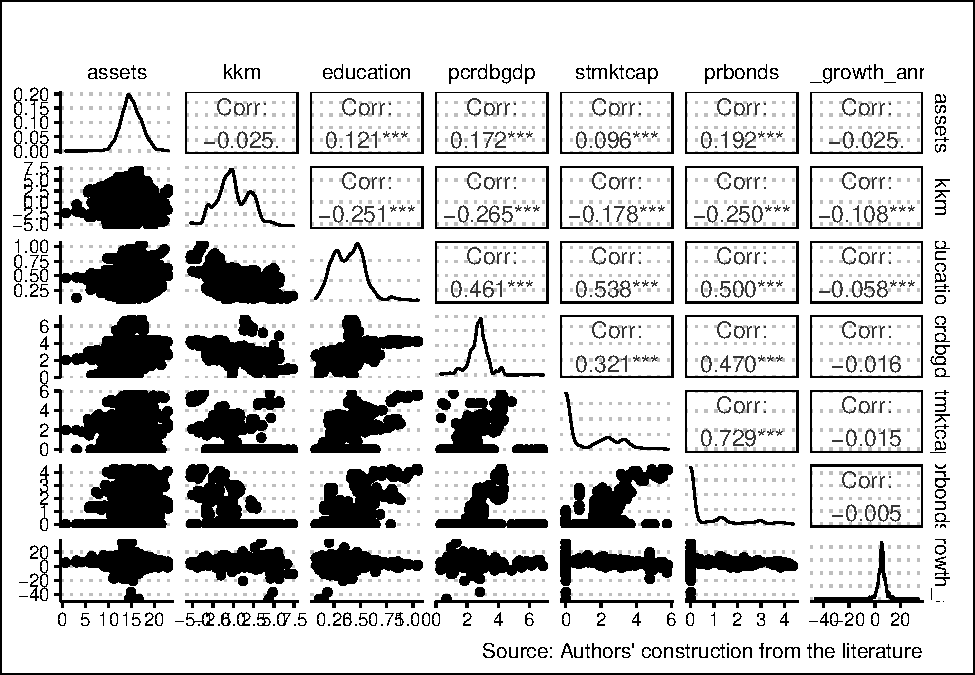
\includegraphics{_main_files/figure-latex/unnamed-chunk-25-1.pdf}
\caption{\label{fig:unnamed-chunk-25}Correlations Between Independent Variables}
\end{figure}

\begin{figure}
\centering
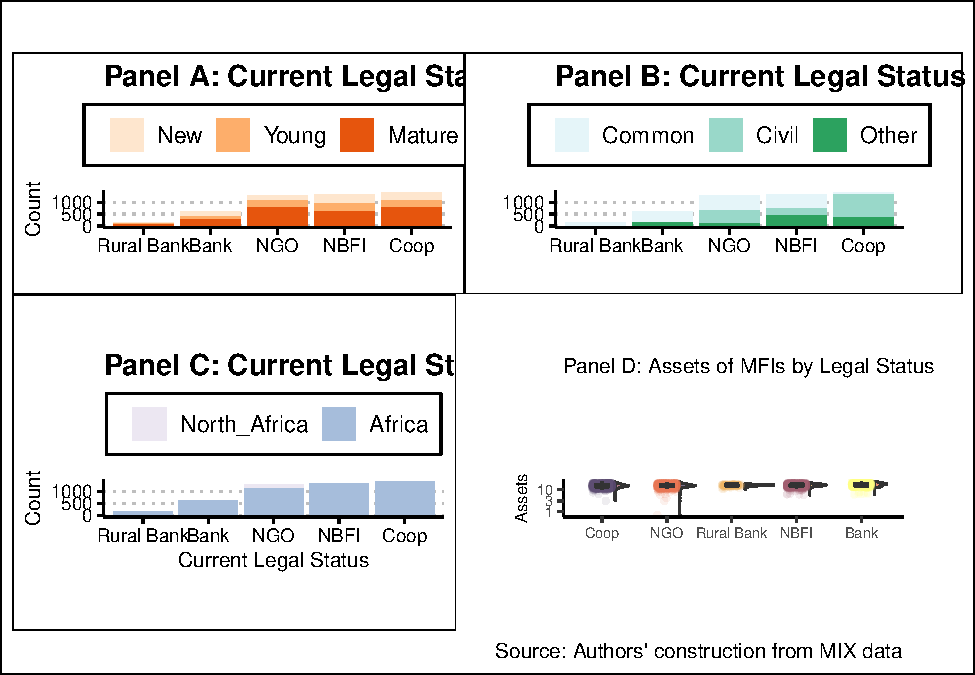
\includegraphics{_main_files/figure-latex/unnamed-chunk-30-1.pdf}
\caption{\label{fig:unnamed-chunk-30}Distribution and Asset Base of MFIs in Africa by Legal Status}
\end{figure}

\begin{figure}
\centering
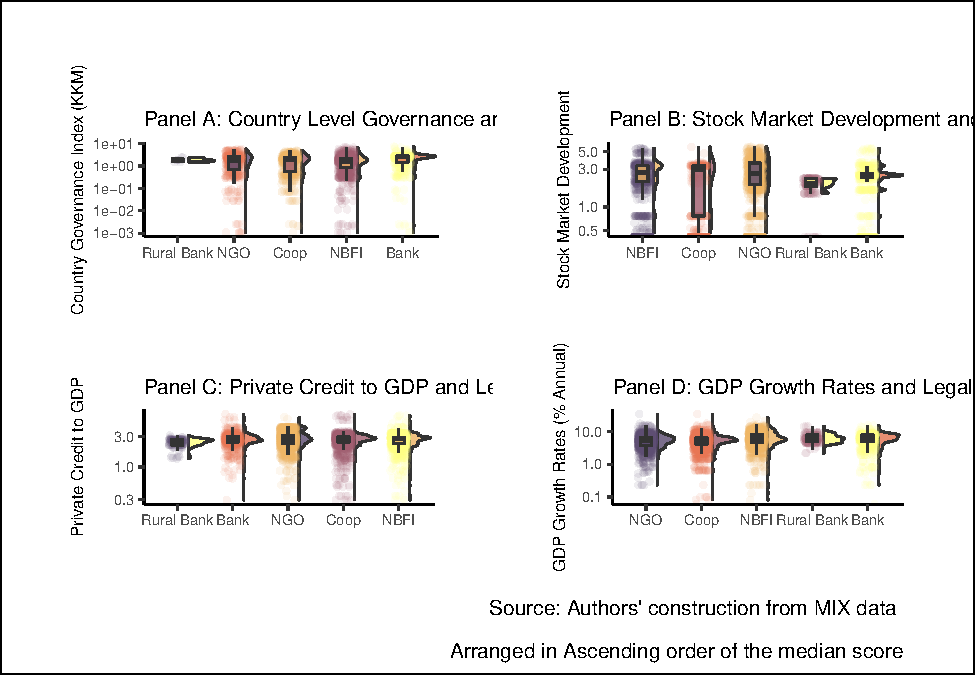
\includegraphics{_main_files/figure-latex/unnamed-chunk-31-1.pdf}
\caption{\label{fig:unnamed-chunk-31}Governance, Capital Market Development and Legal Status of MFIs in Africa}
\end{figure}

\end{landscape}

\newpage

\hypertarget{summary-statistics}{%
\subsubsection{Summary Statistics}\label{summary-statistics}}

Categorical variables summarised in Table 2 have no missing values. There are 1,280 NGOs against 3502 MFIs that are either commercial banks (619), NBFIs (1318), cooperatives (1427), and rural banks (138). As noted, even with the transformation of MFIs, NGOs still form a substantial number of MFIs, with the country to country variations \autocite{d2017ngos}. While 2558 MFIs are mature, 1200 are new, and 1024 are young. The result may indicate a slowdown in the establishment of new MFIs as donations become more unreliable. 1877 MFIs are from common law countries, with Civil law countries accounting for 1849, while 1056 come from other legal traditions. It is notable, as shown in Appendix 6, that most countries in Africa are either common law (18) or civil law(19), with very few nations in the `other' legal traditions category (11) \autocite{oto2014distribution}. It is also worth noting that North Africa accounts for only 166 observations in the data against 4616 observations in the sample dataset. Table 3 shows the summary statistics for the numeric variables where assets, governance (KKM), and GDP growth rates account for the highest variation.

Table 4 and Table 7 shows that NGOs, NBFIs, and commercial banks dominate common law countries. In civil law countries, it is cooperatives, NGOs, and NFIs that are most prevalent. In other legal traditions, it is NBFIs and credit unions that dominate. The result could indicate that the relatively well-developed capital markets in common law countries allow private, for-profit MFIs to thrive while not displacing NGOs. It means that NGOs in common law countries mostly serve niche markets where commercial MFIs find it uneconomical to reach. Weak capital markets in civil law countries mean that cooperatives are central, with NGOs playing a significant role. Commercial MFIs like commercial banks and cooperatives presence is low due to capital constraints. Turning to age in Table 5, most of the mature MFIs in the sample data are cooperatives, NGOs, and commercial banks in that order, while most of the new MFIs are NBFIs, cooperatives and commercial banks, respectively. The results could indicate the increasing acceptance of the commercial model with newer MFIs going commercial. Table 6 shows the correlation between age and size, with larger MFIs more likely to be older.

\begin{table}

\caption{\label{tab:unnamed-chunk-32}Summary statistics for categorical variables}
\centering
\begin{tabular}[t]{ll}
\toprule
Variable & Counts\\
\midrule
currentlegaldummy & oth: 3502, NGO: 1280\\
currentlegalstatus & Coo: 1427, NBF: 1318, NGO: 1280, Ban: 619\\
age & Mat: 2558, New: 1200, You: 1024\\
legal\_tradition & Com: 1877, Civ: 1849, Oth: 1056\\
region & Afr: 4616, Nor: 166\\
\bottomrule
\multicolumn{2}{l}{\rule{0pt}{1em}\textit{Source: }}\\
\multicolumn{2}{l}{\rule{0pt}{1em}Authors' construction from MIX data}\\
\end{tabular}
\end{table}

\begin{table}

\caption{\label{tab:unnamed-chunk-33}Summary statistics for numeric variables}
\centering
\begin{tabular}[t]{lrrrrrrrr}
\toprule
Variable & Complete & Mean & SD & Min & Q1 & Median & Q3 & Max\\
\midrule
assets & 1 & 14.946 & 2.262 & 0.693 & 13.540 & 14.858 & 16.416 & 22.98\\
kkm & 1 & 0.003 & 2.006 & -5.233 & -1.304 & -0.114 & 1.628 & 7.37\\
education & 1 & 0.387 & 0.144 & 0.075 & 0.273 & 0.386 & 0.487 & 1.05\\
pcrdbgdp & 1 & 2.719 & 0.685 & 0.298 & 2.386 & 2.758 & 3.052 & 6.88\\
stmktcap & 1 & 1.141 & 1.473 & 0.000 & 0.000 & 0.000 & 2.428 & 5.80\\
\addlinespace
prbonds & 1 & 0.632 & 1.093 & 0.000 & 0.000 & 0.000 & 1.130 & 4.36\\
gdp\_growth\_annual & 1 & 5.310 & 3.590 & -46.082 & 4.000 & 5.420 & 6.723 & 33.63\\
\bottomrule
\multicolumn{9}{l}{\rule{0pt}{1em}\textit{Source: }}\\
\multicolumn{9}{l}{\rule{0pt}{1em}Authors' construction from MIX data}\\
\end{tabular}
\end{table}

\begin{table}

\caption{\label{tab:unnamed-chunk-34}Legal Status of MFIs in Africa by Disaggregated by Legal Tradition}
\centering
\begin{tabular}[t]{lrrrrr}
\toprule
  & NGO & Bank & NBFI & Coop & Rural Bank\\
\midrule
Common & 0.323 & 0.246 & 0.310 & 0.048 & 0.073\\
Civil & 0.304 & 0.014 & 0.158 & 0.524 & 0.001\\
Other & 0.106 & 0.126 & 0.420 & 0.348 & 0.000\\
\bottomrule
\multicolumn{6}{l}{\rule{0pt}{1em}\textit{Source: }}\\
\multicolumn{6}{l}{\rule{0pt}{1em}Authors' construction from MIX data}\\
\multicolumn{6}{l}{\rule{0pt}{1em}\textit{Note: }}\\
\multicolumn{6}{l}{\rule{0pt}{1em}\textsuperscript{1} Horizontals total to 100}\\
\end{tabular}
\end{table}

\newpage

\hypertarget{results-of-the-regression-model}{%
\subsection{Results of the Regression Model}\label{results-of-the-regression-model}}

Table 11 shows the output from both the logit and probit regression analysis. We ran the analysis using the full dataset, then filter MFIs with three or more years and five or more years of data and rerun the regression. While most of the variables are significant, it is notable that there is also a robust time trend towards commercialisation of MFIs, indicating relatively fewer NGO type MFIs over time. The trend is indicative of the gains that the sustainability school has made. However, NGOs still form a substantial proportion of MFIs. In this section, we examine each variable and its relative contribution to the transformation of MFIs. Note that we use the logit model in column 1 of Table 9 to interpret the discussion results. However, the interpretation is also valid for the other models presented in the Table.

\hypertarget{age}{%
\subsubsection{Age}\label{age}}

New MFIs are more likely to adopt a commercial model than either young or mature ones, given the coefficients' negative sign. The observation may reflect the increasing acceptance of the financial systems approach to microfinance, making it harder for new entrants to attract donor funding \autocite{d2017ngos}. We postulate that older MFIs, being the pioneers and hence already are well-acquainted with donors, find it easier to continue raising funds through donations and elicit state subsidies \autocite{d2013unsubsidized,mia2017mission}. Established MFIs have a historical relationship with donors. They are likely to attract funds, more so from donors that favour the welfare approach to microfinance of reaching out to the financially excluded first before pursuing profits. The results are in line with those in Table 5, which shows the distribution of MFI legal status disaggregated by age. While only 18\% of NGOs are new, over 30\% are mature, an upward trend. By comparison, the other legal status either decline or are relatively constant.

\begin{table}

\caption{\label{tab:unnamed-chunk-35}Legal Status of MFIs in Africa by Disaggregated by Age}
\centering
\begin{tabular}[t]{lrrrrr}
\toprule
  & NGO & Bank & NBFI & Coop & Rural Bank\\
\midrule
New & 0.188 & 0.193 & 0.297 & 0.295 & 0.027\\
Young & 0.273 & 0.099 & 0.334 & 0.275 & 0.019\\
Mature & 0.303 & 0.112 & 0.242 & 0.309 & 0.034\\
\bottomrule
\multicolumn{6}{l}{\rule{0pt}{1em}\textit{Source: }}\\
\multicolumn{6}{l}{\rule{0pt}{1em}Authors' construction from MIX data}\\
\end{tabular}
\end{table}

Examining the coefficients, when an MFI rises from being new to young, it is 0.474 as likely to be in the commercial category than the new MFIs, ceteris paribus. This result means that new MFIs are likely to be commercial while older MFIs are most likely NGOs. \footnote{Relative risk ratios allow for easier interpretation of the logit models. To compute the ratio, we exponentiate the coefficients. For instance, the coefficient for young MFIs is -0.747, so the relative risk ratio is \(e^{-0.747}\) which gives 0.474. In other words, the odds of having commercial model of microfinance is 1 - 0.474 = 0.526 in the sample dataset.}, we find that keeping all the other variables constant, young MFIs roughly one half less likely to be commercial than new MFIs. Likewise, mature MFIs are a third as likely to be commercial compared to new MFIs. The finding is also consistent with the intense time effect towards commercialisation which points to the increased acceptance of the commercial model of MFIs.

Having started their operations before the neo-liberal tradition took hold, older MFIs have created goodwill with donors that enable them to solicit donations and subsidies easily. Mature MFIs could also have evolved business models that allow them to be financially sustainable without converting to the commercial model. For instance, mature MFIs tend to have a broader asset base meaning they have a more diverse customer base (see Table 6). Besides, they may have embedded the emphasis on the social mission in their vision, mission, and organisational cultures to such an extent that both the MFI and the donor community find it hard to pull back \autocite{ramus2017,berbegal2019impact}.

\begin{table}

\caption{\label{tab:unnamed-chunk-36}Size (Assets) of MFIs in Africa by Disaggregated by Age}
\centering
\begin{tabular}[t]{lrrrr}
\toprule
Age & Min\_size & Mean\_size & Median\_size & Max\_size\\
\midrule
New & 0.693 & 13.5 & 13.5 & 23.0\\
Young & 5.796 & 14.5 & 14.4 & 19.8\\
Mature & 6.361 & 15.8 & 15.7 & 22.9\\
\bottomrule
\multicolumn{5}{l}{\rule{0pt}{1em}\textit{Source: }}\\
\multicolumn{5}{l}{\rule{0pt}{1em}Authors' construction from MIX data}\\
\end{tabular}
\end{table}

Younger MFIs, on the other hand, cropped up when the paradigm shift to the institutional approach was taking shape. It means, therefore, that donors were reluctant to extend funds to such organisations. Hence, the MFIs had to supplement the little donor funding and government subsidies by raising funds from the capital markets. The thinking is consistent with the literature that shows the extent to which donor funding is volatile and especially sensitive to geopolitical realignments \autocite{garmaise2013cheap,d2017aid} and business cycles \autocite{wagner2013vulnerability}.

\hypertarget{legal-tradition}{%
\subsubsection{Legal Tradition}\label{legal-tradition}}

As noted, we have grouped countries in the sample data into their respective legal traditions following \textcite{oto2014distribution}. MFIs in civil law countries have a higher chance of transformation compared to those from common law countries \footnote{Appendix 6 shows a breakdown of the legal traditions in Africa}. However, MFIs located in countries under ``other'' legal traditions have the highest likelihood of adopting the commercial model. The result is in line with the literature that shows the law's central place in finance \autocite{la2013law}. Specifically, holding all other variables constant, MFIs in civil law countries are 0.656 (\(e^{-0.421}\)) as likely as those in common law countries to follow the commercial model, meaning that most of them remain NGOs, following the not-for-profit, welfare approach. The odds of MFIs in civil law countries being commercial is 0.344 (\(1 - 0.656\)). On the contrary, MFIs in countries that follow other legal traditions are twice (\(e^{0.744}\)) as likely to be commercial instead of NGOs, with the odds being 1.1 (\(2.1 - 1.1\)).

\begin{table}

\caption{\label{tab:unnamed-chunk-37}Breakdown of Legal Status of MFIs by Legal Traditions, Percent}
\centering
\begin{tabular}[t]{lrrrrr}
\toprule
legal\_tradition & NGO & Bank & NBFI & Coop & Rural Bank\\
\midrule
Common & 47.34 & 74.47 & 44.2 & 6.38 & 99.275\\
Civil & 43.91 & 4.04 & 22.2 & 67.91 & 0.725\\
Other & 8.75 & 21.49 & 33.7 & 25.72 & -\\
\bottomrule
\multicolumn{6}{l}{\rule{0pt}{1em}\textit{Source: }}\\
\multicolumn{6}{l}{\rule{0pt}{1em}Authors' construction from MIX data}\\
\multicolumn{6}{l}{\rule{0pt}{1em}\textit{Note: }}\\
\multicolumn{6}{l}{\rule{0pt}{1em}\textsuperscript{1} Verticals total to 100}\\
\end{tabular}
\end{table}

Table 4 show the breakdown of MFI legal forms by the country's legal tradition. The tables show the dominance of NGOs (32.3\%), commercial banks (24.6\%) and NBFIs (31\%) in common law countries. Cooperatives (52.4\%), NGOs (30.4\%), and NBFIs (15.8\%) dominate civil law countries, while NBFIs (42\%), cooperatives (34.8\%), and banks (12.6\%) are more common in other legal traditions. There are very few banks (1.4\%) and NBFIs (15.8\%) in civil law countries. Given the low levels of financial development in many civil law countries, there is a commercially viable gap for commercial MFIs to fill. The gap raises the odds of MFI transformation happening more frequently in civil law countries.

On the contrary, the prevalence of commercial MFIs in common law countries could hold due to the higher levels of capital market development, reflecting the relative ease of acquiring funds \autocite{schnyder2018twenty}. The relative ease of acquiring capital from stock and bond markets could make it less likely that NGOs would prevail, making the commercial model more appropriate. The substantial number of NGOs in common law countries would fill the gap left by commercial MFIs due to the infeasibility of serving the clients, for instance, due to geographic remoteness or extreme poverty. There is little literature in law and finance that examines other legal traditions, such as Portuguese/ Spanish traditions as in Mozambique, Angola, Equatorial Guinea, and countries with unique traditions like Ethiopia that was never a colony. The results for the ``other'' legal practices in Africa's setting warrant further analysis. Table 7 confirms these results, showing, for instance, that 47.34\% of NGOs are in common law countries, 43.91 in civil law countries and the rest in other legal traditions. Common law countries have the bulk of banks (74.47\%) and NBFIs (44.2\%). Rural banks are almost entirely a common law phenomenon.

\hypertarget{size-log-of-total-assets}{%
\subsubsection{Size (Log of Total Assets)}\label{size-log-of-total-assets}}

All else being constant, larger MFIs in terms of assets are more likely to adopt the commercial model than the relatively smaller MFIs with fewer assets. Perhaps large MFIs can sustain their operations independent of donations and subsidies \autocite{d2013unsubsidized}. They have a higher capacity to attract money from the capital markets, given their strong assets base and track record. Everything else remaining the same, a unit increase in the asset base of an MFI raises the probability of transformation by 1.27 (\(e^{0.240}\)), with the odds of being in the commercial model being 0.27 (\(1.27 - 1\)).

Abundant literature in Africa and beyond, such as \textcite{gwatidzo2009corporate} and \textcite{kodongo2015capital}, show that the size of an MFI is an essential determinant of firms' capital structures, the mix of long term sources of funds. In this case, larger firms could easily avail collateral for funds and tend to be more open in providing information that financial intermediaries require to assess creditworthiness. On the other hand, small firms are information opaque \autocite{beck2014sme,kersten2017small}. Small firms, for example, may not afford to generate audited financial reports. Moreover, larger firms are likely to be mature with a solid business record which creates goodwill among the providers of funds \autocite{beck2008finance}. The size of MFIs could also reflect the extent of property rights protection that is harder to enforce in countries with weak governance \autocite{johnson2002property,claessens2003financial}. A fragile institutional environment makes it difficult for firms to grow due, in part, to poor access to capital and the high costs of formalising business \autocite{hansen2004reconsidering}. Next, we examine country-level governance / institutional quality.

\hypertarget{country-level-governance-institutional-quality-kkm}{%
\subsubsection{Country Level Governance/ Institutional Quality (KKM)}\label{country-level-governance-institutional-quality-kkm}}

We capture governance or institutional quality by taking the first principal component of the KKM Worldwide Governance Indicators (WGI) indices \autocite{kraay2010worldwide}. Governance (KKM Index) positively relates to the odds of transforming. All else remaining the same, when the governance index in a country rises by one unit, MFIs in the given country are 1.1 (\(e^{0.095}\)) times more likely to be in the commercial model than NGOs, meaning that the odds rise by \(0.1\) (\(1.1 - 1\)). The results probably hold due to the importance of property rights in raising confidence among private investors who finance the operations of transformed MFIs (Allen et al., 2013, 2014). Where governance, and hence property rights are weak, then most MFIs would likely remain NGOs for longer as investors are reluctant to finance private ventures in line with \textcite{johnson2002property} and \textcite{claessens2003financial}.

Literature shows a positive link between country-level institutional quality and the establishment, growth of private firms \autocite{sobel2008testing}. As captured in the KKM index, institutional quality captures factors that relate directly to the ease of doing business, contract enforcement effectiveness, and the extent of property rights. Where institutional quality is high, we expect private firms to take root, mainly commercial MFIs, primarily commercial banks and NBFIs. On the other hand, where institutional quality is low, NGOs and not-for-profit oriented MFIs may be more prevalent \autocite{kuzey2021link}. Indeed, The results on governance could partly explain the prevalence of NGOs in North Africa in the sample dataset, together with religion. Table 8 shows that North Africa fares poorly compared to Sub-Saharan Africa in most governance metrics. In contrast, Table 9 shows that commercial banks and NBFIs are more prevalent in countries with higher institutional quality.

\begin{table}

\caption{\label{tab:unnamed-chunk-38}Summary Statistics on Governance in Africa}
\centering
\begin{tabular}[t]{lrrrr}
\toprule
Region & Min & Mean & Median & Max\\
\midrule
North Africa & -3.01 & -1.61 & -1.506 & -1.01\\
Sub-Saharan Africa & -5.23 & 0.06 & -0.114 & 7.37\\
\bottomrule
\multicolumn{5}{l}{\rule{0pt}{1em}\textit{Source: }}\\
\multicolumn{5}{l}{\rule{0pt}{1em}Authors' construction from MIX data}\\
\end{tabular}
\end{table}

\begin{table}

\caption{\label{tab:unnamed-chunk-39}Institutional Quality (KKM) and Legal Status of MFIs in Africa}
\centering
\begin{tabular}[t]{lrrrr}
\toprule
currentlegalstatus & Min & Mean & Median & Max\\
\midrule
NGO & -5.23 & -0.494 & -0.758 & 5.68\\
Bank & -5.23 & 0.929 & 1.208 & 7.37\\
NBFI & -5.17 & 0.510 & 0.350 & 6.74\\
Coop & -3.36 & -0.166 & -0.270 & 4.92\\
Rural Bank & -3.31 & -2.652 & -3.183 & 2.38\\
\bottomrule
\multicolumn{5}{l}{\rule{0pt}{1em}\textit{Source: }}\\
\multicolumn{5}{l}{\rule{0pt}{1em}Authors' construction from MIX data}\\
\end{tabular}
\end{table}

\hypertarget{private-credit-to-gdp}{%
\subsubsection{Private Credit to GDP}\label{private-credit-to-gdp}}

The private credit to GDP inversely relates to the prevalence of commercial models of microfinance, with the relationship mostly insignificant. In this case, private credit refers to an aspect of capital markets development, mainly in the banking sector. It is puzzling that a well-developed credit market does not appear to enhance the prevalence of for-profit MFI models. The results could suggest a weak linkage between MFIs and capital markets, more so credit from financial intermediaries. Indeed, MFIs exist to serve markets where mainstream intermediaries neglect, meaning the low presence of mainstream banks means a higher prevalence of MFIs to fill the void \autocite{de2007economics}. Where significant, a unit increase in private credit to GDP corresponds to a 0.894 times lower chance that an MFI will be commercial, profit-oriented (\(e^{-0.112}\)), which corresponds to an odds of -0.114.

As noted, MFIs, especially the NGO type, exist to fill a financing gap that results from the failure of credit markets to reach the financially excluded - the poor, rural dwellers and women savers and borrowers. If mainstream credit markets are functional, then there is no case for the existence of commercial MFIs, because mainstream banks would fill the gap adequately, leaving no business case for commercial MFIs to exist. However, as no credit market is fully efficient, then NGOs would exist to serve niche markets where financial sustainability is unattainable due to a combination of high costs and low revenues \autocite{de2007economics}. On the other hand, if capital markets are not well developed, there exists a market gap that commercial MFIs could exploit to make a profit \autocite{d2013unsubsidized,armendariz2013subsidy}.

\hypertarget{stock-market-capitalisation-to-gdp}{%
\subsubsection{Stock market capitalisation to GDP}\label{stock-market-capitalisation-to-gdp}}

Stock market capitalisation to GDP has a significant negative relationship with the prevalence of commercial MFIs. Precisely, a unit increase of stock market capitalisation corresponds to a 0.721 odds of an MFI adopting the for-profit model. Like private credit to GDP, stock market capitalisation to GDP proxies the level of stock market development, an essential source of long time finance for corporations, presumably including MFIs. The equity could be from the public or private equity market, which the stock market would proxy reasonably well. In the case of MFIs in the sample dataset, the capital assets ratio- the ratio of equity capital to assets shows the importance of equity in financing microfinance. Notably, equity is of greater importance to NGOs than commercial MFIs (see Table 10 below), with NBFIs and commercial banks following in that order. If NGOs are the dominant participants in equity markets, then there are lower chances that a well-developed stock market corresponds to more commercial MFIs. The same argument follows that if stock markets are well developed, then private and public credit markets are also well-developed \autocite{schnyder2018twenty}. With well-developed capital markets, financial exclusion incidences are fewer, leaving no vacuum that commercial MFIs could profitably exploit. In such instances, NGOs following the not-for-profit welfare model best serve the few financial exclusion instances.

\begin{table}

\caption{\label{tab:unnamed-chunk-40}Capital Asset Ratio by MFI Legal Status in Africa}
\centering
\begin{tabular}[t]{lrr}
\toprule
Legal Status & Mean & Median\\
\midrule
Bank & 0.306 & 0.239\\
Credit Union/ Cooperative & 0.196 & 0.208\\
NBFI & 0.388 & 0.324\\
NGO & 0.418 & 0.381\\
Rural Bank & 0.176 & 0.137\\
\bottomrule
\multicolumn{3}{l}{\rule{0pt}{1em}\textit{Source: }}\\
\multicolumn{3}{l}{\rule{0pt}{1em}Authors' construction from MIX data}\\
\end{tabular}
\end{table}

\hypertarget{gdp-annual-growth-rate}{%
\subsubsection{GDP Annual Growth Rate}\label{gdp-annual-growth-rate}}

The GDP growth rate is not a significant driver of transformation. Where significant, some of the coefficients are positive, while others are negative. The implication is that the macro-environment may not be a substantial driver of MFIs decisions. Most MFIs in developing countries serve the informal sector's financially excluded population with low linkage to the formal economy \autocite{ghosh2013microfinance}.

\hypertarget{regional-divide}{%
\subsubsection{Regional Divide}\label{regional-divide}}

It is notable that for the sample data, all the MFIs operating in North Africa are NGOs, while the rest of Africa has a MIX of all forms of MFIs \footnote{Countries in North Africa in the sample data are Morocco and Tunisia}. Religion may be at play in this case, where interest-based for-profit lending is incompatible with the Muslim faith that dominates North Africa \autocite{hassan2018religious}. Also, as noted, North Africa fares worse in governance (KKM) than sub-Saharan Africa, leading to a flawed property rights regime that discourages private investment \autocite{johnson2002property,claessens2003financial}.

\hypertarget{time-effects}{%
\subsubsection{Time Effects}\label{time-effects}}

There is a strong trend towards commercialisation, with the commercial model increasingly dominating Africa's MFI landscape. All the year dummies are significant in all the models, the lowest level of significance being 10\%. Numerous researchers have noted the trend towards the commercial model. Hence, the abundant research seeks to examine the potential effects of the transformation on financial inclusion targets- the financially excluded \autocite{d2017ngos}. Some scholars claim that the trend may harm financial inclusion. \autocite{meagher2006microfinance,hartarska2007regulated}. Others hold the opposing view \autocite{duvendack2015mis}. It appears that the financial sustainability school that seeks commercialisation has the upper hand in Africa, at least in the last two decades.

\newpage

\begin{landscape}

\begin{table}[!htbp] \centering 
  \caption{Regression Results - Logit and Probit Models [Coefficients]} 
  \label{} 
\footnotesize 
\begin{tabular}{@{\extracolsep{5pt}}lcccccccc} 
\\[-1.8ex]\hline 
\hline \\[-1.8ex] 
 & \multicolumn{8}{c}{\textit{Dependent variable:}} \\ 
\cline{2-9} 
\\[-1.8ex] & \multicolumn{8}{c}{dummy} \\ 
\\[-1.8ex] & \textit{logistic} & \textit{probit} & \textit{logistic} & \textit{probit} & \textit{logistic} & \textit{probit} & \textit{logistic} & \textit{probit} \\ 
\\[-1.8ex] & (1) & (2) & (3) & (4) & (5) & (6) & (7) & (8)\\ 
\hline \\[-1.8ex] 
 ageYoung & $-$0.747$^{***}$ & $-$0.421$^{***}$ & $-$0.418$^{***}$ & $-$0.240$^{***}$ & $-$0.452$^{***}$ & $-$0.264$^{***}$ & $-$0.766$^{***}$ & $-$0.431$^{***}$ \\ 
  & (0.114) & (0.065) & (0.132) & (0.076) & (0.157) & (0.091) & (0.112) & (0.064) \\ 
  & & & & & & & & \\ 
 ageMature & $-$1.200$^{***}$ & $-$0.691$^{***}$ & $-$0.898$^{***}$ & $-$0.522$^{***}$ & $-$0.944$^{***}$ & $-$0.551$^{***}$ & $-$1.150$^{***}$ & $-$0.662$^{***}$ \\ 
  & (0.106) & (0.060) & (0.122) & (0.071) & (0.145) & (0.084) & (0.104) & (0.059) \\ 
  & & & & & & & & \\ 
 legal\_traditionCivil & $-$0.421$^{***}$ & $-$0.239$^{***}$ & $-$0.515$^{***}$ & $-$0.313$^{***}$ & $-$0.545$^{***}$ & $-$0.338$^{***}$ & $-$0.518$^{***}$ & $-$0.289$^{***}$ \\ 
  & (0.117) & (0.068) & (0.127) & (0.074) & (0.140) & (0.082) & (0.114) & (0.066) \\ 
  & & & & & & & & \\ 
 legal\_traditionOther & 0.744$^{***}$ & 0.387$^{***}$ & 0.790$^{***}$ & 0.416$^{***}$ & 0.870$^{***}$ & 0.466$^{***}$ & 0.743$^{***}$ & 0.387$^{***}$ \\ 
  & (0.132) & (0.073) & (0.149) & (0.084) & (0.167) & (0.094) & (0.130) & (0.072) \\ 
  & & & & & & & & \\ 
 assets & 0.240$^{***}$ & 0.142$^{***}$ & 0.355$^{***}$ & 0.214$^{***}$ & 0.450$^{***}$ & 0.270$^{***}$ & 0.242$^{***}$ & 0.144$^{***}$ \\ 
  & (0.019) & (0.011) & (0.024) & (0.014) & (0.029) & (0.016) & (0.018) & (0.011) \\ 
  & & & & & & & & \\ 
 kkm & 0.095$^{***}$ & 0.057$^{***}$ & 0.102$^{***}$ & 0.063$^{***}$ & 0.139$^{***}$ & 0.087$^{***}$ & 0.115$^{***}$ & 0.067$^{***}$ \\ 
  & (0.019) & (0.011) & (0.023) & (0.013) & (0.025) & (0.015) & (0.019) & (0.011) \\ 
  & & & & & & & & \\ 
 pcrdbgdp & $-$0.112 & $-$0.049 & $-$0.127 & $-$0.047 & $-$0.221$^{**}$ & $-$0.097$^{*}$ & 0.055 & 0.036 \\ 
  & (0.076) & (0.042) & (0.083) & (0.047) & (0.090) & (0.051) & (0.070) & (0.039) \\ 
  & & & & & & & & \\ 
 stmktcap & $-$0.327$^{***}$ & $-$0.190$^{***}$ & $-$0.369$^{***}$ & $-$0.225$^{***}$ & $-$0.398$^{***}$ & $-$0.246$^{***}$ & $-$0.359$^{***}$ & $-$0.206$^{***}$ \\ 
  & (0.038) & (0.022) & (0.042) & (0.024) & (0.047) & (0.027) & (0.037) & (0.021) \\ 
  & & & & & & & & \\ 
 gdp\_growth\_annual & 0.016 & 0.012$^{*}$ & $-$0.004 & $-$0.0004 & $-$0.025$^{*}$ & $-$0.013 & 0.024$^{**}$ & 0.015$^{**}$ \\ 
  & (0.011) & (0.006) & (0.013) & (0.008) & (0.014) & (0.008) & (0.011) & (0.006) \\ 
  & & & & & & & & \\ 
 Constant & $-$2.030$^{***}$ & $-$1.260$^{***}$ & $-$3.600$^{***}$ & $-$2.240$^{***}$ & $-$4.510$^{***}$ & $-$2.770$^{***}$ & $-$1.480$^{***}$ & $-$0.929$^{***}$ \\ 
  & (0.446) & (0.266) & (0.507) & (0.301) & (0.569) & (0.336) & (0.277) & (0.162) \\ 
  & & & & & & & & \\ 
\hline \\[-1.8ex] 
Year Effects & Yes & Yes & Yes & Yes & Yes & Yes & No & No \\ 
Deviance & 677*** & 664*** & 651*** & 648*** & 660*** & 659*** & 619*** & 607*** \\ 
df & 29 & 29 & 29 & 29 & 29 & 29 & 9 & 9 \\ 
Data & Full & Full & >3yrs & >3yrs & >5yrs & >5yrs & Full & Full \\ 
Observations & 4,782 & 4,782 & 3,840 & 3,840 & 3,165 & 3,165 & 4,782 & 4,782 \\ 
Log Likelihood & $-$2,439.000 & $-$2,446.000 & $-$2,004.000 & $-$2,005.000 & $-$1,633.000 & $-$1,633.000 & $-$2,469.000 & $-$2,475.000 \\ 
Akaike Inf. Crit. & 4,939.000 & 4,952.000 & 4,068.000 & 4,071.000 & 3,325.000 & 3,326.000 & 4,957.000 & 4,969.000 \\ 
\hline 
\hline \\[-1.8ex] 
\textit{Note:}  & \multicolumn{8}{r}{$^{*}$p$<$0.1; $^{**}$p$<$0.05; $^{***}$p$<$0.01} \\ 
\end{tabular} 
\end{table}

\end{landscape}

\newpage

\hypertarget{multinomial-logit-model}{%
\subsection{Multinomial Logit Model}\label{multinomial-logit-model}}

We extend the analysis to the multinomial logit model. The results are presented in the tables in Appendix 2 to Appendix 5. As in the binary models, the results confirm the factors that drive the conversion of MFIs from NGOs to commercial models. We examine for each variable the interpretation from the model basing our discussion on the results in Appendix 2, which easily generalises to the other Tables in the series. The results show that as the MFI transitions from being new to young, it is less likely to be a bank, NBFI, credit union, or rural bank due to the coefficients' negative sign. Hence, older firms are more likely NGOs in line with the logit model for reasons expounded in the logit model's output.

Similarly, compared to NGOs, mature MFIs are less likely to be commercial banks, NBFIs, cooperatives or rural banks. The results are in line with the logit model showing that most commercial MFIs are more likely new or young, while NGOs are more likely mature. Again, start-up MFIs are more inclined to the commercial model than the established firms.

Relative to common law countries, MFIs in civil law countries less likely to be commercial banks, NBFIs, and rural banks and are more likely to be NGOs. However, in civil law countries, MFIs are more likely to be cooperatives than NGOs. Likewise, relative to common law countries, MFIs in other legal traditions are less likely to be commercial banks and rural banks and more likely to be credit unions or NBFIs. The results illustrate the link between legal tradition and the legal status of MFIs, with NGOs dominating common law countries whilst cooperatives prevail in other legal traditions, including civil law tradition. As noted, the better-developed capital markets in common law countries leave little room for commercial MFIs to thrive. On the contrary, the under-served populace in civil law countries presents ample business opportunities for profit-oriented MFIs \autocite{d2013unsubsidized,mia2017mission}.

The results show that as an MFI size increases, the likelihood of shifting from the NGO model to the commercial model rises. However, as firms grow in size, they are less likely to adopt the cooperative model, although the relationship is not significant. MFIs mainly shift from NGOs to commercial banks and NBFIs, but rarely to cooperatives or rural banks. The results highlight the uniqueness of cooperatives and rural banking as microfinance models that serve niche markets. Strictly speaking, cooperatives are quasi-commercial entities. Their mode of operation differs from the other MFIs in terms of clientele and possible geographic reach, hence reducing size. Similarly, rural banks serve marginalised rural dwellers and are more prevalent in common law countries. Noting that most large MFIs are also mature, it follows that the edge granted by maturity also accrues to larger MFIs \autocite{beck2014sme,kersten2017small}.

Also, as country-level institutional quality rises, MFIs are more likely to be commercial banks and NBFIs, and less likely cooperatives and rural banks relative to NGOs. Cooperatives and rural banks are less sensitive to institutional quality matters courtesy of their unique markets, even more so than NGOs \autocite{sobel2008testing}. As noted, the commercial, for-profit model could only thrive best in countries where institutional quality is high. However, cooperatives and rural bank in Africa serve unique markets, with rural banks primarily focused on informal rural economies that may have a weak linkage to the formal economy, making governance and institutional quality less relevant.

Capital market development- both stock market to GDP and private credit to GDP follow a similar pattern. As in the logit model, MFIs located in countries scoring high in private credit to GDP and stock market capitalisation to GDP are less likely to go commercial and more likely to be NGOs. We have argued before that well developed financial market implies a smaller customer base for MFIs and hence the result. The result also concurs with the observation of legal tradition. Because capital markets in civil law countries are less developed, the void tends to be profitably filled by commercial MFIs.In common law countries, capital markets leave few profitable opportunities which NGOs serve \autocite{d2013unsubsidized,armendariz2013subsidy}.

Finally, high GDP growth rates increase the likelihood that an MFI will be a commercial bank, NBFI, or rural bank but less likely to be a cooperative or rural bank. As is the case with institutional quality, the economic environment matters most for commercial MFIs that target profit. However, NGOs, cooperatives and rural bank may better serve communities undergoing adverse economic experiences \autocite{ghosh2013microfinance}. Cooperatives obtain capital from members and are obligated to attend to the members regardless of the economic uncertainties. NGOs and rural banks specifically target marginalised people. Economic downturns are more likely to raise the level of exclusion and make these forms of MFIs even more relevant \autocite{schnyder2018twenty}.

\newpage

\hypertarget{overall-model-fit}{%
\subsection{Overall Model Fit}\label{overall-model-fit}}

To assess the overall model fit, we generate the \texttt{confusion\ matrix}. For this purpose, we use the models developed by using the whole dataset- Table 11 for the logit model and Appendix 2 for the multinomial logit model.

\hypertarget{logit-model}{%
\subsubsection{Logit Model}\label{logit-model}}

Overall, the models are highly significant (at 1\% significance levels, see Table 11), meaning that they explain why MFIs tend to adopt to given model better than guessing the most prevalent outcome- every MFI in the sample is not an NGO. In the first row of Table 12, we see that the logit model predicted correctly that 304 NGOs were NGOs. The model also accurately predicts that an MFI belongs to other legal forms (Bank, NBFI, Coop, Rural Bank) when they belong to these forms. However, the model fails by predicting 976 cases of MFIs as other legal forms when they are NGOs. Similarly, the model wrongly classifies 126 cases of MFIs of other legal forms as NGOs.

Overall, the logit model accurately predicts the legal status of an MFI 77\% of the time \footnote{The accuracy is computed as (304 + 3376) / (304 + 976 + 126 + 3376) = 0.77}. The prediction is within the confidence interval captured by the entries \texttt{AccuracyLower} and \texttt{AccuracyUpper}. If we were to guess that every MFI in the dataset follows the commercial model (that is, not an NGO), we would be accurate 73.2\% of the time (referred to as the No Information Rate (NIR) in the \texttt{confusion\ matrix}) \autocite{cavalin2018confusion}. The p-value shows that the accuracy is not due to chance with over 99\% confidence, meaning that the accuracy is significantly greater than the NIR \autocite{kleinbaum2002logistic}.

The model has low \texttt{sensitivity}, though, at 23.75\%. In this case, sensitivity is a model's ability to accurately predict that an MFI is an NGO when it is an NGO \autocite{marom2010using}. The low \texttt{sensitivity} could, in part, be due to the low \texttt{prevalence} of NGOs in the dataset (at 26.77\%) relative to the commercial forms of MFIs (73.23\%). However, the model has very high \texttt{specificity} at 96.4\%. Specificity is the capacity of the model to predict that an MFI follows the commercial model (NOT an NGO) when it following the commercial model (is NOT an NGO) \autocite{zeng2020confusion}. Hence, it appears that commercial MFIs have distinct characters that easily allow the model to distinguish them from NGOs. The other metric of interest is the \texttt{balanced\ accuracy} that averages \texttt{sensitivity} and \texttt{specificity} at 60\% \autocite{gorzalczany2016multi}. Overall, the model does better than guessing that every MFI in the sample dataset follows the commercial model (or is NOT an NGO) \autocite{hosmer2013applied}.

\begin{table}

\caption{\label{tab:unnamed-chunk-44}Confusion Matrix and Statistics for the Logit Model}
\centering
\begin{tabular}[t]{ll}
\toprule
Description & Value\\
\midrule
Pred\_NGO\_Ref\_NGO & 304.000\\
Pred\_others\_Ref\_NGO & 976.000\\
Pred\_NGO\_Ref\_others & 126.000\\
Pred\_others\_Ref\_others & 3376.000\\
Accuracy & 0.770\\
\addlinespace
Kappa & 0.255\\
AccuracyLower & 0.757\\
AccuracyUpper & 0.781\\
NoInformationRate & 0.732\\
AccuracyPValue & 0.000\\
\addlinespace
McnemarPValue & 0.000\\
Sensitivity & 0.237\\
Specificity & 0.964\\
Pos.Pred.Value & 0.707\\
Neg.Pred.Value & 0.776\\
\addlinespace
Precision & 0.707\\
Recall & 0.237\\
F1 & 0.356\\
Prevalence & 0.268\\
Detection.Rate & 0.064\\
\addlinespace
Detection.Prevalence & 0.090\\
Balanced.Accuracy & 0.601\\
\bottomrule
\multicolumn{2}{l}{\rule{0pt}{1em}\textit{Source: }}\\
\multicolumn{2}{l}{\rule{0pt}{1em}Authors' construction}\\
\multicolumn{2}{l}{\rule{0pt}{1em}\textit{Notes: }}\\
\multicolumn{2}{l}{\rule{0pt}{1em}\textsuperscript{1} Accuracy > NoInformationRate is significant at 1\% confidence level, p = 0.0000}\\
\end{tabular}
\end{table}

\hypertarget{multinomial-logit-model-1}{%
\subsubsection{Multinomial Logit Model}\label{multinomial-logit-model-1}}

As noted, I develop the \texttt{confusion\ matrix} using the \texttt{multinomial\ logit} with the full data (Table 13). The matrix shows that the overall \texttt{accuracy} is 56.5\%. Note that the overall accuracy is one value for the entire model, the \texttt{No\ Information\ Rate\ (NIR)}. Overall \texttt{accuracy}, in this case, is the ability to accurately predict that an MFI is an NGO when it is an NGO, a commercial bank when it is a commercial bank, and so on. If we were to guess that every MFI in the model is the cooperative - the most prevalent legal form- we would be right 39.3\% of the time, the NIR. The p-value shows that the overall \texttt{accuracy} metric is significantly different from the \texttt{NIR}. Although the multinomial logit model has a markedly lower accuracy than the logit model, it has a far more demanding task of distinguishing 5 legal forms of MFIs instead of 2 for the logit model \autocite{kwak2002multinomial}.

The model's \texttt{sensitivity} varies from a low of 47.1\% for NBFI to a high of 61.8\% for NGOs. The \texttt{specificity} is relatively high, ranging from 80.1\% for NBFIs to 99.22\% for rural banks \autocite{ginting2019hate}. NGOs have a \texttt{specificity} of 81.4\%, meaning that the model can predict that an MFI is not an NGO when it is not an NGO 81.4\% of the time. For rural banks, the model can correctly predict over 99\% of the time that an MFI is not a rural bank when it is not a rural bank. The \texttt{balanced\ accuracy} is also reasonably high, with the lowest being NBFIs at 63.9\% and the highest at 79.26\% for rural banks \autocite{hedeker2003mixed}.

\newpage

\begin{table}

\caption{\label{tab:unnamed-chunk-45}Confusion Matrix and Statistics for the Multinomial Logit Model}
\centering
\begin{tabular}[t]{lrrrrr}
\toprule
  & NGO & Bank & NBFI & Coop & Rural Bank\\
\midrule
Accuracy & 0.565 & 0.565 & 0.565 & 0.565 & 0.565\\
NoInformationRate & 0.393 & 0.393 & 0.393 & 0.393 & 0.393\\
Kappa & 0.414 & 0.414 & 0.414 & 0.414 & 0.414\\
sensitivity & 0.618 & 0.615 & 0.478 & 0.584 & 0.593\\
specificity & 0.814 & 0.930 & 0.801 & 0.886 & 0.992\\
\addlinespace
PosPredValue & 0.437 & 0.517 & 0.474 & 0.768 & 0.739\\
NegPredValue & 0.901 & 0.952 & 0.803 & 0.767 & 0.985\\
Prevalence & 0.189 & 0.109 & 0.274 & 0.393 & 0.036\\
DetectionRate & 0.117 & 0.067 & 0.131 & 0.229 & 0.021\\
DetectionPrevalence & 0.268 & 0.129 & 0.276 & 0.298 & 0.029\\
\addlinespace
BalancedAccuracy & 0.716 & 0.773 & 0.639 & 0.735 & 0.793\\
\bottomrule
\multicolumn{6}{l}{\rule{0pt}{1em}\textit{Source: }}\\
\multicolumn{6}{l}{\rule{0pt}{1em}Authors' construction}\\
\multicolumn{6}{l}{\rule{0pt}{1em}\textit{Notes: }}\\
\multicolumn{6}{l}{\rule{0pt}{1em}\textsuperscript{1} Accuracy > NoInformationRate is significant at 1\% confidence level, p = 0.0000}\\
\end{tabular}
\end{table}

\newpage

\hypertarget{regression-diagnostics}{%
\subsection{Regression Diagnostics}\label{regression-diagnostics}}

This section examines three issues that arise in logit models; extreme values, multicollinearity, and linearity, respectively.

\hypertarget{extreme-values}{%
\subsubsection{Extreme values}\label{extreme-values}}

Figure 4 below shows that the data indeed has influential values. For robustness, we winsorise the data, removing the top 10\% and the bottom 10\%. Still, the results remain robust, as regression results in Table 14 shows. It is notable that apart from the change in coefficients' value, the signs remain the same, meaning that influential observations are not a significant issue.

\begin{table}[!htbp] \centering 
  \caption{Regression Results - Logit and Probit Models for Winsorized Data} 
  \label{} 
\footnotesize 
\begin{tabular}{@{\extracolsep{5pt}}lcccc} 
\\[-1.8ex]\hline 
\hline \\[-1.8ex] 
 & \multicolumn{4}{c}{\textit{Dependent variable:}} \\ 
\cline{2-5} 
\\[-1.8ex] & \multicolumn{4}{c}{dummy} \\ 
\\[-1.8ex] & \textit{logistic} & \textit{probit} & \textit{logistic} & \textit{probit} \\ 
\\[-1.8ex] & (1) & (2) & (3) & (4)\\ 
\hline \\[-1.8ex] 
 ageYoung & $-$0.885$^{***}$ & $-$0.514$^{***}$ & $-$0.888$^{***}$ & $-$0.515$^{***}$ \\ 
  & (0.119) & (0.068) & (0.117) & (0.067) \\ 
  & & & & \\ 
 ageMature & $-$1.320$^{***}$ & $-$0.772$^{***}$ & $-$1.250$^{***}$ & $-$0.728$^{***}$ \\ 
  & (0.112) & (0.063) & (0.109) & (0.062) \\ 
  & & & & \\ 
 legal\_traditionCivil & $-$0.215$^{*}$ & $-$0.110 & $-$0.369$^{***}$ & $-$0.192$^{***}$ \\ 
  & (0.130) & (0.076) & (0.124) & (0.072) \\ 
  & & & & \\ 
 legal\_traditionOther & 0.916$^{***}$ & 0.502$^{***}$ & 0.894$^{***}$ & 0.486$^{***}$ \\ 
  & (0.145) & (0.080) & (0.142) & (0.079) \\ 
  & & & & \\ 
 assets & 0.269$^{***}$ & 0.159$^{***}$ & 0.270$^{***}$ & 0.162$^{***}$ \\ 
  & (0.021) & (0.012) & (0.020) & (0.012) \\ 
  & & & & \\ 
 kkm & 0.084$^{***}$ & 0.052$^{***}$ & 0.115$^{***}$ & 0.069$^{***}$ \\ 
  & (0.021) & (0.012) & (0.021) & (0.012) \\ 
  & & & & \\ 
 pcrdbgdp & $-$0.335$^{***}$ & $-$0.190$^{***}$ & $-$0.083 & $-$0.052 \\ 
  & (0.098) & (0.056) & (0.086) & (0.050) \\ 
  & & & & \\ 
 stmktcap & $-$0.269$^{***}$ & $-$0.153$^{***}$ & $-$0.328$^{***}$ & $-$0.184$^{***}$ \\ 
  & (0.044) & (0.025) & (0.041) & (0.024) \\ 
  & & & & \\ 
 gdp\_growth\_annual & 0.028 & 0.019$^{*}$ & 0.040$^{**}$ & 0.025$^{**}$ \\ 
  & (0.018) & (0.010) & (0.017) & (0.010) \\ 
  & & & & \\ 
 Constant & $-$2.100$^{***}$ & $-$1.290$^{***}$ & $-$1.660$^{***}$ & $-$1.030$^{***}$ \\ 
  & (0.485) & (0.289) & (0.326) & (0.191) \\ 
  & & & & \\ 
\hline \\[-1.8ex] 
Year Effects & Yes & Yes & No & No \\ 
Deviance & 664*** & 657*** & 602*** & 595*** \\ 
df & 29 & 29 & 9 & 9 \\ 
Data & Winsorized & Winsorized & Winsorized & Winsorized \\ 
Observations & 4,450 & 4,450 & 4,450 & 4,450 \\ 
Log Likelihood & $-$2,269.000 & $-$2,273.000 & $-$2,300.000 & $-$2,304.000 \\ 
Akaike Inf. Crit. & 4,598.000 & 4,605.000 & 4,620.000 & 4,627.000 \\ 
\hline 
\hline \\[-1.8ex] 
\textit{Note:}  & \multicolumn{4}{r}{$^{*}$p$<$0.1; $^{**}$p$<$0.05; $^{***}$p$<$0.01} \\ 
\end{tabular} 
\end{table}

\begin{landscape}

\begin{figure}
\centering
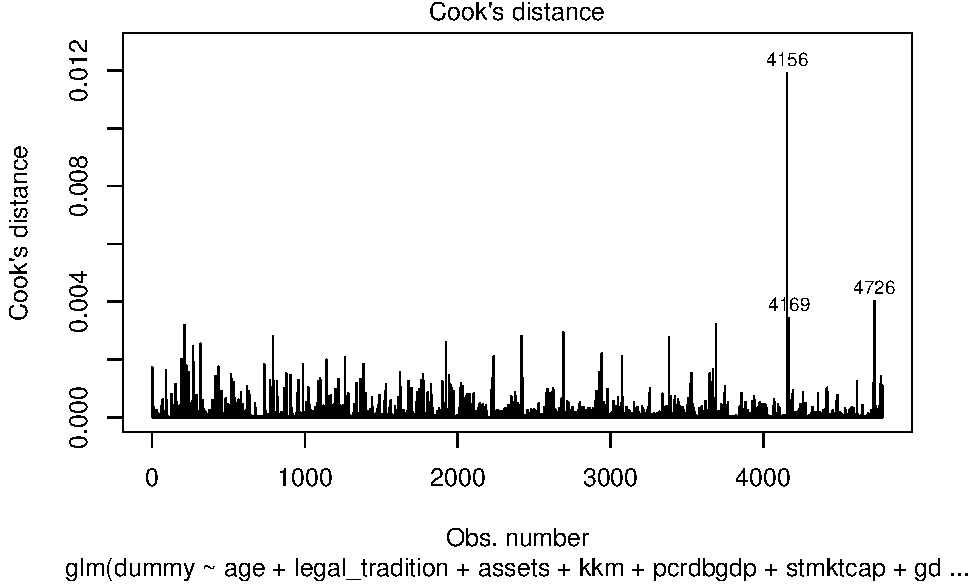
\includegraphics{_main_files/figure-latex/unnamed-chunk-49-1.pdf}
\caption{\label{fig:unnamed-chunk-49}Visualisation of Outliers}
\end{figure}

\end{landscape}

\hypertarget{multicollinearity}{%
\subsubsection{Multicollinearity}\label{multicollinearity}}

The problem of multicollinearity among independent variables leads to unstable coefficients. In the model, however, multicollinearity is not a significant issue as in all cases, the variance inflation factors(VIFs) are below the 5 (sometimes 10) threshold that several researchers recommend \autocite{gujarati2012econometrics}. Table 15 shows the VIFs for each variable.

\begin{table}

\caption{\label{tab:unnamed-chunk-50}Variance Inflation Factors for Logit Model}
\centering
\begin{tabu} to \linewidth {>{\raggedright}X>{\raggedleft}X>{\raggedleft}X>{\raggedleft}X}
\toprule
  & GVIF & Df & GVIF\textasciicircum{}(1/(2*Df))\\
\midrule
age & 1.41 & 2 & 1.09\\
legal\_tradition & 2.57 & 2 & 1.27\\
assets & 1.49 & 1 & 1.22\\
kkm & 1.16 & 1 & 1.08\\
pcrdbgdp & 2.01 & 1 & 1.42\\
\addlinespace
stmktcap & 2.72 & 1 & 1.65\\
gdp\_growth\_annual & 1.15 & 1 & 1.07\\
factor(year) & 1.59 & 20 & 1.01\\
\bottomrule
\multicolumn{4}{l}{\rule{0pt}{1em}\textit{Source: }}\\
\multicolumn{4}{l}{\rule{0pt}{1em}Authors' construction}\\
\end{tabu}
\end{table}

\hypertarget{linearity-assumptions}{%
\subsubsection{Linearity assumptions}\label{linearity-assumptions}}

Here, we check the linear relationship between independent numeric variables and the logit of the outcome by visually inspecting the scatter plot between each predictor and the logit values. As Figure 5 below shows, most of the variables could reasonably fit a linear model, though not perfectly \autocite{cheng2007testing}. The fitted line uses the Locally Weighted Scatterplot Smoothing (LOESS) method hence the perceived non-linearity.

\begin{landscape}

\begin{figure}
\centering
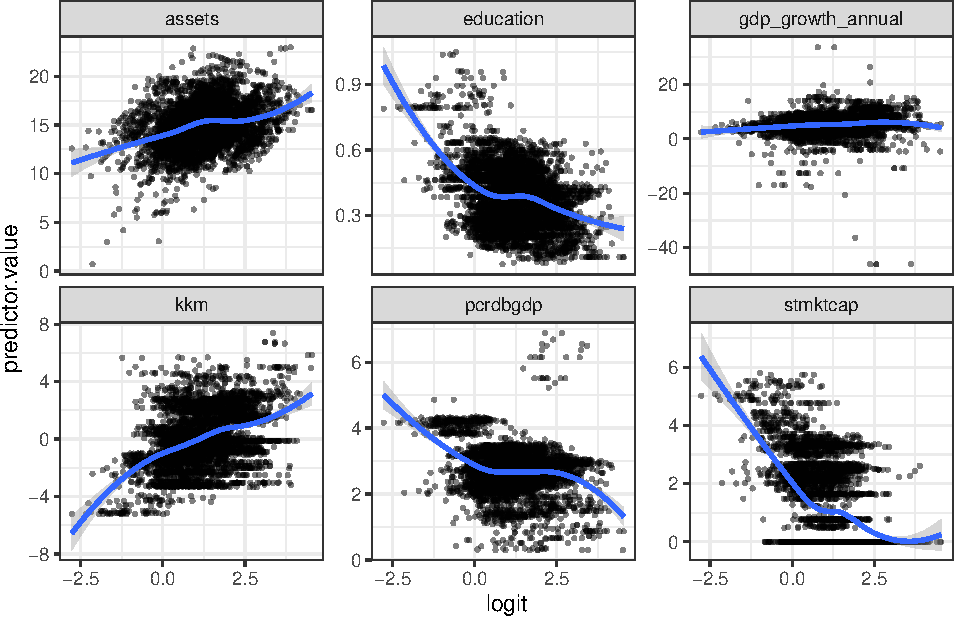
\includegraphics{_main_files/figure-latex/unnamed-chunk-51-1.pdf}
\caption{\label{fig:unnamed-chunk-51}Linearity of Independent Variables}
\end{figure}

\end{landscape}

\hypertarget{other-robustness-checks}{%
\subsection{Other Robustness Checks}\label{other-robustness-checks}}

In many cases, it is unlikely that a credit union starts as an NGO, given that they mostly serve clients with similar professional base and geographic background. For this reason, we run a regression, excluding cooperatives with the results displayed in Appendix 1. The results remain robust in this case, noting that signs of the coefficients do not change.

\hypertarget{conclusion}{%
\section{Conclusion}\label{conclusion}}

This article examined the factors that drive the transformation of MFIs from the NGO not-for-profit model to the commercial, for-profit model focusing on Africa. The analysis shows that at the MFI level, there are two critical factors; age, legal tradition, and size matter. At the aggregate level, it is the country institutional quality and stock market capitalisation that matter. Specifically, older firms are most likely to follow the not-for-profit model, while newer firms are most likely commercial. We expect that older firms are better at attracting donations and subsidies and hence still follow the earlier tradition of microfinance as a welfare tool to aid the financially excluded \autocite{d2017ngos}. For legal tradition, MFIs located in civil law countries are least likely to follow the commercial model relative to those in common law countries. The results align with the finance and law literature, where civil law countries have weaker capital markets. Hence, MFIs have a market void to fill profitably, unlike in common law countries where mainstream markets already fill much of the gap leaving relatively fewer profit opportunities \autocite{la2013law,schnyder2018twenty}.MFIs in countries following other legal traditions other than common law and civil law are most likely to follow the commercial model.

Turning to size, larger firms tend to adopt the commercial model compared to relatively younger firms. We expect that larger firms are better at attracting commercial capital courtesy of the goodwill and the collateral to pledge. Institutional quality relates positively to adopting the commercial model at the country level, while stock market capitalisation has the opposite effect. Institutional quality has this effect due to the ease of contracting, contract enforcement, and property rights \autocite{claessens2003financial}. Private credit to GDP and GDP growth rates are not significant drivers of the conversion of MFIs. However, the coefficients' signs indicate that private credit to GDP, like the stock market to GDP ratio, is inversely related to the probability of transformation. At the same time, GDP growth shows mixed effects.

\hypertarget{appendices}{%
\section{Appendices}\label{appendices}}

\hypertarget{appendix-1-logit-and-probit-models-excluding-cooperatives}{%
\subsection{Appendix 1: Logit and Probit Models Excluding Cooperatives}\label{appendix-1-logit-and-probit-models-excluding-cooperatives}}

\begin{table}[!htbp] \centering 
  \caption{Regression Results - Logit and Probit Models with Data Excluding Cooperatives} 
  \label{} 
\footnotesize 
\begin{tabular}{@{\extracolsep{5pt}}lcc} 
\\[-1.8ex]\hline 
\hline \\[-1.8ex] 
 & \multicolumn{2}{c}{\textit{Dependent variable:}} \\ 
\cline{2-3} 
\\[-1.8ex] & \multicolumn{2}{c}{dummy} \\ 
\\[-1.8ex] & \textit{logistic} & \textit{probit} \\ 
\\[-1.8ex] & (1) & (2)\\ 
\hline \\[-1.8ex] 
 ageYoung & $-$0.747$^{***}$ & $-$0.421$^{***}$ \\ 
  & (0.114) & (0.065) \\ 
  & & \\ 
 ageMature & $-$1.200$^{***}$ & $-$0.691$^{***}$ \\ 
  & (0.106) & (0.060) \\ 
  & & \\ 
 legal\_traditionCivil & $-$0.421$^{***}$ & $-$0.239$^{***}$ \\ 
  & (0.117) & (0.068) \\ 
  & & \\ 
 legal\_traditionOther & 0.744$^{***}$ & 0.387$^{***}$ \\ 
  & (0.132) & (0.073) \\ 
  & & \\ 
 assets & 0.240$^{***}$ & 0.142$^{***}$ \\ 
  & (0.019) & (0.011) \\ 
  & & \\ 
 kkm & 0.095$^{***}$ & 0.057$^{***}$ \\ 
  & (0.019) & (0.011) \\ 
  & & \\ 
 pcrdbgdp & $-$0.112 & $-$0.049 \\ 
  & (0.076) & (0.042) \\ 
  & & \\ 
 stmktcap & $-$0.327$^{***}$ & $-$0.190$^{***}$ \\ 
  & (0.038) & (0.022) \\ 
  & & \\ 
 gdp\_growth\_annual & 0.016 & 0.012$^{*}$ \\ 
  & (0.011) & (0.006) \\ 
  & & \\ 
 Constant & $-$2.030$^{***}$ & $-$1.260$^{***}$ \\ 
  & (0.446) & (0.266) \\ 
  & & \\ 
\hline \\[-1.8ex] 
Year Effects & Yes & Yes \\ 
Deviance & 664*** & 657*** \\ 
df & 29 & 29 \\ 
Data & No Credit Unions & No Credit Unions \\ 
Observations & 4,782 & 4,782 \\ 
Log Likelihood & $-$2,439.000 & $-$2,446.000 \\ 
Akaike Inf. Crit. & 4,939.000 & 4,952.000 \\ 
\hline 
\hline \\[-1.8ex] 
\textit{Note:}  & \multicolumn{2}{r}{$^{*}$p$<$0.1; $^{**}$p$<$0.05; $^{***}$p$<$0.01} \\ 
\end{tabular} 
\end{table}

\newpage

\hypertarget{appendix-2-multinomial-logit-model-with-full-dataset}{%
\subsection{Appendix 2: Multinomial Logit Model With Full Dataset}\label{appendix-2-multinomial-logit-model-with-full-dataset}}

\begin{table}[!htbp] \centering 
  \caption{Regression Results - Multinomial Logit Model- Full Data} 
  \label{} 
\footnotesize 
\begin{tabular}{@{\extracolsep{5pt}}lcccc} 
\\[-1.8ex]\hline 
\hline \\[-1.8ex] 
 & \multicolumn{4}{c}{\textit{Dependent variable:}} \\ 
\cline{2-5} 
\\[-1.8ex] & Bank & NBFI & Coop & Rural Bank \\ 
\\[-1.8ex] & (1) & (2) & (3) & (4)\\ 
\hline \\[-1.8ex] 
 ageYoung & $-$1.640$^{***}$ & $-$0.621$^{***}$ & $-$0.543$^{***}$ & $-$0.973$^{***}$ \\ 
  & (0.184) & (0.133) & (0.139) & (0.374) \\ 
  & & & & \\ 
 ageMature & $-$2.650$^{***}$ & $-$1.460$^{***}$ & $-$0.630$^{***}$ & $-$0.840$^{***}$ \\ 
  & (0.174) & (0.128) & (0.128) & (0.294) \\ 
  & & & & \\ 
 legal\_traditionCivil & $-$3.750$^{***}$ & $-$1.190$^{***}$ & 1.890$^{***}$ & $-$5.130$^{***}$ \\ 
  & (0.266) & (0.143) & (0.167) & (1.070) \\ 
  & & & & \\ 
 legal\_traditionOther & $-$0.377$^{*}$ & 0.715$^{***}$ & 2.400$^{***}$ & $-$5.880$^{***}$ \\ 
  & (0.199) & (0.149) & (0.177) & (1.750) \\ 
  & & & & \\ 
 assets & 0.798$^{***}$ & 0.360$^{***}$ & $-$0.007 & 0.420$^{***}$ \\ 
  & (0.038) & (0.026) & (0.024) & (0.070) \\ 
  & & & & \\ 
 kkm & 0.450$^{***}$ & 0.250$^{***}$ & $-$0.066$^{**}$ & $-$1.480$^{***}$ \\ 
  & (0.034) & (0.024) & (0.026) & (0.185) \\ 
  & & & & \\ 
 pcrdbgdp & $-$0.008 & $-$0.048 & $-$0.250$^{***}$ & $-$2.640$^{***}$ \\ 
  & (0.109) & (0.085) & (0.091) & (0.624) \\ 
  & & & & \\ 
 stmktcap & $-$0.266$^{***}$ & $-$0.217$^{***}$ & $-$0.364$^{***}$ & $-$1.300$^{***}$ \\ 
  & (0.061) & (0.045) & (0.049) & (0.314) \\ 
  & & & & \\ 
 gdp\_growth\_annual & 0.043$^{**}$ & 0.054$^{***}$ & $-$0.005 & 0.019 \\ 
  & (0.018) & (0.014) & (0.013) & (0.079) \\ 
  & & & & \\ 
 Constant & $-$11.400$^{***}$ & $-$4.580$^{***}$ & $-$1.250$^{**}$ & $-$3.840 \\ 
  & (0.973) & (0.577) & (0.594) & (3.310) \\ 
  & & & & \\ 
\hline \\[-1.8ex] 
Year Effects & Yes & Yes & Yes & Yes \\ 
Data & Full & Full & Full & Full \\ 
Akaike Inf. Crit. & 10,124.000 & 10,124.000 & 10,124.000 & 10,124.000 \\ 
\hline 
\hline \\[-1.8ex] 
\textit{Note:}  & \multicolumn{4}{r}{$^{*}$p$<$0.1; $^{**}$p$<$0.05; $^{***}$p$<$0.01} \\ 
\end{tabular} 
\end{table}

\newpage

\hypertarget{appendix-3-multinomial-logit-model--full-data-excluding-credit-unions-cooperatives}{%
\subsection{Appendix 3: Multinomial Logit Model- Full Data Excluding Credit Unions/ Cooperatives}\label{appendix-3-multinomial-logit-model--full-data-excluding-credit-unions-cooperatives}}

\begin{table}[!htbp] \centering 
  \caption{Regression Results - Multinomial Logit Model- Full Data Without Cooperatives} 
  \label{} 
\footnotesize 
\begin{tabular}{@{\extracolsep{5pt}}lcccc} 
\\[-1.8ex]\hline 
\hline \\[-1.8ex] 
 & \multicolumn{4}{c}{\textit{Dependent variable:}} \\ 
\cline{2-5} 
\\[-1.8ex] & Bank & NBFI & Coop & Rural Bank \\ 
\\[-1.8ex] & (1) & (2) & (3) & (4)\\ 
\hline \\[-1.8ex] 
 ageYoung & $-$1.640$^{***}$ & $-$0.621$^{***}$ & $-$0.543$^{***}$ & $-$0.973$^{***}$ \\ 
  & (0.184) & (0.133) & (0.139) & (0.374) \\ 
  & & & & \\ 
 ageMature & $-$2.650$^{***}$ & $-$1.460$^{***}$ & $-$0.630$^{***}$ & $-$0.840$^{***}$ \\ 
  & (0.174) & (0.128) & (0.128) & (0.294) \\ 
  & & & & \\ 
 legal\_traditionCivil & $-$3.750$^{***}$ & $-$1.190$^{***}$ & 1.890$^{***}$ & $-$5.130$^{***}$ \\ 
  & (0.266) & (0.143) & (0.167) & (1.070) \\ 
  & & & & \\ 
 legal\_traditionOther & $-$0.377$^{*}$ & 0.715$^{***}$ & 2.400$^{***}$ & $-$5.880$^{***}$ \\ 
  & (0.199) & (0.149) & (0.177) & (1.750) \\ 
  & & & & \\ 
 assets & 0.798$^{***}$ & 0.360$^{***}$ & $-$0.007 & 0.420$^{***}$ \\ 
  & (0.038) & (0.026) & (0.024) & (0.070) \\ 
  & & & & \\ 
 kkm & 0.450$^{***}$ & 0.250$^{***}$ & $-$0.066$^{**}$ & $-$1.480$^{***}$ \\ 
  & (0.034) & (0.024) & (0.026) & (0.185) \\ 
  & & & & \\ 
 pcrdbgdp & $-$0.008 & $-$0.048 & $-$0.250$^{***}$ & $-$2.640$^{***}$ \\ 
  & (0.109) & (0.085) & (0.091) & (0.624) \\ 
  & & & & \\ 
 stmktcap & $-$0.266$^{***}$ & $-$0.217$^{***}$ & $-$0.364$^{***}$ & $-$1.300$^{***}$ \\ 
  & (0.061) & (0.045) & (0.049) & (0.314) \\ 
  & & & & \\ 
 gdp\_growth\_annual & 0.043$^{**}$ & 0.054$^{***}$ & $-$0.005 & 0.019 \\ 
  & (0.018) & (0.014) & (0.013) & (0.079) \\ 
  & & & & \\ 
 Constant & $-$11.400$^{***}$ & $-$4.580$^{***}$ & $-$1.250$^{**}$ & $-$3.840 \\ 
  & (0.973) & (0.577) & (0.594) & (3.310) \\ 
  & & & & \\ 
\hline \\[-1.8ex] 
Year Effects & Yes & Yes & Yes & Yes \\ 
Data & Full & Full & Full & Full \\ 
Akaike Inf. Crit. & 10,124.000 & 10,124.000 & 10,124.000 & 10,124.000 \\ 
\hline 
\hline \\[-1.8ex] 
\textit{Note:}  & \multicolumn{4}{r}{$^{*}$p$<$0.1; $^{**}$p$<$0.05; $^{***}$p$<$0.01} \\ 
\end{tabular} 
\end{table}

\newpage

\hypertarget{appendix-4-multinomial-logit-model-with-full-dataset-but-no-year-effects}{%
\subsection{Appendix 4: Multinomial Logit Model With Full Dataset But No Year Effects}\label{appendix-4-multinomial-logit-model-with-full-dataset-but-no-year-effects}}

\begin{table}[!htbp] \centering 
  \caption{Regression Results - Multinomial Logit Model- Full Data Without Year Effects} 
  \label{} 
\footnotesize 
\begin{tabular}{@{\extracolsep{5pt}}lcccc} 
\\[-1.8ex]\hline 
\hline \\[-1.8ex] 
 & \multicolumn{4}{c}{\textit{Dependent variable:}} \\ 
\cline{2-5} 
\\[-1.8ex] & Bank & NBFI & Coop & Rural Bank \\ 
\\[-1.8ex] & (1) & (2) & (3) & (4)\\ 
\hline \\[-1.8ex] 
 ageYoung & $-$1.740$^{***}$ & $-$0.619$^{***}$ & $-$0.543$^{***}$ & $-$1.120$^{***}$ \\ 
  & (0.181) & (0.132) & (0.136) & (0.359) \\ 
  & & & & \\ 
 ageMature & $-$2.620$^{***}$ & $-$1.400$^{***}$ & $-$0.539$^{***}$ & $-$0.822$^{***}$ \\ 
  & (0.170) & (0.126) & (0.125) & (0.284) \\ 
  & & & & \\ 
 legal\_traditionCivil & $-$3.830$^{***}$ & $-$1.290$^{***}$ & 1.700$^{***}$ & $-$5.380$^{***}$ \\ 
  & (0.264) & (0.140) & (0.163) & (1.110) \\ 
  & & & & \\ 
 legal\_traditionOther & $-$0.359$^{*}$ & 0.720$^{***}$ & 2.390$^{***}$ & $-$11.000$^{***}$ \\ 
  & (0.195) & (0.146) & (0.175) & (0.0004) \\ 
  & & & & \\ 
 assets & 0.787$^{***}$ & 0.373$^{***}$ & $-$0.006 & 0.346$^{***}$ \\ 
  & (0.036) & (0.025) & (0.023) & (0.061) \\ 
  & & & & \\ 
 kkm & 0.471$^{***}$ & 0.260$^{***}$ & $-$0.044$^{*}$ & $-$1.420$^{***}$ \\ 
  & (0.033) & (0.024) & (0.025) & (0.138) \\ 
  & & & & \\ 
 pcrdbgdp & 0.156 & 0.081 & 0.001 & $-$2.300$^{***}$ \\ 
  & (0.102) & (0.080) & (0.082) & (0.371) \\ 
  & & & & \\ 
 stmktcap & $-$0.269$^{***}$ & $-$0.248$^{***}$ & $-$0.431$^{***}$ & $-$1.110$^{***}$ \\ 
  & (0.060) & (0.044) & (0.047) & (0.239) \\ 
  & & & & \\ 
 gdp\_growth\_annual & 0.057$^{***}$ & 0.061$^{***}$ & $-$0.0003 & $-$0.027 \\ 
  & (0.016) & (0.013) & (0.012) & (0.039) \\ 
  & & & & \\ 
 Constant & $-$10.700$^{***}$ & $-$4.540$^{***}$ & $-$0.470 & $-$0.495 \\ 
  & (0.558) & (0.371) & (0.349) & (1.010) \\ 
  & & & & \\ 
\hline \\[-1.8ex] 
Year Effects & Yes & No & No & No \\ 
Data & No Coop & No Coop & No Coop & No Coop \\ 
Akaike Inf. Crit. & 10,187.000 & 10,187.000 & 10,187.000 & 10,187.000 \\ 
\hline 
\hline \\[-1.8ex] 
\textit{Note:}  & \multicolumn{4}{r}{$^{*}$p$<$0.1; $^{**}$p$<$0.05; $^{***}$p$<$0.01} \\ 
\end{tabular} 
\end{table}

\newpage

\hypertarget{appendix-5-multinomial-logit-model--full-data-excluding-credit-unions-cooperatives-and-year-effects}{%
\subsection{Appendix 5: Multinomial Logit Model- Full Data Excluding Credit Unions/ Cooperatives and Year Effects}\label{appendix-5-multinomial-logit-model--full-data-excluding-credit-unions-cooperatives-and-year-effects}}

\begin{table}[!htbp] \centering 
  \caption{Regression Results - Multinomial Logit Model- Full Data Excluding Cooperatives and Year Effects} 
  \label{} 
\footnotesize 
\begin{tabular}{@{\extracolsep{5pt}}lcccc} 
\\[-1.8ex]\hline 
\hline \\[-1.8ex] 
 & \multicolumn{4}{c}{\textit{Dependent variable:}} \\ 
\cline{2-5} 
\\[-1.8ex] & Bank & NBFI & Coop & Rural Bank \\ 
\\[-1.8ex] & (1) & (2) & (3) & (4)\\ 
\hline \\[-1.8ex] 
 ageYoung & $-$1.740$^{***}$ & $-$0.619$^{***}$ & $-$0.543$^{***}$ & $-$1.120$^{***}$ \\ 
  & (0.181) & (0.132) & (0.136) & (0.359) \\ 
  & & & & \\ 
 ageMature & $-$2.620$^{***}$ & $-$1.400$^{***}$ & $-$0.539$^{***}$ & $-$0.822$^{***}$ \\ 
  & (0.170) & (0.126) & (0.125) & (0.284) \\ 
  & & & & \\ 
 legal\_traditionCivil & $-$3.830$^{***}$ & $-$1.290$^{***}$ & 1.700$^{***}$ & $-$5.380$^{***}$ \\ 
  & (0.264) & (0.140) & (0.163) & (1.110) \\ 
  & & & & \\ 
 legal\_traditionOther & $-$0.359$^{*}$ & 0.720$^{***}$ & 2.390$^{***}$ & $-$11.000$^{***}$ \\ 
  & (0.195) & (0.146) & (0.175) & (0.0004) \\ 
  & & & & \\ 
 assets & 0.787$^{***}$ & 0.373$^{***}$ & $-$0.006 & 0.346$^{***}$ \\ 
  & (0.036) & (0.025) & (0.023) & (0.061) \\ 
  & & & & \\ 
 kkm & 0.471$^{***}$ & 0.260$^{***}$ & $-$0.044$^{*}$ & $-$1.420$^{***}$ \\ 
  & (0.033) & (0.024) & (0.025) & (0.138) \\ 
  & & & & \\ 
 pcrdbgdp & 0.156 & 0.081 & 0.001 & $-$2.300$^{***}$ \\ 
  & (0.102) & (0.080) & (0.082) & (0.371) \\ 
  & & & & \\ 
 stmktcap & $-$0.269$^{***}$ & $-$0.248$^{***}$ & $-$0.431$^{***}$ & $-$1.110$^{***}$ \\ 
  & (0.060) & (0.044) & (0.047) & (0.239) \\ 
  & & & & \\ 
 gdp\_growth\_annual & 0.057$^{***}$ & 0.061$^{***}$ & $-$0.0003 & $-$0.027 \\ 
  & (0.016) & (0.013) & (0.012) & (0.039) \\ 
  & & & & \\ 
 Constant & $-$10.700$^{***}$ & $-$4.540$^{***}$ & $-$0.470 & $-$0.495 \\ 
  & (0.558) & (0.371) & (0.349) & (1.010) \\ 
  & & & & \\ 
\hline \\[-1.8ex] 
Year Effects & No & No & No & No \\ 
Data & Full & Full & Full & Full \\ 
Akaike Inf. Crit. & 10,187.000 & 10,187.000 & 10,187.000 & 10,187.000 \\ 
\hline 
\hline \\[-1.8ex] 
\textit{Note:}  & \multicolumn{4}{r}{$^{*}$p$<$0.1; $^{**}$p$<$0.05; $^{***}$p$<$0.01} \\ 
\end{tabular} 
\end{table}

\newpage

\hypertarget{appendix-6-legal-traditions-in-africa}{%
\subsection{Appendix 6: Legal Traditions in Africa}\label{appendix-6-legal-traditions-in-africa}}

\begin{table}

\caption{\label{tab:unnamed-chunk-57}Legal Traditions in Africa}
\centering
\fontsize{7}{9}\selectfont
\begin{tabular}[t]{ll}
\toprule
Country & Legal\_Tradition\\
\midrule
Algeria & Civil\\
Benin & Civil\\
Burkina Faso & Civil\\
Cameroon & Civil\\
Central African Republic & Civil\\
\addlinespace
Chad & Civil\\
Comoros & Civil\\
Congo, Rep. & Civil\\
Cote d'Ivoire & Civil\\
Gabon & Civil\\
\addlinespace
Guinea & Civil\\
Madagascar & Civil\\
Mali & Civil\\
Mauritania & Civil\\
Morocco & Civil\\
\addlinespace
Niger & Civil\\
Senegal & Civil\\
Togo & Civil\\
Tunisia & Civil\\
Botswana & Common\\
\addlinespace
Eswatini & Common\\
Gambia, The & Common\\
Ghana & Common\\
Kenya & Common\\
Lesotho & Common\\
\addlinespace
Liberia & Common\\
Malawi & Common\\
Namibia & Common\\
Nigeria & Common\\
Sierra Leone & Common\\
\addlinespace
South Africa & Common\\
South Sudan & Common\\
Sudan & Common\\
Tanzania & Common\\
Uganda & Common\\
\addlinespace
Zambia & Common\\
Zimbabwe & Common\\
Angola & Others\\
Burundi & Others\\
Cape Verde & Others\\
\addlinespace
Congo, Dem. Rep. & Others\\
Egypt, Arab Republic of & Others\\
Equatorial Guinea & Others\\
Eritrea & Others\\
Ethiopia & Others\\
\addlinespace
Guinea-Bissau & Others\\
Mozambique & Others\\
Rwanda & Others\\
\bottomrule
\multicolumn{2}{l}{\rule{0pt}{1em}\textit{Source: }}\\
\multicolumn{2}{l}{\rule{0pt}{1em}Oto-Peralías and Romero-Ávila (2014)}\\
\multicolumn{2}{l}{\rule{0pt}{1em}\textit{Note: }}\\
\multicolumn{2}{l}{\rule{0pt}{1em}\textsuperscript{1} Other legal traditions include Spanish, Portuguese, Belgian, and Italian}\\
\multicolumn{2}{l}{\rule{0pt}{1em}\textsuperscript{2} Ethiopia is a peculiar case of a country in Africa that was not colonised}\\
\end{tabular}
\end{table}

\hypertarget{troubleshooting}{%
\chapter{Troubleshooting}\label{troubleshooting}}

This chapter describes common errors you may run into, and how to fix them.

\hypertarget{error-failed-to-build-the-bibliography-via-biber}{%
\section{Error: Failed to build the bibliography via biber}\label{error-failed-to-build-the-bibliography-via-biber}}

This can happen if you've had a failed build, perhaps in relation to RStudio shutting down abruptly.

Try doing this:

\begin{enumerate}
\def\labelenumi{\arabic{enumi}.}
\tightlist
\item
  type \texttt{make\ clean-knits} in the terminal tab (or run \texttt{file.remove(list.files(pattern\ =\ "*.(log\textbar{}mtc\textbar{}maf\textbar{}aux\textbar{}bbl\textbar{}blg\textbar{}xml)"))} in the R console) to clean up files generated by LaTeX during a build
\item
  restart your computer
\end{enumerate}

If this does not solve the problem, try using the \href{https://www.overleaf.com/learn/latex/Bibliography_management_with_natbib}{natbib} LaTeX package instead of \href{https://www.overleaf.com/learn/latex/Articles/Getting_started_with_BibLaTeX}{biblatex} for handling references.
To do this, go to \textbf{index.Rmd} and

\begin{enumerate}
\def\labelenumi{\arabic{enumi}.}
\tightlist
\item
  set \texttt{use-biblatex:\ false} and \texttt{use-natbib:\ true}
\item
  set \texttt{citation\_package:\ natbib} under
\end{enumerate}

\begin{Shaded}
\begin{Highlighting}[]
\FunctionTok{output}\KeywordTok{:}
\AttributeTok{  bookdown:}\FunctionTok{:pdf\_book}\KeywordTok{:}
\AttributeTok{    }\FunctionTok{citation\_package}\KeywordTok{:}\AttributeTok{ natbib}
\end{Highlighting}
\end{Shaded}

\begin{savequote}
Alles Gescheite ist schon gedacht worden.\\
Man muss nur versuchen, es noch einmal zu denken.

All intelligent thoughts have already been thought;\\
what is necessary is only to try to think them again.
\qauthor{--- Johann Wolfgang von Goethe \autocite{von_goethe_wilhelm_1829}}\end{savequote}



\hypertarget{conclusion-1}{%
\chapter*{Conclusion}\label{conclusion-1}}
\addcontentsline{toc}{chapter}{Conclusion}

If we don't want Conclusion to have a chapter number next to it, we can add the \texttt{\{-\}} attribute.

\hypertarget{more-info}{%
\section*{More info}\label{more-info}}
\addcontentsline{toc}{section}{More info}

And here's some other random info:
the first paragraph after a chapter title or section head \emph{shouldn't be} indented, because indents are to tell the reader that you're starting a new paragraph.
Since that's obvious after a chapter or section title, proper typesetting doesn't add an indent there.

This paragraph, by contrast, \emph{will} be indented as it should because it is not the first one after the `More info' heading.
All hail LaTeX. (If you're reading the HTML version, you won't see any indentation - have a look at the PDF version to understand what in the earth this section is babbling on about).

\startappendices

\hypertarget{the-first-appendix}{%
\chapter{The First Appendix}\label{the-first-appendix}}

This first appendix includes an R chunk that was hidden in the document (using \texttt{echo\ =\ FALSE}) to help with readibility:

\textbf{In 02-rmd-basics-code.Rmd}

\textbf{And here's another one from the same chapter, i.e.~Chapter \ref{code}:}

\hypertarget{the-second-appendix-for-fun}{%
\chapter{The Second Appendix, for Fun}\label{the-second-appendix-for-fun}}


%%%%% REFERENCES

% JEM: Quote for the top of references (just like a chapter quote if you're using them).  Comment to skip.
% \begin{savequote}[8cm]
% The first kind of intellectual and artistic personality belongs to the hedgehogs, the second to the foxes \dots
%   \qauthor{--- Sir Isaiah Berlin \cite{berlin_hedgehog_2013}}
% \end{savequote}

\setlength{\baselineskip}{0pt} % JEM: Single-space References

{\renewcommand*\MakeUppercase[1]{#1}%
\printbibliography[heading=bibintoc,title={\bibtitle}]}


\end{document}
